\documentclass[11pt]{book}
%\documentclass[a4paper,12pt]{article}

%---- from GEO4012
%\usepackage{times}
%\usepackage[margin=3cm]{geometry}
%\usepackage{setspace}
%\usepackage[authoryear]{natbib}
%\onehalfspacing
%\usepackage{xr}
%\renewcommand{\thesection}{\arabic{section}}
%---- end

%\usepackage{latexsym}
\usepackage[T1]{fontenc}
\usepackage[utf8]{inputenc}
%\usepackage[latin1]{inputenc}
\usepackage[english]{babel}
%\usepackage{mathptmx}
\usepackage{amsmath}
\usepackage{amssymb}
%\usepackage{textcomp}
%\usepackage{varioref}
\usepackage{float}
\usepackage{graphicx}
%\usepackage{pxfonts}
\usepackage{array}
\newcolumntype{L}[1]{>{\raggedright\let\newline\\\arraybackslash\hspace{0pt}}m{#1}}
\newcolumntype{C}[1]{>{\centering\let\newline\\\arraybackslash\hspace{0pt}}m{#1}}
\newcolumntype{R}[1]{>{\raggedleft\let\newline\\\arraybackslash\hspace{0pt}}m{#1}}


%\usepackage[python]{optional}
%\usepackage{listings}

%\setlength{\parindent}{0mm}

\renewcommand{\floatpagefraction}{.9}

\begin{document}
%opening
\title{Is there a positive feedback between Arctic stratus and diminishing sea ice?\\Master thesis}
\author{Mari Fenn Kristiansen}
\date{}

%\begin{document}
\maketitle
\frontmatter
\section*{Abstract}

This will be my abstract. \\
Write it later.... \\
No more than a page and should contain:\\
- main findings
- how it compares to others
- a conclusion?
\section*{Acknowledgements}

First of all I want to thank my main supervisor Jón Egill Kristjánsson for an interesting project and for the opportunity to come and work at NCAR for a couple of weeks. I also want to thank my other supervisor Kari Alterskjær for her "poking" and setting deadlines and pushing me for the past six months. I greatly appreciate their guidance and criticism throughout this project, and the doors that were always safe to knock on. 

Thank you so much to Anne Claire Fuillioux for helping me with setting up and getting started with WRF, and to both her and Kjell Andresen for help with technical problems during my work with this thesis. Thanks should also be given to Kjetil Schanke Aas for always taking time to answer any stupid WRF-related questions I might have had.

Thanks also to Gregory Thompson whom Jón Egill and I met with in Boulder, for meeting with us and answering all my e-mails about running the new aerosol-aware microphysics scheme in WRF.

These past two years have been very enjoyable in all their stress thanks to Marta and Helle especially, for all their positiveness.

Last, but not least, I would like to thank Henrik Andersen Sveinsson, for great technical help and moral support. @++

\tableofcontents


\mainmatter
\chapter{Introduction}
\label{chap:introduction}
Since 1979, the areal extent of Arctic sea ice in early autumn has shrunk by 80\% according to satellite data~\citep{NSIDC}. According to new satellite data sets, the decline appears to be particularly rapid after 2000~\citep{Wu2012}. The dramatic reduction in sea ice extent may have contributed strongly to the rapid warming of the Arctic, due to increases in latent and sensible heat fluxes from the ocean~\citep{Screen2010}, and due to the sea ice--albedo feedback~\citep{Curry1995a}. The rapid warming of the Arctic compared to the global mean has become known as "Arctic amplification"~\citep{Graversen2008}, but the reasons for this amplification are not fully understood.

Globally, low clouds have a net cooling effect reflecting solar radiation, due to their high albedo. Clouds also absorb and emit terrestrial longwave radiation, which has a warming effect at the surface. In the Arctic the solar radiation is less than at lower latitudes, and the warming effect of downwelling longwave radiation overpowers the cooling effect of reflecting shortwave radiation, since there is less to reflect, thus low clouds have a net warming effect in the Arctic~\citep{Shupe2004}. The Arctic cloud cover is dominated by low layered clouds (stratus)~\citep{Curry1996}, and so the climate effect of low clouds in the Arctic is important to study.

Decreasing sea ice extent could lead to an increase in the aerosol number concentrations in the area where ice has retreated. The open sea surface itself would lead to an increase in release of sea salt, primary organic matter and DMS (di-methyl-sulfide) to the lower atmosphere. The lack of sea ice would also increase the likelihood that the sea could be used for shipping, which would further increase the aerosol number concentration.

The enhancement of evaporation from the ocean with diminishing sea ice and the increase in aerosol number concentration from open water and shipping could lead to denser and longer-lived low clouds in the area of sea ice retreat (@cite someone). The  hypothesis of this thesis is that these clouds would then have a different radiative effect, and by that influence the further retreat of sea ice.

\section{Main goal}
Studies by~\citet{Eastman2010b} using visual cloud reports from the Arctic, with surface and satellite observations, and by~\citet{Kay2009} and~\citet{Palm2010} using lidar and radar observations have confirmed that the low-cloud amount over the Arctic oceans varies inversely with sea ice amount. This means that there is an increase in cloud amount when there is less sea ice. Therefore, one can envisage a positive feedback between shrinking sea ice (due to global warming), enhanced evaporation, increased effective cloud cover, enhanced downwelling longwave radiation and warming surface temperatures. In this thesis I will study if the aforementioned low-cloud amounts are also denser and more persistent, and could lead to an enhanced warming and reduced sea ice amount, also known as a positive feedback.

The effect of increase in aerosol concentrations from shipping and open water, and the effect of enhanced evaporation from open water are studied separately and combined. The main goal is to find whether more open ocean and/or larger aerosol loads will lead to changes in clouds that could enhance downwelling longwave radiation and decrease upwelling shortwave radiation, both of which have a warming effect at the surface, and therefore have a positive feedback enhancing warming of the Arctic.

%(Something citing the IPCC report 2013 on the ice conditions in the Arctic, and something about Arctic clouds and radiation?)

The findings in my thesis have been achieved by use of the Advanced Research Weather, Research and Forecasting (ARW) model, with some of the most recently developed code (by Greg Thompson~\citep{Thompson2014}) for cloud micro physics and aerosols and their effects on radiation.% The results build further on the work of other researchers @name-some-and-cite and may raise some questions for further research within the field.

\section{Area description}
The study area is in the Arctic and covers the Beaufort Sea and small parts of Alaska and Canada (figure~\ref{fig:area}).

\begin{figure}
\centering
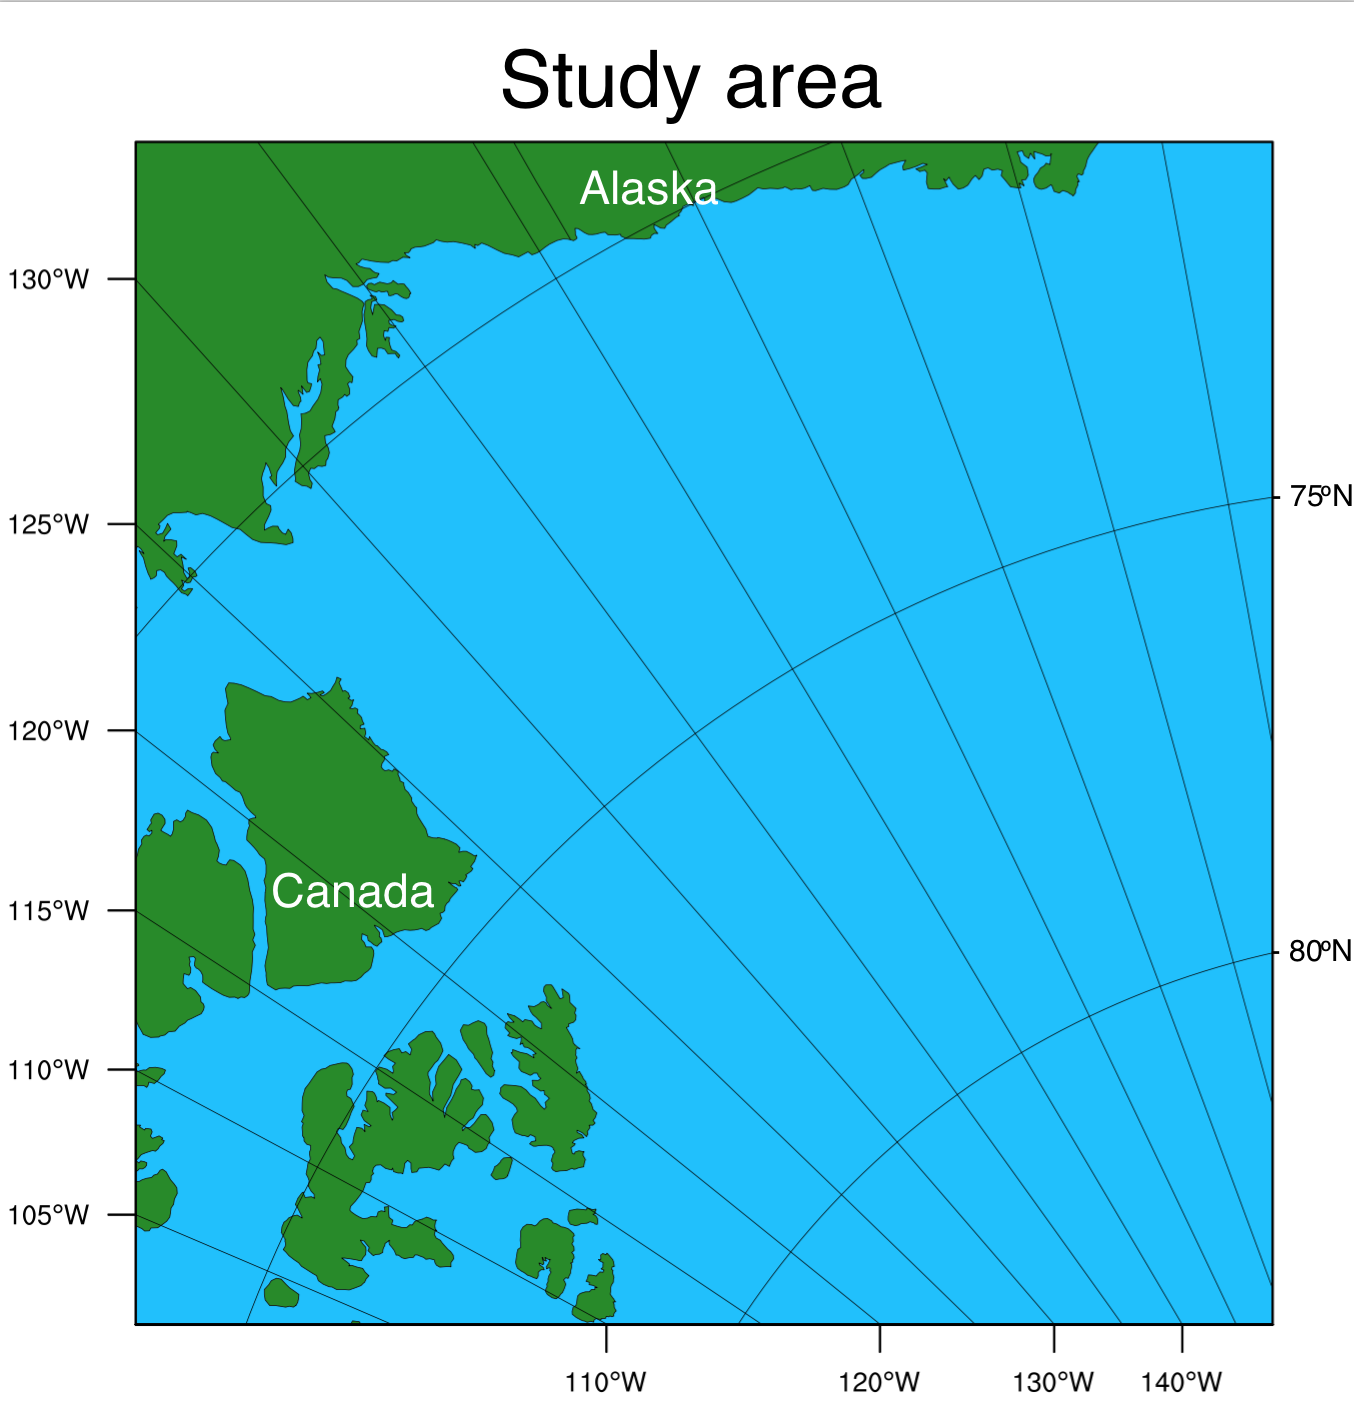
\includegraphics[width=0.7\textwidth]{introduction/studyarea.png}
\caption{An overview of the study area. The bottom right corner is the northernmost point and the y-axes show longitude and latitude to the left and right, respectively.}
\label{fig:area}
\end{figure}
 
There are a few reasons for choosing this as the study area. First it is in the Arctic, and sea ice is present there in autumn, even in 2012 when there was record low sea ice extent (eg. National Snow and Ice Data Center~\citep{NSIDC}). Also it has been subject to field campaigns: Surface Heat Budget of the Arctic Ocean (SHEBA)~\citep{Uttal2002}, First International Satellite Cloud Climatology Project Regional Experiment Arctic cloud Experiment (FIRE ACE)~\citep{Curry2000}, Mixed-Phase Arctic Cloud Experiment (M-PACE)~\citep{Verlinde2007} and more. There are a few studies on Arctic clouds that include this area and data from some of the aforementioned field campaigns. These provide parts of the science basis for my study and selection of literature and studies for comparison and questions. Quite a few studies are based on satellite data analysis, and some of these are mentioned in the next section as background and motivation for my thesis.

\section{Background}
\label{sec:background}
%Some new (and older) research that makes my thesis interesting and relevant to the field. No one has done this study with a weather forecasting model, it is interesting to look at changes in parameters in similar meteorological conditions, the same initial and boundary conditions in every run.
%Describe some of the work done by %\citet{Palm2010, Wu2012} and others on autumn low clouds in the Arctic to emphasize the importance of my work.

A study by~\citet{Schweiger2008} investigated the connection between sea ice variability and cloud cover over the Arctic seas during autumn. They analysed the ERA-40 re-analysis products and some satellite data sets. %the Television and Infrared Observation Satellite (TIROS) Operational Vertical Sounder (TOVS) Polar Pathfonder datasets~\citep{Schweiger2008}.
They found that that sea ice retreat was linked to a decrease in low-level (surface to $\sim$1.9~km) cloud amount and an increase in mid-level ($\sim$1.9 to 6.1~km) clouds. They state that the decrease in static stability and deepening of the atmospheric boundary layer, following ice retreat, contribute to the rise in cloud level. 
 %the 40-yr European Centre for Medium-Range Weather Forecasts (ECMWF) Re-Analysis (ERA-40) products

\citet{Vavrus2010} investigated the behaviour of clouds, during intervals of rapid sea ice loss in the Arctic in the 21st century. The study was done by use of the Community Climate System Model (CCSM3). They conclude that cloud changes accelerate rapid loss of sea ice in autumn. @\textit{nevne hvilke skyendringer dette er} %Their results support that cloud changes appear to accelerate rapid loss of sea ice in autumn, and possibly in winter. They also conclude that "the trends in total cloudiness during rapid ice loss events are explained almost entirely by low-level clouds" and that "a positive feedback from primarily low cloud changes amid a warming climate".

\citet{Kay2009} combined satellite data sets and complementary atmosphere reanalysis data to study the Arctic cloud and atmospheric structure during summer and early Autumn over the years 2006-2008. This covers the (at the time) record low sea ice extent from 2007. In contrast to the study by~\citet{Schweiger2008} they found more low-level cloud. The re-analysis used in~\citet{Schweiger2008} was for the time period 1964-2001, which is not the same period as~\citet{Kay2009} studied. (@\textit{finn kritikk av ERA-40, hvorfor er ikke S08 til å stole på..})

\citet{Eastman2010a} analyzed visual cloud reports from the Arctic for year-to-year variations and found that following a low-ice September there would be enhanced low cloud cover. @\textit{når? senere i sesongen? hele vinteren? sjekk!}

A study by~\citet{Palm2010} using satellite and lidar data  found that areas of open water were associated with greater polar cloud fraction. %from the Ice Cloud, and Land Elevation Satellite (ICESat) and the Cloud-Aerosol Lidar and Infrared Pathfinder Satellite Observation (CALIPSO)  found that areas of open water were associated with greater polar cloud fraction.

A common uncertainty and missing link in a few of these studies is that they did not look at liquid water content, effective radii and other parameters affecting the radiative properties of the clouds. In this study, that is what I want to look in to, how these properties are influenced by the changing sea ice, and if changes in the clouds enhance the sea ice melt.

%--------- Introduction based on master description ---------
%Since 1979, the areal extent of Arctic sea ice in early autumn has shrunk by 80\%, according to satellite data (e.g. National Snow and Ice Data Center, U.S.A.). The decline appears to be particularly rapid after 2000, as documented by new satellite data sets (Wu and Lee, 2012). The dramatic reduction in sea ice extent may have contributed strongly to the rapid warming of the Arctic observed in recent years, due to increased fluxes of sensible and latent heat from the Arctic Ocean to the overlying atmosphere (Screen and Simmonds, 2010). Other factors may also contribute such as changes in the atmospheric circulation or cloud changes. In particular, it has been suggested that the enhanced evaporation from the ice-free ocean may lead to more persistent and denser clouds. Satellite retrievals suggest that in the autumn the Arctic stratus clouds have indeed become more dense and extensive over the last 10 years, or so (Palm et al., 2010). It is well known that in the Arctic the low clouds have a warming effect on the surface due to their enhancement of downwelling radiation (Intrieri et al., 2002). Therefore, one can envisage a positive feedback between shrinking sea ice (due to global warming), enhanced evaporation, increased effective cloud cover, enhanced downwelling longwave radiation and warming surface temperatures. However, such a feedback loop has not been established, and it can not be ruled out that the positive correlation observed over only a few years between sea ice extent and cloud amount may be a co-incidence. Furthermore, cloud properties may also change due to aerosol changes, e.g., due to increasing emissions of SO2 from ship traffic, as well as di-methyl- sulfide (DMS), sea salt and primary organic matter from the open ocean. Such aerosol changes may render the clouds optically thicker (Lubin and Vogelmann, 2006), with a possible additional positive feedback loop.


%Is my work new thinking and does it seem to be very extensive?

%Should this whole chapter be a part of introduction..?

%Previous studies, shed light on why my study is interesting and may be of importance.

%Palm, Kay and Gettleman, Eastman and Warren according to the IPCC report!

\section{Structure of the thesis}
%In the following chapter~\ref{chap:background} I will present the background for my thesis; what work I hope to compare my results to and relate my thesis to. Also I will touch upon why the subject of my thesis is important. 
In the following chapter, Chapter~\ref{chap:theory}, the most important theory needed to understand some of the processes in clouds and their possible effect on the sea ice is presented. Chapter~\ref{chap:modmet} is where I explain which model and tools I have used and how I have worked with them to get the results presented and discussed in Chapter~\ref{chap:results}. A summary of main findings and conclusions are presented in the last chapter, Chapter~\ref{chap:summaryconclusions}. %introduction
\chapter{Background}
\label{chap:background}
In this chapter I shall present some recent literature on the subject. Some new (and older) research that makes my thesis interesting and relevant to the field. No one has done this study with a weather forecasting model, it is interesting to look at changes in parameters in similar meteorological conditions, the same initial and boundary conditions in every run.
Describe some of the work done by Palm2010? WuLee2012 and others on autumn low clouds in the Arctic to emphasize the importance of my work.

Is my work new thinking and does it seem to be very extensive?


\chapter{Theory}
\label{chap:theory}
\section{Arctic clouds}
The Arctic cloud cover is dominated by low clouds @cite. Most high amounts of stratus clouds are over the oceans~\citep{Klein1993}. The Arctic is the only region where the season of maximum stratus does not correspond to the season of greatest lower troposphere static stability~\citep{Klein1993}, which could be due to lack of evaporation during the cold winter months. According to~\cite{Klein1993} stratus in the Arctic basin peaks during summer at nearly 62\%, while during the winter season the stratus only accounts for 18\% of the cloud cover. This leads them to conclude that the seasonal cycle of stratus in the Arctic is driven by the temperature cycle, thereby moisture content in the atmosphere, rather than the static stability.(, as opposed to other areas.)

Are there any typical cloud properties special to the arctic? CURRY!


The air in the Arctic is very stable in winter (polar night) and clean as there are not many sources for pollution. In Autumn the sea ice extent reaches a minimum after the summer melting and leave open water to influence low clouds and their properties. 

Low clouds have bases below 2000 m. Stratus (St) are layered clouds that form when extensive areas of stable air are lifted. Stratus clouds are normally between 0.5 and 1~km thick, whereas they can be several km wide (@citeAguadoBurtpage188?).

\begin{figure}
\label{fig:dropletsize}
\centering
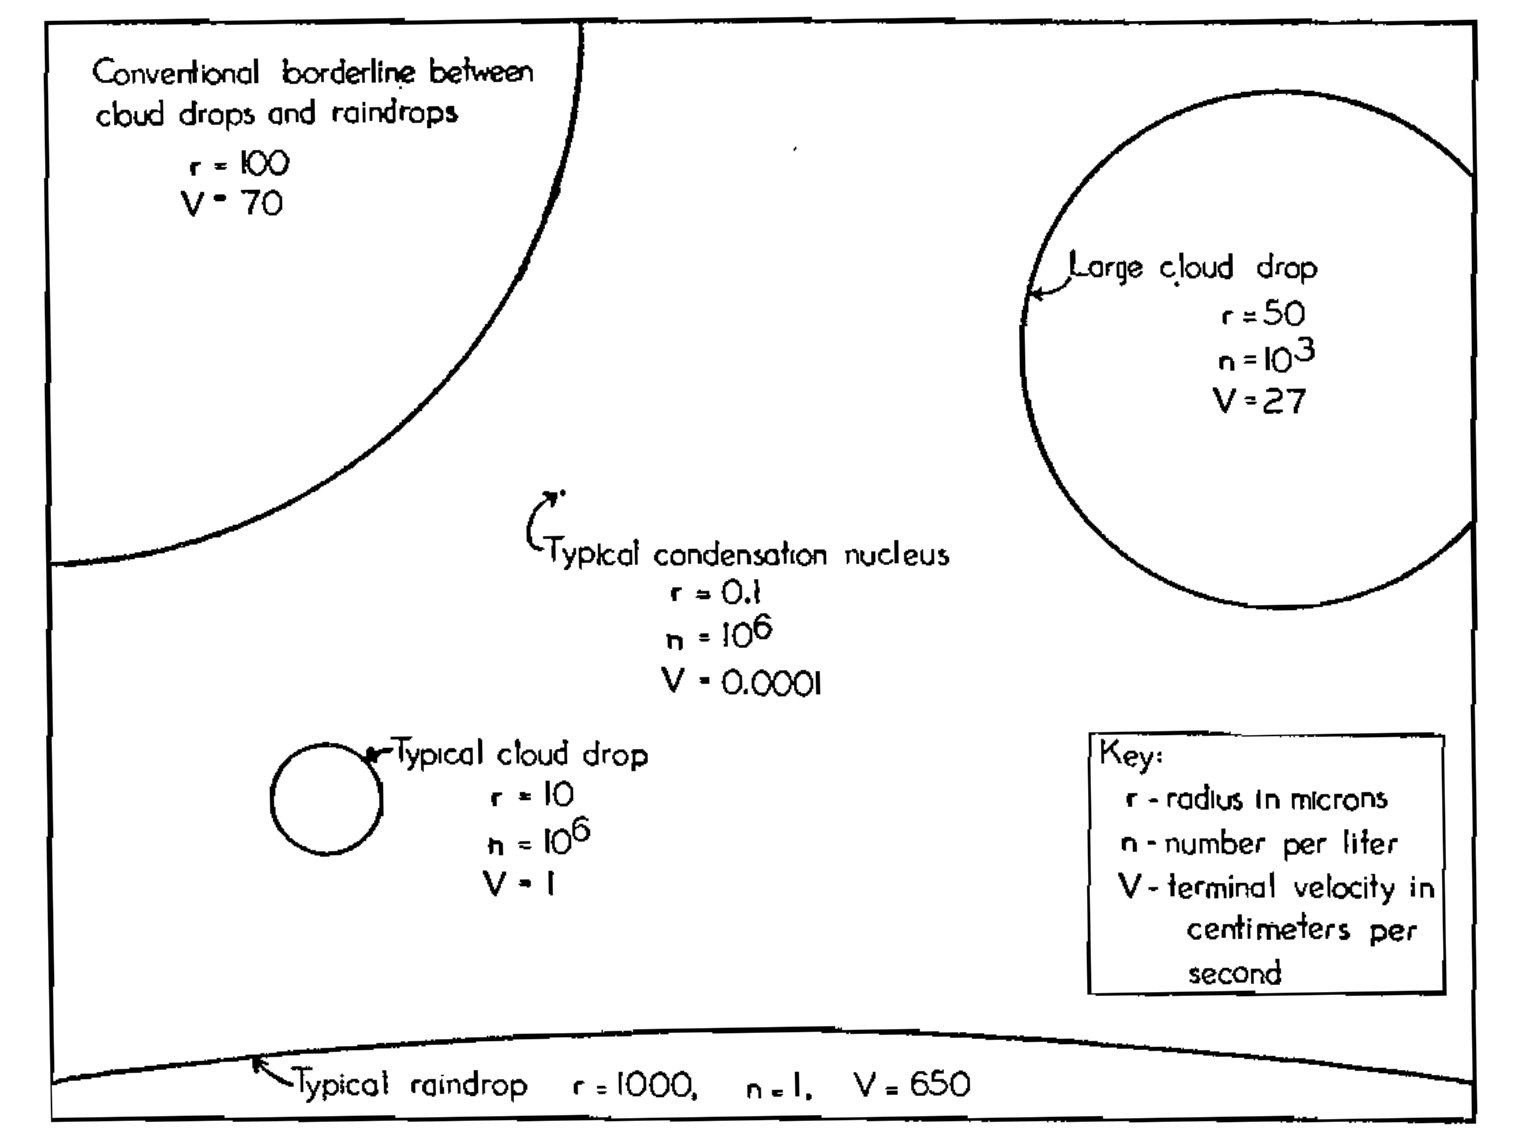
\includegraphics[width=1\textwidth]{dropletsize.png}
\caption{Size of CCN, typical cloud droplet, large cloud droplet, boarderline between cloud droplets and raindrops and typical size of raindrop. Adapted from~\citep{McDonald1958}.}
\label{fig:Schf01}
\end{figure}
 
\section{Radiation and clouds}
The cloud microphysical properties that determine the cloud radiative properties include: the amount of condensed water, the size and shape of the cloud particles, and the phase of the particles/and if the particles are liquid or ice~\citep{Curry1996}. The amount of condensed water can be expressed by the liquid water content (LWC) in the cloud, often presented with units $g~m^{-3}$, and is proportional to the median volume radius, $\overline{r}$, $\mju~m$. From~\cite{Rogers1989} we can express the number of droplets with radius $r$ by
\begin{equation}
N = \int n(r) dr
\end{equation}
where $N$ is the droplet number concentration $cm^{-3}$, and $n(r)$ is the number of droplets with radius $r$. @isit?
The LWC can be written
\begin{eqnarray}
LWC &=& \int \rho_L \frac{4}{3} \pi r^3 n(r) dr\\
&=& \frac{4}{3} \pi \rho_L \int r^3 n(r) dr\\
&=& \frac{4}{3} \pi \rho_L \overline{r}^3 \int n(r) dr\\
&=& \frac{4}{3} \pi \rho_L \overline{r}^3 N 
\end{eqnarray}
where the last equation shows the proportionality of LWC to the droplet number concentration $N$, and $\rho_L$ is the density of liquid water.

If the LWC is integrated over the height of the cloud, or any layer with chosen base and top in the atmosphere, we find the liquid water path (LWP) of that layer.
\begin{equation}
LWP = \int_{base}^{top} LWC dz
\end{equation}
The LWP is the column of liquid water in a cloud and is usually expressed by $g~m^{-2}$.


The cloud droplet effective radius determines many important radiative properties of a cloud and is therefore of particular interest. For example it determines the cloud albedo~\citep{Hansen1974}, which I will go more into when describing the first indirect effect.



Cloud consist of droplets that absorb and scatter SW radiation and absorb, scatter and emit LW radiation.. 
(introduction@)In this thesis shortwave (SW) radiation means solar radiation and longwave (LW) radiation covers the terrestrial infrared radiation.
How clouds scatter and absorb SW and LW radiation.
Explain something about blackbodies, clouds and blackbodies? Stefan–Boltzmanns law states that the flux density emitted by a blackbody is proportional to the fourth power of the absolute temperature @citeLiou2002page12. For a greybody, like a cloud, the equation can be written
\begin{equation}
F = \epsilon \sigma T^4
\end{equation}
where the emissivity of the greybody, $\epsilon$, is included. $F [W~m^{-2}]$ is the flux density emitted by the greybody, and $\sigma = 5.67\cdot 10^{-8} Jm^{-2}sec^{-1}deg^{-4}$ is the Stefan–Boltzmann constant.


Write about optical depth from Wallace and Hobbs: Normal optical depth or optical thickness, $\tau_{\lambda}$ is a measure of the cumulative depletion that a beam of radiation directed straight downward (zenith angle $\theta = 0$) would experience in passing through a defined layer \citep{WallaceHobbs2006}. The optical depth can be expressed as
\begin{equation}
\tau_{\lambda} = \int_z^{\infty} k_{\lambda} \rho r dz
\end{equation}
where $k_{\lambda}$ is the mass absorption coefficient, which has units of $m^2~kg^{-1}$, $\rho$ is the density of air, which has units of $kg~m^{-3}$, and $r$ is the mass of the absorbing gas per unit mass of air.



As mentioned in Chapter~\ref{chap:introduction} Introduction there is no solar radiation to reflect during winter and the polar night in the Arctic, where as in the summer the zenith angle is so high that even though there is sunlight 24 hours a day the cooling effect in summer does not average out the heating effect the clouds have in winter. The low clouds' ability to absorb and emit terrestrial radiation domiantes over their reflective effect on the solar radiation. @cite?

How do clouds reflect radiation? What is the effect of more water? Or more ice? What about the droplet size? (effective radius)\\
How do clouds absorb and emit radiation? Effect of more or less water or ice? Droplet size?

Ice is more effective in reflecting SW than water. Snow has a higher albedo than rain. Is there any use in presenting some albedo values for water, snow, ice? Or open water versus sea ice? New ice versus old sea ice?

Make sure to include something on how LWC/LWP and effective radii plays in, if this is to be mentioned in the results or discussion!!

\section{Aerosol effects on clouds}
Aerosols affect clouds in numerous ways. They have a direct effect on the climate by scattering and absorbing SW radiation. acting as CCNs og INs. elaborate?
If there are few CCNs a cloud in the area would be a clean cloud with few, but large droplets and therefore have a low albedo and precipitate easily. If the area had high aerosol concentration, the cloud would be polluted and have more numerous but smaller droplet, which means it would have a higher albedo and precipitation woul be suppressed. 

Not only the aerosol burden is important, if it is the same for two areas with different meteorological forcing that would also affect the cloud properties. Say an area has weaker updraft than another area, a cloud formed due to the weaker updraft will have lower LWC, lower albedo and little precipitation. The cloud formed in a stronger updraft will have higher LWC, higher albedo and be more precipitating.

@introduction?---
Diminishing sea ice could lead to an increase in the aerosol number concentrations in the area where ice has retreated. The open sea surface it self would lead to an increase in release of sea salt to the lower atmosphere @cite. The lack of sea ice would also increase the likelyhood that the sea could be used for shipping, which would pollute the area @cite.
----
There are two known indirect effects that aerosols have on radiation, through clouds. The first indirect effect was proposed by~\cite{Twomey1974} and is some times referred to as the Twomey effect. The second indirect effect was proposed by~\cite{Albrecht1989} @citecorrectly 

\subsection{The first indirect effect} (Maybe just call it all indirect effects and refer to Lohmann and Feichter)
The first indirect effect, suggested by~\cite{Twomey1974}, describes the enhancement of cloud albedo as a consequence of an increase in aerosol content and thereby available CCNs.
In short, the first indirect effect is a cloud albedo enhancement.
By increasing droplet concentration and hence the optical thickness of a cloud, pollution acts to increase the reflectance of clouds~\citep{Twomey1977}. 
The optical thickness is increased when the number of CCN is increased. Although the changes are small, the long term effects on climate can be profound~\citep{Twomey1974}.

Meg: The optical depth will change with changes in aerosol number concentrations and changes in clouds and their properties. For instance if a cloud has many small droplets, the optical depth will be higher. Where as  fewer cloud droplets will yield a lower optical depth, resulting in more SW radiation reaching the ground — possibly having a warming effect on the area. 


\subsection{The second indirect effect}
Albrecht 1989 
The second indirect effect, or the cloud lifetime effect, suggests more numerous but smaller droplets reduce the precipitation efficiency and by that enhances the cloud lifetime and hence the cloud reflectivity~\citep{Albrecht1989}. This effect has been estimated to be of roughly as large as the first indirect effect~\citep{Lohmann2005}.


Production of DMS by phytoplankton Charlson 1987


 %theory
\chapter{Model and methods}
\label{chap:modmet}
To test the thesis hypothesis, a formulation of the Weather Research and Forecasting (WRF) Model called the Advanced Research WRF (ARW) has been used. The model is described in the first part of this chapter. Then follows a description of the model setup and the different physics schemes that were chosen for this study, before a summary of the different runs that were performed. Ending the chapter are two short sections on the input data and processing of the model output.

%---------------------
\section{Description of the WRF-ARW Modeling System}
\label{sec:modeldes}
%---------------------
The version of the WRF-ARW modeling system used is 3.6.1, which was released in April 2014. The model is primarily developed at the National Centre for Atmospheric Research (NCAR) in Boulder, Colorado. The ARW model is the first fully compressible conservative form nonhydrostatic model designed for both research and operational numerical weather prediction (NWP) applications~\citep{Skamarock2008}. 

As can be seen from figure~\ref{fig:wrfflowchart} the WRF-ARW Modeling System consists of four major programs~\citep{Wang2015}:
\begin{itemize}
\item The WRF Preprocessing System (WPS)
\item WRF-Data Assimilation (WRF-DA)
\item ARW solver
\item Post-processing \& Visualization tools
\end{itemize}

\begin{figure}[ht]
\centering
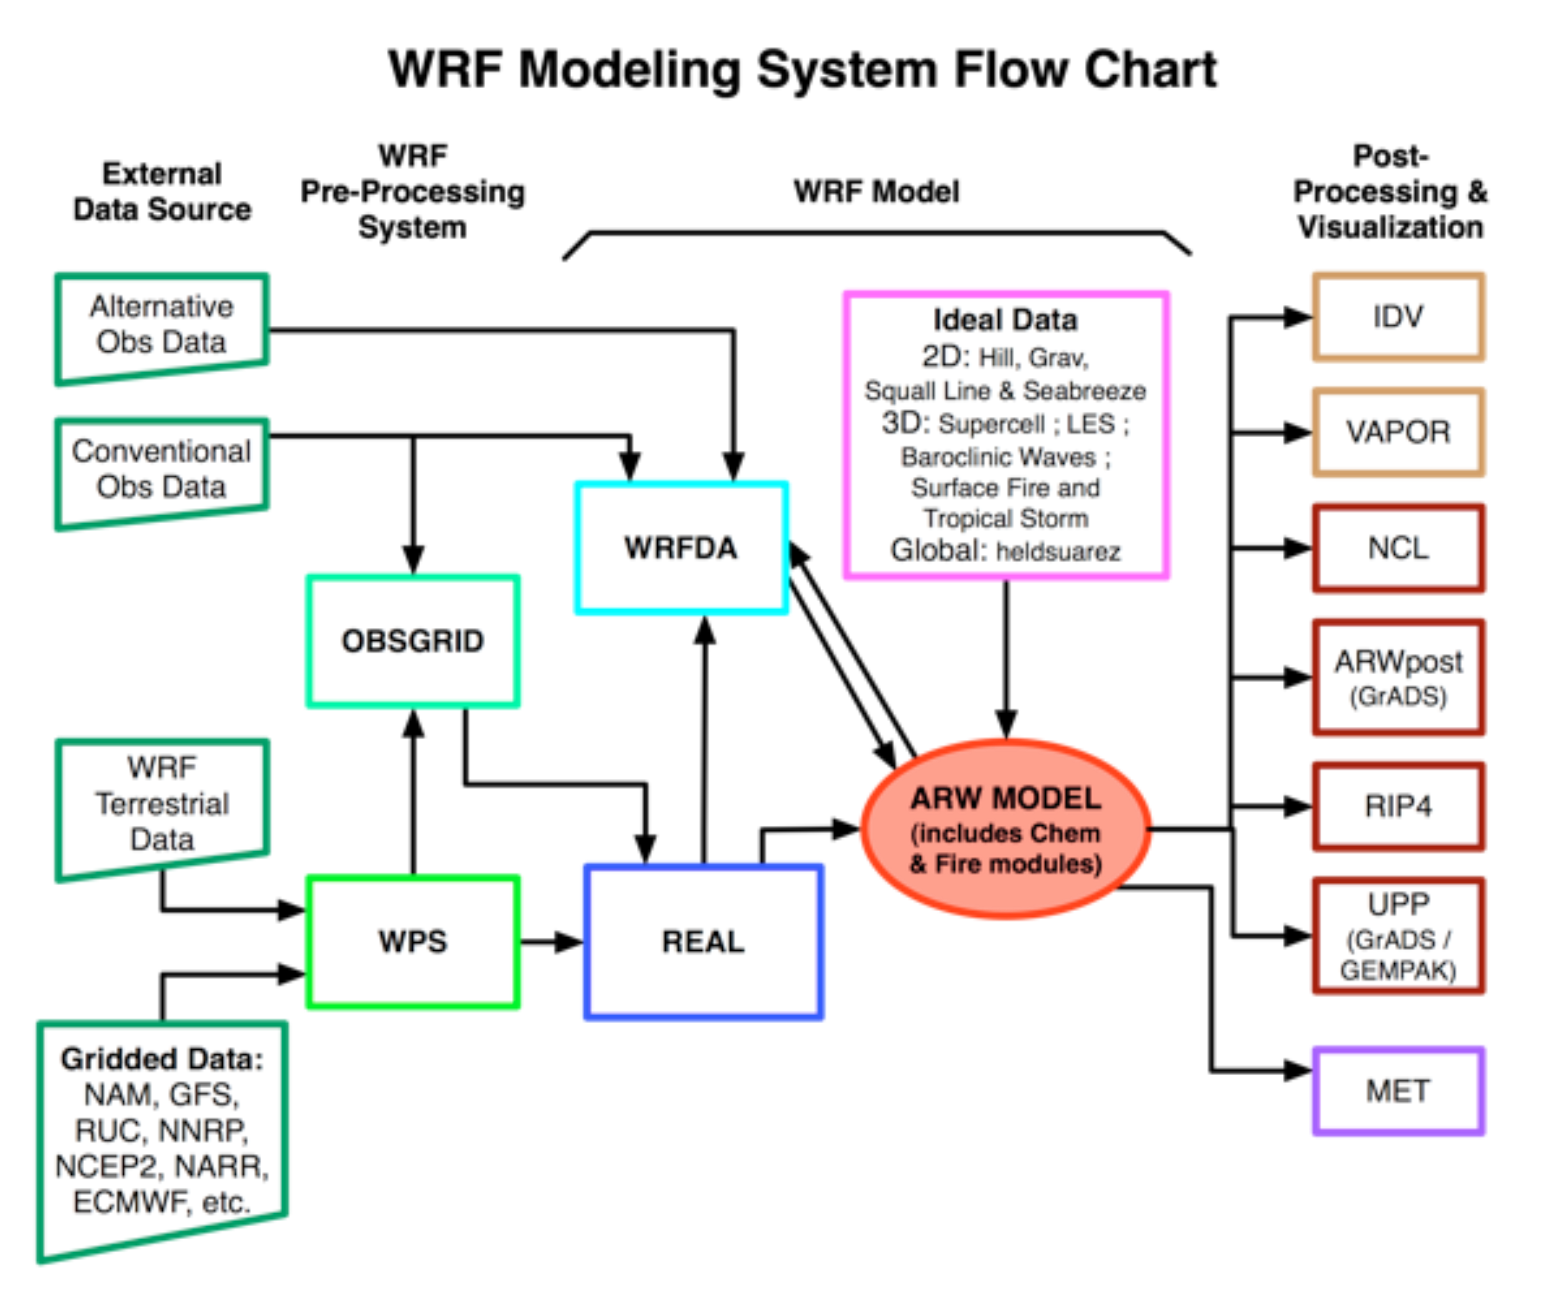
\includegraphics[width=0.9\textwidth]{model_methods/wrfflowchart}
\caption{Flowchart for the WRF ARW Modeling System Version 3. From~\citet{Wang2015}.}
\label{fig:wrfflowchart}
\end{figure}

WPS is used primarily for real data simulations~\citep{Wang2015}, like the study presented in this thesis. A real-data simulation means that it has been initialized by observations and reanalysis, not artificial data. WPS' functions include defining simulation domains, interpolating terrestrial data and degribbing and interpolating meteorological data from another model to this simulation domain~\citep{Wang2015}. WRF-DA is optional and can be used to ingest observations into the interpolated analyses created by WPS~\citep{Wang2015}, but was not used in this study. The ARW solver is the key component of the modeling system, which is composed of several initialization programs for idealized, and real-data simulations, and the numerical integration program~\citep{Wang2015}.% Fully compressible nonhydrostatic equations with hydrostatic options, regional and global applications, complete coriolis and curvature terms and that vertical grid-spacing can vary with height are among the WRF models key features according to~\citet{Wang2015}.

The continuous equations solved in the ARW model are the Euler equations cast in a flux form where the vertical coordinate, $\eta$, is defined by a normalized hydrostatic pressure,
\begin{equation}
\eta = (p_h - p_{ht})/\mu 
\end{equation}
where $\mu = (p_{hs} - p_{ht})$~\citep{Skamarock2008}. $p_h$ is the hydrostatic component of the pressure and $p_{hs}$ and $p_{ht}$ are the values of the hydrostatic pressure in a dry atmosphere at the surface and top boundaries respectively~\citep{Skamarock2008}.

The vertical coordinate is the traditional $\sigma$ coordinate used in many hydrostatic atmospheric models, but is denoted by $\eta$ in ARW, and is shown in figure~\ref{fig:sigma}.

\begin{figure}[ht]
\centering
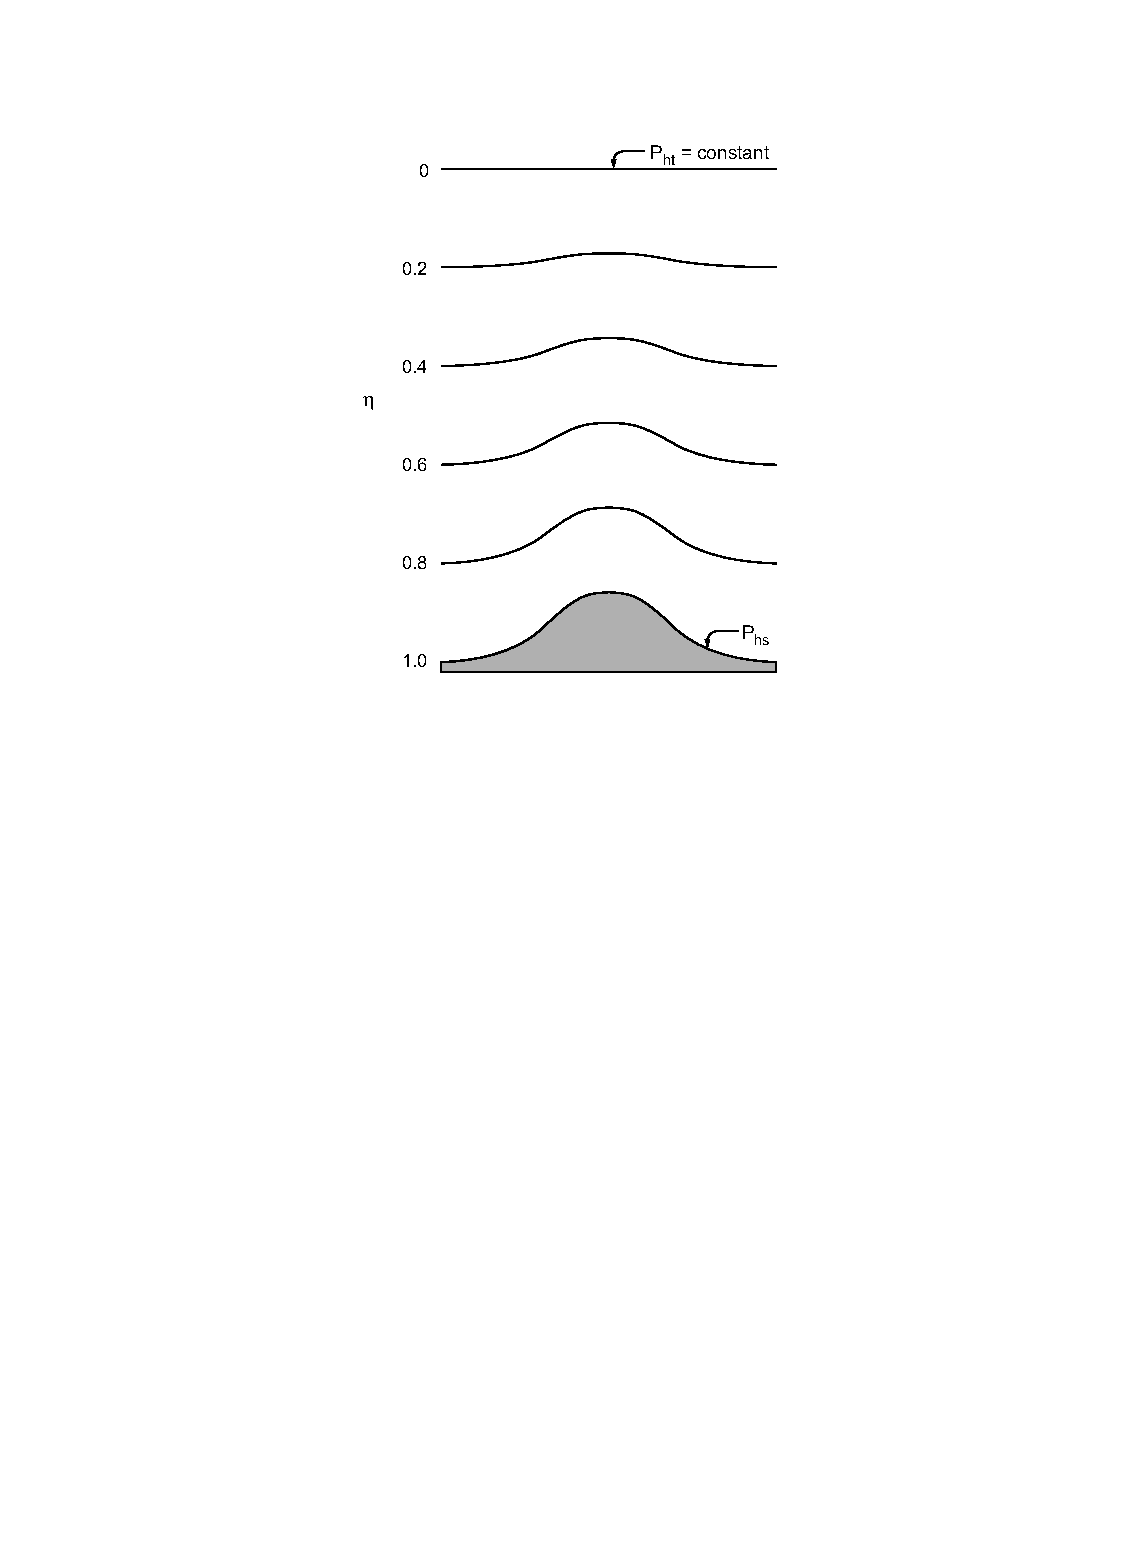
\includegraphics[scale=0.9]{model_methods/sigma.pdf}
\caption{This figure is shown as presented in~\citet{Skamarock2008}, and is a schematic of the $\eta$ coordinate. $P_{hs}$ and $P_{ht}$ represent the hydrostatic pressure at the surface and top respectively.}
\label{fig:sigma}
\end{figure}

$\eta$ decreases monotonically from a value of 1 at the surface, where the coordinate follows the terrain and $P_h = P_{hs}$, to a value of 0 at the top level, which is then a pressure surface, where $P_h = P_{ht}$. Levels with constant $\eta$ are commonly referred to as $\eta$-levels (or Eta-levels). $\mu(x,y)$ is the mass of dry air per unit area within the column in the model domain at $(x,y)$. The $\eta$-levels are where the vertical wind speed is calculated, whereas the thermodynamic variables ($\theta$) are calculated between the $\eta$-levels, on so-called mass levels.

%--------- Stuff on staggered grid.
With the vertical coordinate $\eta$, and the mass of an air column, $\mu(x,y)$, in the model grid the Euler equations can be written with  variables on flux form:
\begin{eqnarray*}
\textbf{V} = \mu \textbf{v} = (U,V,W),\textit{    }\Omega = \mu \dot{\eta},\textit{    }\Theta = \mu \theta
\end{eqnarray*}
Now \textbf{v} is the velocity vector in three dimensions, $\omega = \dot{\eta}$ denotes the vertical velocity and $\phi$ is the geopotential, and the set of prognostic equations that needs to be solved numerically is this:
\begin{eqnarray}
\partial_t U + (\nabla \cdot \textbf{V}_u) - \partial_x (p\phi_{\eta}) + \partial_{\eta}(p\phi_x) &=& F_U\\ \label{eqn:euler1}
\partial_t V + (\nabla \cdot \textbf{V}_v) - \partial_y (p\phi_{\eta}) + \partial_{\eta}(p\phi_y) &=& F_V\\
\partial_t W + (\nabla \cdot \textbf{V}_w) + g(\partial_{\eta}p-\mu)&=&F_W\\
\partial_t \Theta + (\nabla \cdot \textbf{V}\theta) &=& F_{\Theta}\\ \label{eqn:euler2}
\partial_t \mu + (\nabla \cdot \textbf{V}) &=& 0\\
\partial_t \phi + \mu^{-1}[(\textbf{V} \cdot \nabla \phi - gW) &=& 0\\
\partial_t Q_m + (\nabla \cdot \textbf{V}Q_m) &=& F_{Q_m} \label{eqn:euler3}
\end{eqnarray}
To close the system they use the diagnostic equation for inverse density, $\alpha_d$,
\begin{equation}
\partial_{\eta} \phi = -\alpha_d \mu
\end{equation}
and the moist equation of state
\begin{equation}
p = p_0\left(R_d\theta\frac{1+R_d/R_v)q_v}{p_0\alpha_d}\right)^{\gamma}
\end{equation}
where $\gamma = c_v/c_p = 1.4$ is the ratio of the heat capacity for dry air at constant volume, to that of constant pressure, $R_d$ and $R_v$ are the gas constants for dry and moist air respectively, $q_v$ is the mixing ratio of water vapor and $p_0$ is the reference pressure (10$^3$hPa). The right-hand-side terms in equations~\ref{eqn:euler1}-\ref{eqn:euler2} and~\ref{eqn:euler3} represent forcing terms which arise from model physics, turbulent mixing, spherical projections, the earth's rotation, and moist physics~\citep{Skamarock2008a}.

To solve these equations the WRF-ARW modeling system uses the spatial discretization known as a staggered C grid~\citep{Skamarock2008a}. Figure~\ref{fig:stagger} shows the schematic of the grid and how the velocities, $u$ and $v$, are calculated at the edges of each grid box both in the horizontal and in the vertical, half a grid box length away from the thermodynamic variable, which is calculated in the middle of each grid box, at the mass point. The advection in and out of the grid box is calculated from $u$ and $v$. This staggering allows for discretization of the pressure gradient and divergence terms across a single grid interval, without any averaging, which gives a highly accurate second order difference.

\begin{figure}[ht]
\centering
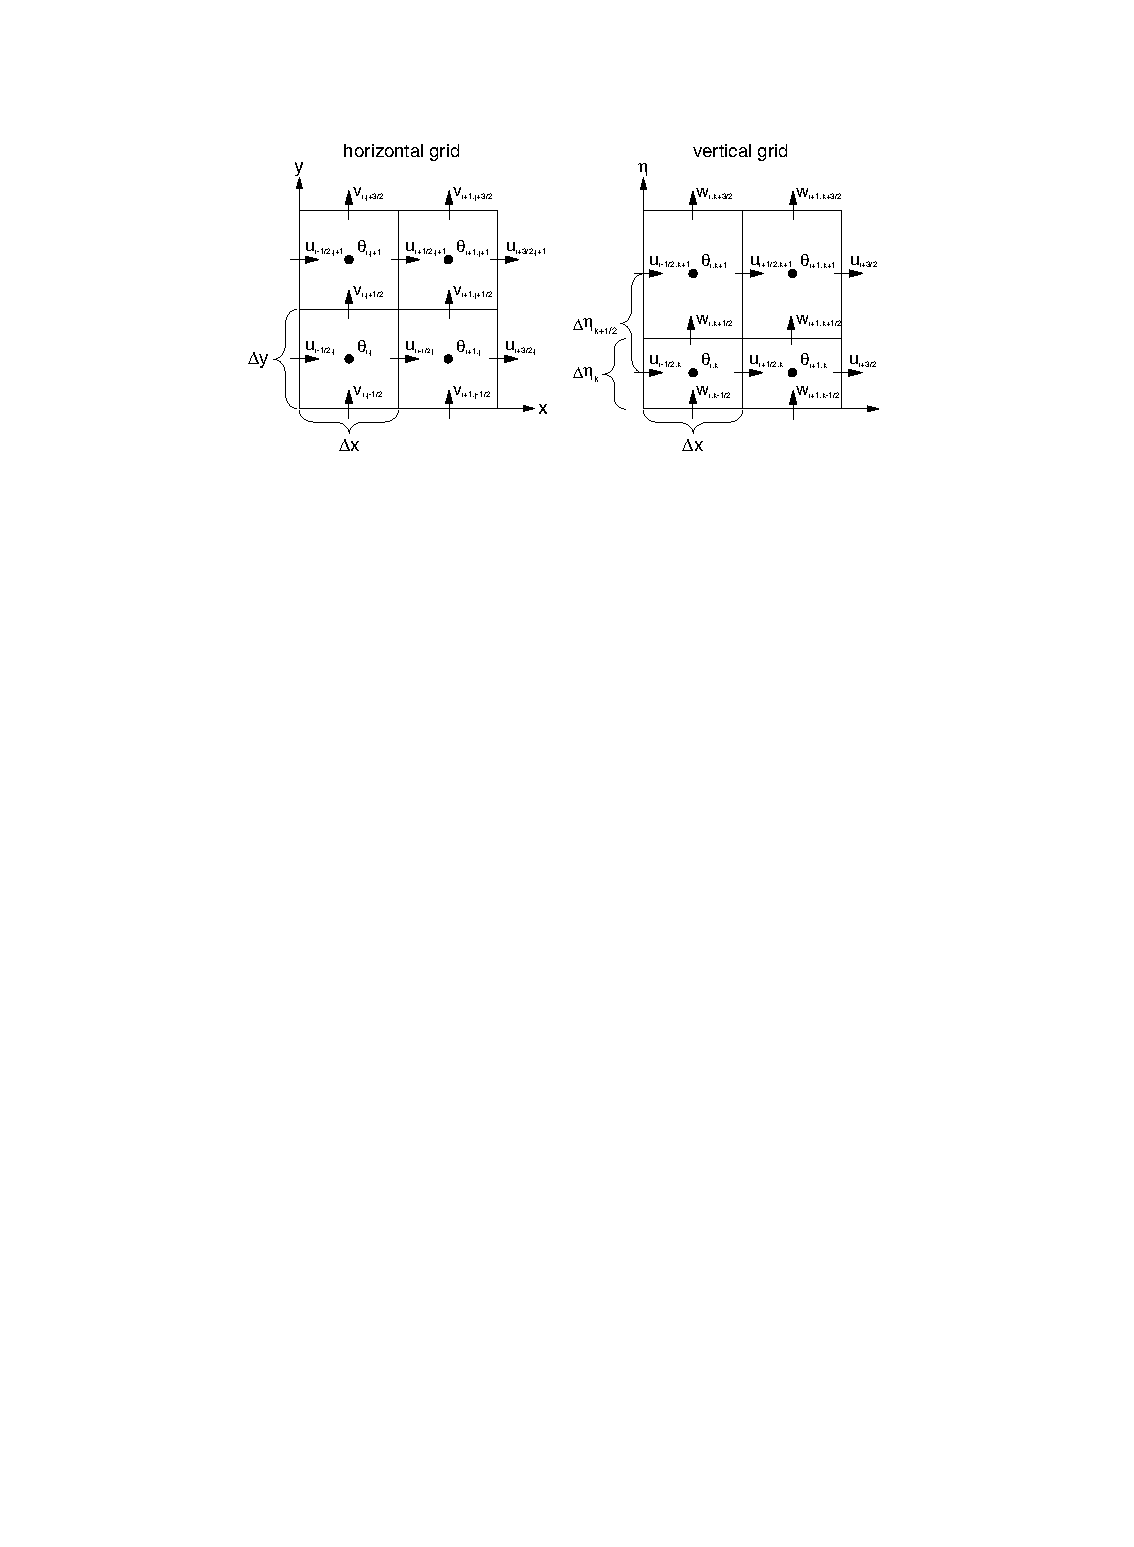
\includegraphics[width=\textwidth]{model_methods/gridstagger.pdf}
\caption{This figure is shown as presented in~\citet{Skamarock2008}, and shows the staggering of the C-grid. The horizontal staggering to the left, and the vertical staggering to the right.}
\label{fig:stagger}
\end{figure}

The time integration in ARW is performed by a "time split integration scheme", which means that the low frequency, meteorologically significant modes are integrated by a third order Runge-Kutta (RK3) integration scheme, while the higher frequency acoustic modes are integrated with a shorter time step, to conserve the numerical stability. In general, it is preferred to use as large a time step as possible while keeping the numerical stability. For integration by the RK3 scheme the maximum time step $\Delta t_{max}$ is found through equation~\ref{eqn:tmax}
\begin{equation}
\Delta t_{max} < \frac{C\cdot \Delta x}{\sqrt{3}\cdot u_{max}}
\label{eqn:tmax}
\end{equation}
where $C$ is the maximum Courant number, which depends on the order of the discretization of the advection terms. Typically in WRF, it is recommended that $\Delta t$ (in seconds) does not exceed 6 times $\Delta x$ (in km). When running the modeling system with a horizontal resolution of 4~km grid point spacing I therefore chose $\Delta t = 24$. Details about the model runs and choices of physics in the model is presented in the next section.

%---------------------
\section{Model setup}
\label{sec:modelsetup}
%---------------------
The model was ran with a 4~km$\times$4~km horizontal grid point spacing, with 300$\times$300 grid points, and 72 vertical layers, with the model top at 10~hPa.
The area covers parts of the Beaufort Sea, by Canada and Alaska. This area was chosen because data from the area has been used for related studies~\citep{Intrieri2002,Shupe2004,Kay2009,Wu2012,Palm2010,Schweiger2008} %@@@sjekk dette!!,
as mentioned in Chapter~\ref{chap:introduction}. The area is not completely ice free any part of the year~\citep{NSIDC}, and provides a good place to simulate cloud-sea ice interaction. The area is over several time zones but is approximately 7 hours behind UTC time. The times given in the WRF-ARW modeling system are UTC. The model was run for a period of 5~days, 1st to 6th of September 2012. This is approximately when the record low ice extent in the Arctic was set (eg. National Snow and Ice Data Centre, U.S.A.,~\citep{NSIDC}).

The vertical layers in the ARW model are often referred to as eta levels, because of the choice of $\eta$ as the vertical coordinate. These levels have uneven vertical spacing and the altitude of each level is dependent on pressure, therefore the level height varies in both time and space. As a consequence of pressure dependence, the levels in the lower troposphere are closer to each other than the levels higher up in the troposphere. Thus the low clouds in the area can be resolved. Approximate heights for the lowest 11 eta levels are shown in Table~\ref{tab:etaheights}.

\begin{table}[H]
\centering
\caption{Approximate height for each level in meters above the surface.}
\label{tab:etaheights} 
\begin{tabular}{C{4.cm} C{5.cm}}
\centering
\textbf{Eta level} & \textbf{Approximate height}\\ \hline
1 & 10~m\\
2 & 50~m\\
3 & 130~m\\
4 & 230~m\\
5 & 370~m\\
6 & 530~m\\
7 & 650~m\\
8 & 950~m\\
9 & 1250~m\\
10 & 1400~m\\
11 & 1600~m
\end{tabular}
\end{table}

%------------------------------------------
\subsection{Choices of physics in the model}
%------------------------------------------
The selection of physics schemes in WRF-ARW are numerous and fall into several categories, each containing several choices. Table~\ref{tab:physics} shows some of the different categories and the choice of scheme, for this study, within each of those categories.

\begin{table}[H]
\centering
\caption{Table of physics categories and choice of scheme for this thesis}
\label{tab:physics} 
\begin{tabular}{L{4cm} L{7cm}}
\centering
\textbf{Physics categories} & \textbf{Scheme selected within category}\\ \hline
(1) microphysics & aerorol-aware ~\citep{Reisner1998, Thompson2004, Thompson2008, Thompson2014}. Option 28.\\
(2) cumulus parameterization & Grell 3D  @cite authors. Option 5.\\
(3) planetary boundary layer (PBL) &  Yonsei University scheme @cite authors. Option 1.\\
(4) land-surface model & Noah Land Surface Model @cite authors. Option 2.\\
(5) radiation & RRTMG LW \& SW ~\citep{Mlawer1997, Iacono2000, Iacono2003, Iacono2008}. Radiation option 4 in both LW and SW.
\end{tabular}
\end{table}

The ARW model offers a wide selection of schemes to treat different physics that one wants represented in the model. The schemes treat the physics slightly differently and some schemes are better for certain horisontal and vertical resolutions than others, so one needs to be careful when choosing how the model is to treat the physics. For my thesis, the especially relevant scheme to mention is the cloud microphysics scheme that I chose, which is the aerosol-aware scheme described in~\citet{Thompson2014}. When studying cloud and radiation response to removal of sea ice one might expect an increase in aerosols from the open ocean and increased sea traffic. The aerosols are therefore also relevant for the choice of schemes, and the aerosol-aware scheme, described further below, includes the necessary processes for this study.

The choice of cumulus parameterization was based on the grid resolution, and the best fit for it. A horizontal grid point spacing of 4~km can be fine enough to not use cumulus parameterization~\citep{Thompson2014}, but in this thesis a parameterization that was more suitable for grid point spacings less than 10~km was chosen; the Grell 3D parameterization. According to~\citet{Wang2015} Grell 3D may be used on high resolution, like my 4~km grid point spacing.
%---------
%Yonsei University scheme was chosen for the PBL. It is a non-local-K scheme with explicit entrainment layer and parabolic profile in unstable mixed layer~\citep{Wang2015}.
%---------
%The land-surface model choice came to Noah Land Surface Model. The Noah Land Surface Model, is a unified NCEP/NCAR/AFWA (National Centers for Environmental Prediction, National Centre for Atmospheric Research, Air Force Weather Agency) scheme with soil temperature and moisture in four layers which provides sensible and latent heat fluxes to the PBL scheme~\citep{Wang2015}. Additionally, it predicts soil ice, and fractional snow cover effects, which could be important in the Arctic, but it is probably not the most important choice, since there is very little land in the area investigated, see figure~\ref{fig:area} in Chapter~\ref{chap:introduction}.
%----------
%The radiation schemes were chosen simply because they are the best match for the microphysics scheme at the time of writing. According to~\citet{Thompson2014} the Rapid Radiative Transfer Model (RRTM) for General Circulation Models (GCMs) (RRTMG) schemes for SW and LW are the only radiation schemes which include the effects of the effective radii calculated in aerosol-aware. The RRTMG schemes are accurate schemes using look-up tables for efficiency, and accounts for multiple bands and microphysics species, and includes the Monte Carlo Independent Column Approximation (MCICA) method of random cloud overlap~\citep{Wang2015}.

%------------------------------------------
\subsubsection{The aerosol-aware scheme}
%------------------------------------------
The microphysics includes explicitly resolved water vapor, cloud, and precipitation processes. The aerosol-aware scheme was chosen so that the study would have scavenging of aerosols included and have proper enough representation of aerosols to study aerosol-cloud interactions, without using the WRF model coupled with chemistry (WRF-Chem).
According to the ARW User's Guide by~\citet{Wang2015}, the aerosol-aware scheme considers water- and ice-friendly aerosols, and a climatological dataset may be used to specify initial and boundary conditions for the aerosol variables. I have used this climatological dataset, which will be explained in Subsection~\ref{subsec:inputdata}~Input~data. The scheme uses a monthly mean for aerosol number concentrations derived from multi-year (2001-2007) global model simulations in which particles and their precursors are emitted by natural and anthropogenic sources and are explicitly modeled with multiple size bins for multiple species of aerosols by the Goddard Chemistry Aerosol Radiation and Transport (GOCART) model %(@desiterteGinoux2001)
~\citep{Thompson2014}.
The aerosol-aware scheme~\citep{Thompson2014} is built on the schematic shown in figure~\ref{fig:microphysics}, from~\citet{Reisner1998}. It is a double moment scheme, which means it computes both mass mixing ratios, Q, and number concentrations, N, for the same water species (hydrometeors). 

\begin{figure}[h]
\centering
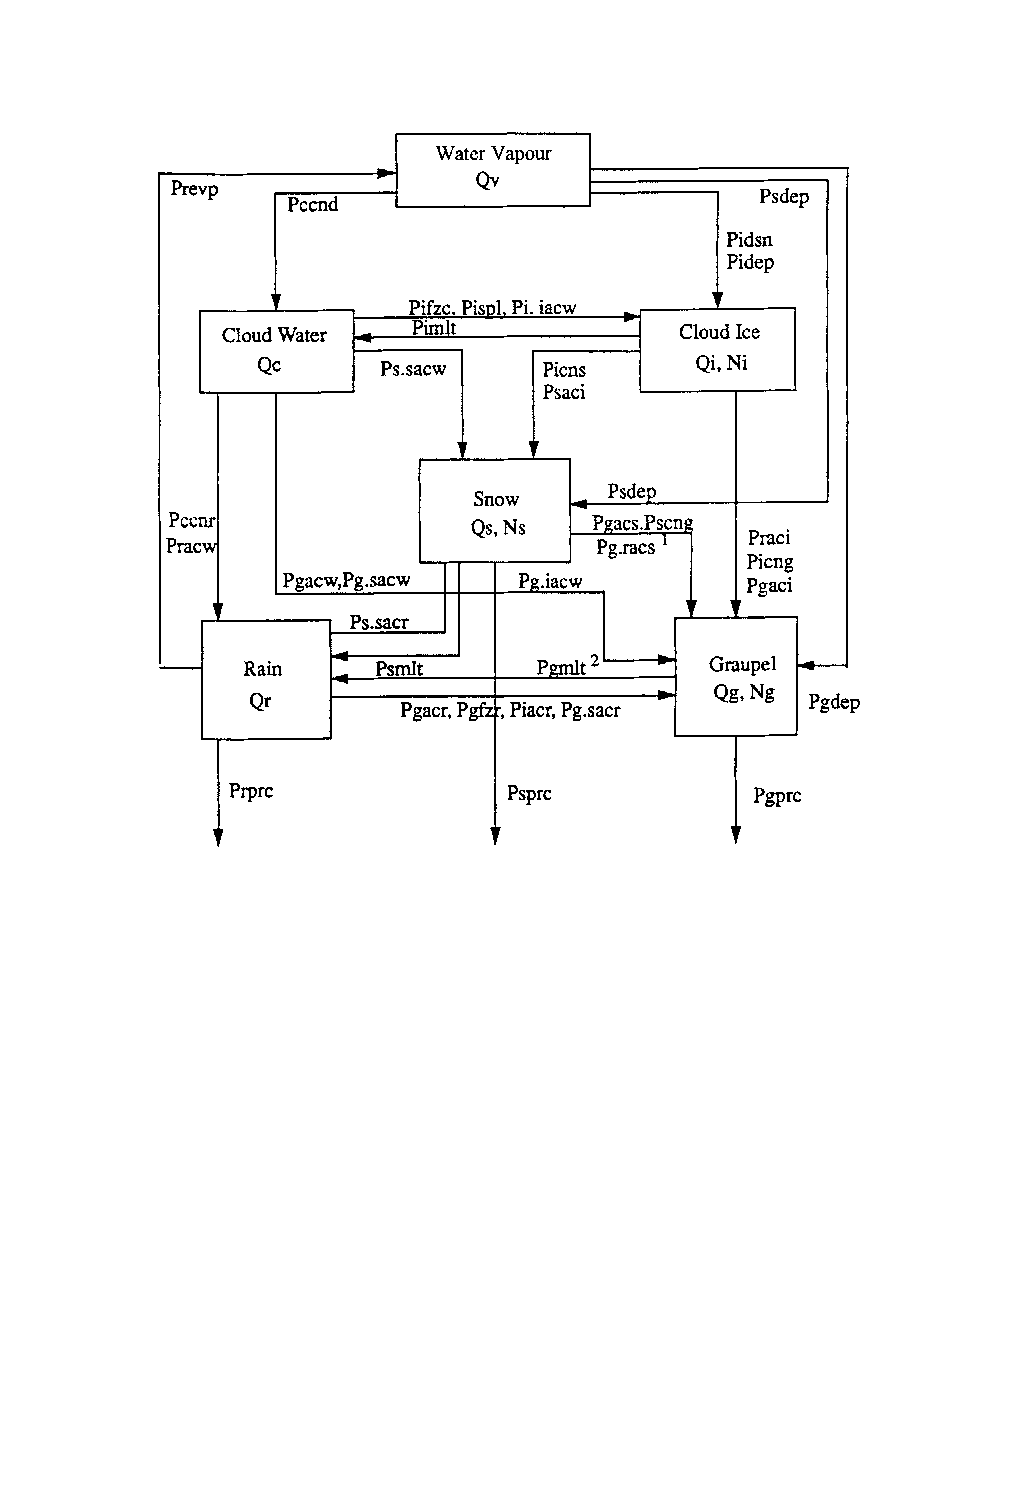
\includegraphics[width=0.9\textwidth]{model_methods/microphysics.pdf}
\caption{Cloud microphysical parameterization scheme used in some NWP models as shown in~\citet{Reisner1998}. A full list of the acronyms used in the schematic can be found in~\citet{Reisner1998}.}
\label{fig:microphysics}
\end{figure}

Figure~\ref{fig:microphysics} show the processes in the microphysics scheme developed by~\citet{Reisner1998}, which the first bulk microphysics scheme by Thompson~\citep{Thompson2004} was based on. The aerosol-aware scheme~\citep{Thompson2014} is an extension of the updated Thompson bulk microphysics scheme described in~\citet{Thompson2008}. The figure shows a schematic of five hydrometeors, cloud water (c), rain (r), ice (i), snow (s) and graupel (g), and if just the mass mixing ratio is calculated or if both the mass mixing ratio and the number concentration is calculated. For each of the hydrometeors, prognostic equations are used with all the sources and sink terms included.
 % which was originally built on this~\citep{Thompson2004}, but there is not much left of it in the code now (@cite the code comments?).
 
%------------------------------------------
\subsubsection{The RRTMG radiation schemes}
%------------------------------------------
According to~\citet{Thompson2014} the Rapid Radiative Transfer Model (RRTM) for General Circulation Models (GCMs) (RRTMG) schemes for SW and LW~\citep{Mlawer1997, Iacono2000, Iacono2003, Iacono2008} are the only radiation schemes which include the effects of the effective radii calculated in aerosol-aware. These were therefore used in combination with the aerosol-aware cloud microphysics scheme. The RRTMG schemes are accurate schemes using look-up tables for efficiency, and accounts for multiple bands and microphysics species, and includes the Monte Carlo Independent Column Approximation (MCICA) method of random cloud overlap~\citep{Wang2015}.
%The RRTM scheme described in~\citet{Mlawer1997} uses the correlated-k method, which is an approximated technique for the accelerated calculation of fluxes and cooling rates for inhomogeneous atmospheres~\citep{Mlawer1997}. %\textbf{@define inhomogeneous atmosphere}.
%The correlated-k method is capable of achieving accuracy comparable with that of line-by-line models with an extreme reduction in the number of radiative transfer operations performed~\citep{Mlawer1997}, which by that reduces computational cost and increases computational efficiency. The Line-By-Line Radiative Transfer Model (LBLRTM) is used both to calculate the absorption coefficients used to generate the k distributions needed by RRTM and  to evaluate the RRTM calculations of fluxes and cooling rates~\citep{Iacono2000}. 

%---------------------
\section{Model runs}
%---------------------
The results presented in the next chapter are based on four different runs. The control run is the run where the aerosol climatological dataset has been used unchanged, and where the sea ice is kept as it was in the downloaded input data, see Subsection~\ref{subsec:inputdata}. The control run is used as a base to compare the other runs to, those with no ice and/or increased aerosol number concentrations.

There are two runs where the sea ice was removed, NoIce and Aero10NoIce. The point of this is to compare the run with no ice to the control run, and see if there are any changes in the cloud properties, and SW and LW fluxes. For one of those runs the aerosol number concentration was also increased, results from this run can be compared with the control run.

The number of water- and ice-friendly aerosols were multiplied by 10 both with and without sea ice for two runs: Aero10 with ice, and as mentioned above, Aero10NoIce without ice. The goal is to find changes in cloud properties, and radiation fluxes compared to those in the control run.

Table~\ref{tab:runs} shows an overview of the different runs that have been executed, whose output have been used for production of figures presented in the next chapter.

\begin{table}[H]
\centering
\caption{Table showing the names of the runs and if they have sea ice or not, and if the aerosol concentration has been increased by a factor of 10 through input files. All the runs have the same horizontal resolution of 4~km$\times$4~km, dimensions 300$\times$300, 72 vertical layers and $\Delta t$=24~s.}
\label{tab:runs} 
\begin{tabular}{L{2.3cm} L{2cm} L{3cm}}
\centering
Name & Sea ice & Aerosol concentration\\ \hline
control & initial & climatology\\
NoIce & removed & climatology\\
Aero10 & initial & climatology$\times$10\\
Aero10NoIce & removed & climatology$\times$10\\
\end{tabular}
\end{table}

%---------------------
\subsection{Input data}
\label{subsec:inputdata}
%---------------------
The model runs were initialized with data downloaded from the European Centre for Medium-Range Weather Forecasts (ECMWF). %~\citet{ecmwf}
%@cite web page.%was downloaded from their site and used as input for initial and boundary?? conditions.
The downloaded data is from the ERA-Interim data set, which is a global atmospheric reanalysis from 1979 to present and continues to be updated in real time. %~\citet{ecmwf}.%@make bib for ecmwf
Through WPS the data from ERA-Interim was interpolated over the area, with a 2 degree minute spacing between the points, to be used to initialize the model. The data used is in 6-hourly atmospheric fields on pressure levels, for the first five days of September 2012, which was the period the model was run for. This is done to make sure the initial meteorological conditions are the same in every run, so that the effects of changing a variable in the input files for the modeling system are only due to that change.

To use the climatological aerosol data set, the file containing monthly means had to be called through WPS. The aerosol input data includes mass mixing ratios of sulfates, sea salts, organic carbon, dust, and black carbon from a 7-yr simulation with 0.5$\degree$ longitude by 1.25$\degree$ latitude spacing~\citep{Thompson2014}.

\subsection{Manipulation of input files}
The input files for the ARW solver, created by WPS and REAL (see figure~\ref{fig:wrfflowchart}) were manipulated by use of the NetCDF Operator (NCO) tool ncap2. In these files the sea ice was removed for the runs without sea ice (NoIce and Aero10NoIce) and the aerosol number concentration from the climatological dataset was multiplied by 10 for the runs with increased aerosol number concentration (Aero10 and Aero10NoIce).

%---------------------
\section{Processing the model output}
%---------------------
Figures presented in my thesis, I made (unless other is stated) by use of NCL (National Center for Atmospheric Research (NCAR) Command Language). For the NCL scripts I found a lot of help and inspiration from the example scripts for WRF-users.% available at @(URL for examples).

The model output was stored as instantaneous values for every hour for each of the five days, from each of the four runs. 

To study the response in cloud radiative properties, all fields of interest were made into daily time averages, by use of NCL, in each run. Some fields vary only in horizontal space and in time (2-dimensional in space), and were simply added together and divided by the number of hours in that day. These fields are: SW and LW radiation down at the surface and up at TOA, latent heat (LH) and sensible heat (SH), temperature at the surface and at 2~m height and winds at 10~m height.

The cloud parameters, such as $r_e$ and CDNC, vary also in the vertical (3-dimensional in space) and have been averaged over the 11 lowermost layers (the lower $\sim$1600~m above the surface) and all hours of the day. Hence, the figures showing $r_e$ and CDNC over maps do not account for variations in the vertical.

The LWC on the other hand has not been averaged over the layers, but summarized into LWP. In each of the lowermost 11 layers the LWC has been multiplied with the thickness of the respective layer and then added in height to make the LWP.

The differences between two runs, presented in the next chapter, are daily time averaged differences. Where the difference has been calculated for every hour of the day, and then averaged in time. %model and methods
%\chapter{Results and discussion}
\label{chap:results}
In this chapter, the findings made in the thesis are presented. First a section on the model output from the control run (Control) is described, which is also used for comparison and reference in the following sections. The chapter mostly consists of a discussion of why there is a difference in certain cloud and radiation variables between NoIce and Control, and between Aero10 and Control. At the end, there is also a small section on the difference in the fields between Aero10NoIce and Control.

The discussion is based on daily time averaged differences between Control and the other runs. The results are discussed separately for NoIce, Aero10 and Aero10NoIce for days 1 and 5. Here day 1 represents the closest to an "off line" run, with near instantaneous changes in clouds due to ice removal or aerosol increase, whereas by day 5 the atmosphere has had some time to adjust to the changes that were implemented at the beginning of the first day of the run.

I also try to answer if these results show a warming or cooling effect and if there is reason to believe that changes in sea ice extent and aerosol concentration will further influence the sea ice extent.

%--------------------
\section{The control run}
%--------------------
Figure~\ref{fig:weather} shows the weather situation in the control run for days 1 and 5. The temperature at 2~m height is represented by red contour lines, and the wind direction and speed at 10~m height is shown by the 
wind barbs and their color. Day 1, figure~\ref{subfig:weather_cont_day1} shows weak northerly winds ($\sim$ 5~m/s) bringing cold air, -3$\degree$C (270~K), from the north over the sea ice, and the westerly winds over the ocean south of the sea ice bring moisture to the air over the sea ice which contributes to the low stratus in figure~\ref{subfig:cross_LWC_day1}. Figure~\ref{fig:sections} contains the vertical cross sections of LWC and IWC (and temperature) over the line shown in figure~\ref{subfig:cross_line}. The deeper clouds over the island in figure~\ref{subfig:cross_LWC_day1} have been formed due to orographic lifting, and the height of the "mountain" is $\sim$400~m according to the y-axis in the cross section, and the filled contours of terrain height in figure~\ref{subfig:cross_line}. The westerly winds over the sea ice, towards the mountain at $\sim$76$\degree$N and 112$\degree$W, increase in strength over the mountain. The air is brought to saturation as it is lifted over the mountain by the winds, and forms deeper clouds over the mountain with LWC of $\sim$0.1~$\text{g/m}^3$. From figure~\ref{subfig:cross_IWC_day1}, showing the ice water content (IWC) in the section, one can see that the thicker clouds over the mountain also contain ice in the upper part of the clouds, with about 5$\cdot\text{10}^{-3}$~$\text{mg/m}^3$. 

\begin{figure}
    \centering
    \begin{subfigure}{0.48\textwidth}
        \centering
        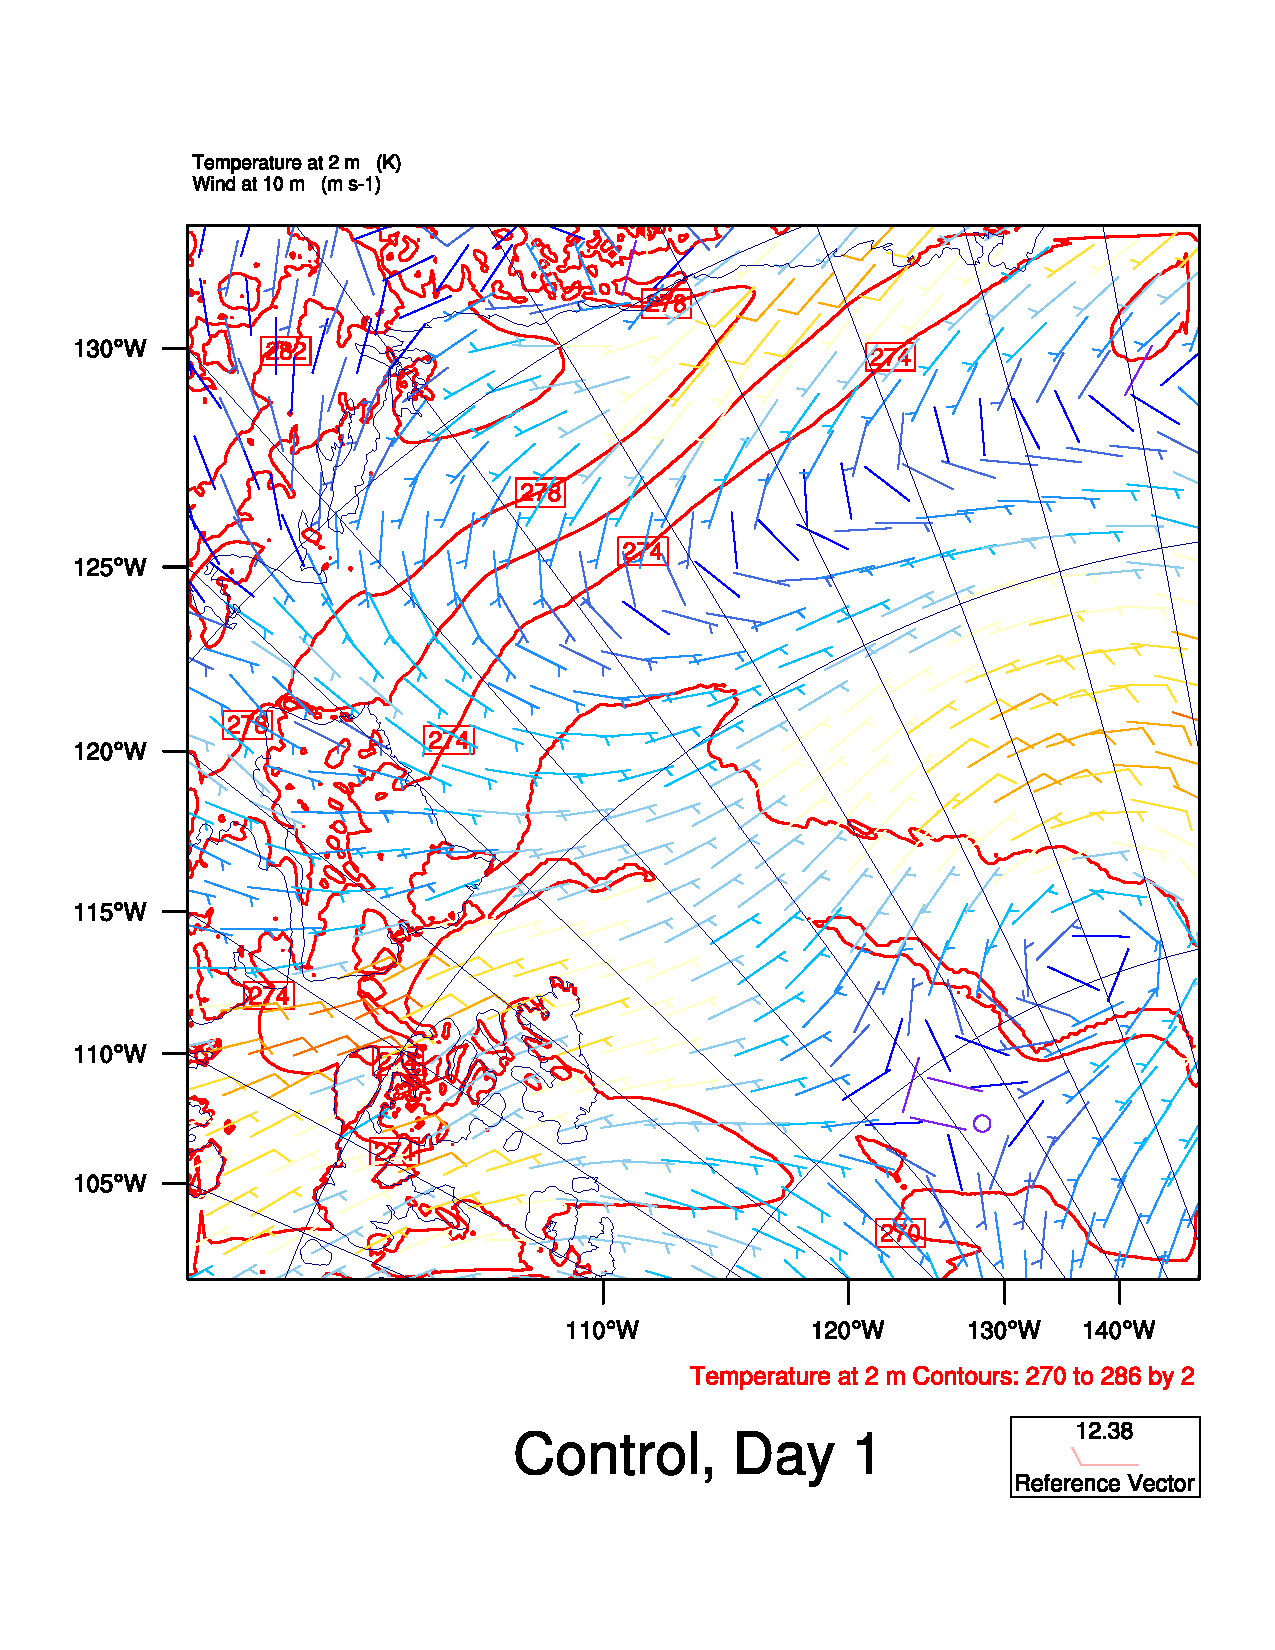
\includegraphics[width=\textwidth]{results/control/T2UV10_Control_Day1.pdf}
        \caption{Day 1}
        \label{subfig:weather_cont_day1}
    \end{subfigure}
    \begin{subfigure}{0.48\textwidth}
        \centering
        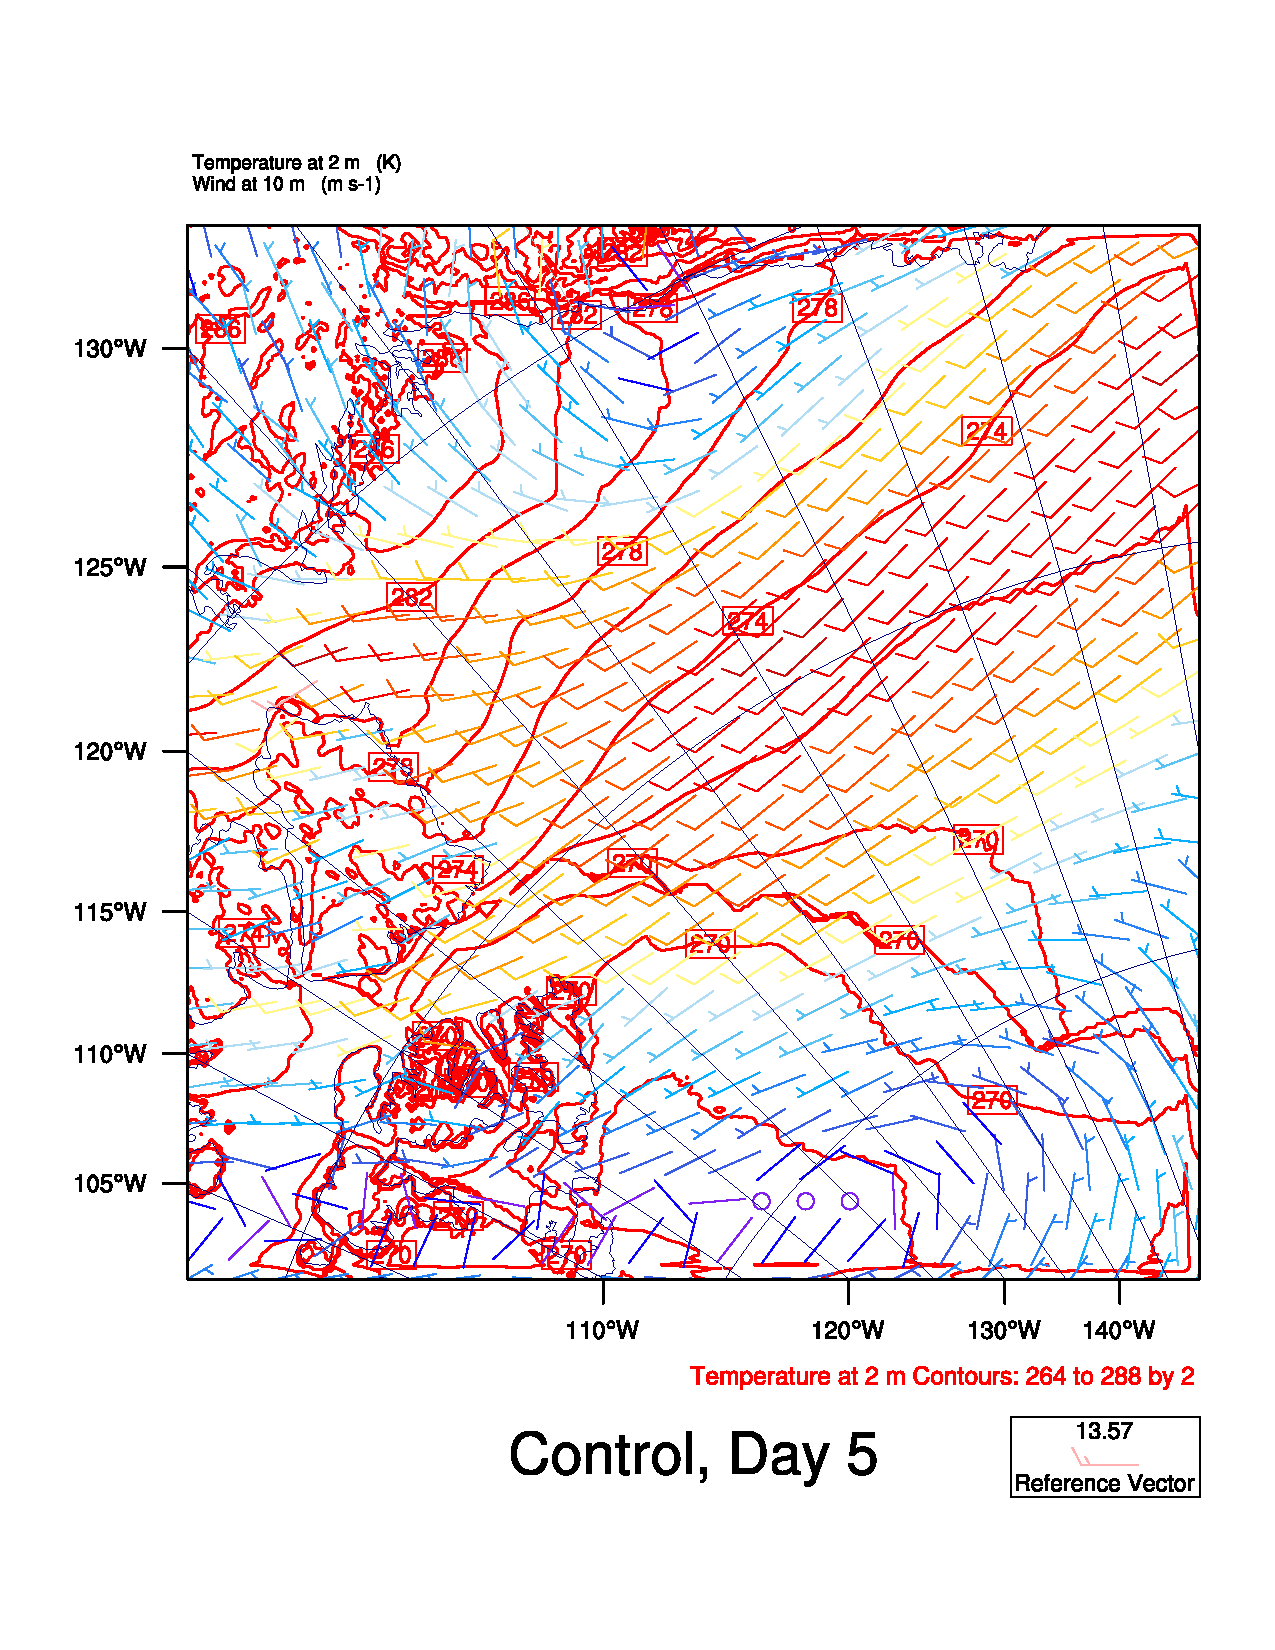
\includegraphics[width=\textwidth]{results/control/T2UV10_Control_Day5.pdf}
        \caption{Day 5}
        \label{subfig:weather_cont_day5}
    \end{subfigure}
    \caption{The temperature and wind pattern for days 1 and 5, from the control run. The temperature at 2~m height is represented by red contour lines and the wind speed and direction at 10~m height is shown by wind barbs and their color, where red indicates higher wind speed and blue indicates lower. The shortest tails on the wind barbs indicate a wind speed of 5~m/s and the longest indicate 10~m/s.}
    \label{fig:weather}
\end{figure}

By day 5 the wind direction has changed to south-easterly, see figure~\ref{subfig:weather_cont_day5}, and the clouds in the cross section, figure~\ref{subfig:cross_LWC_Day5} are low stratus over the sea ice, and there is also some thin cloud formation at the mountain, probably formed by weaker orographic lifting. There is no IWC in the section for day 5 (not shown).

\begin{figure}
    \centering
    \begin{subfigure}{0.48\textwidth}
        \centering
        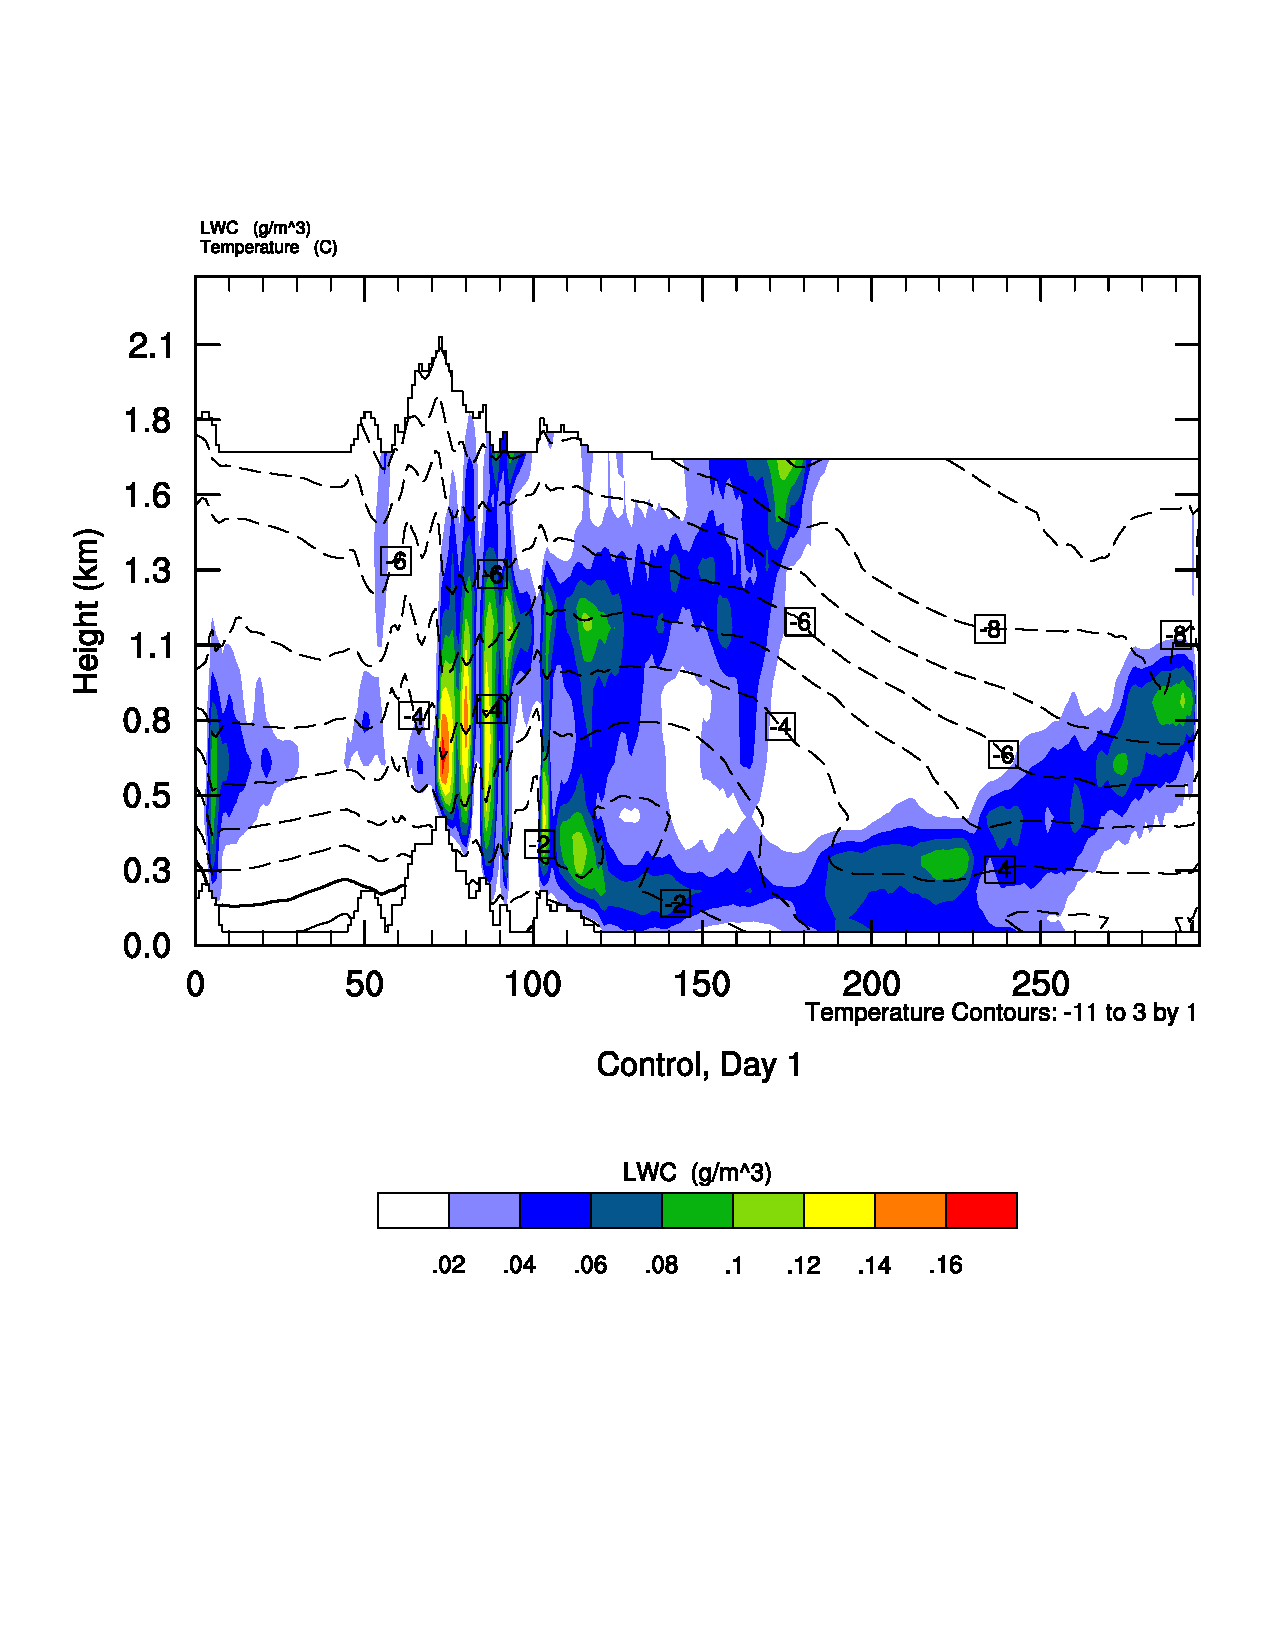
\includegraphics[width=\textwidth]{results/control/crossSec_LWC_Control_Day1.pdf}
        \caption{LWC and temperature, day 1.}
        \label{subfig:cross_LWC_day1}
    \end{subfigure}
    \begin{subfigure}{0.48\textwidth}
        \centering
        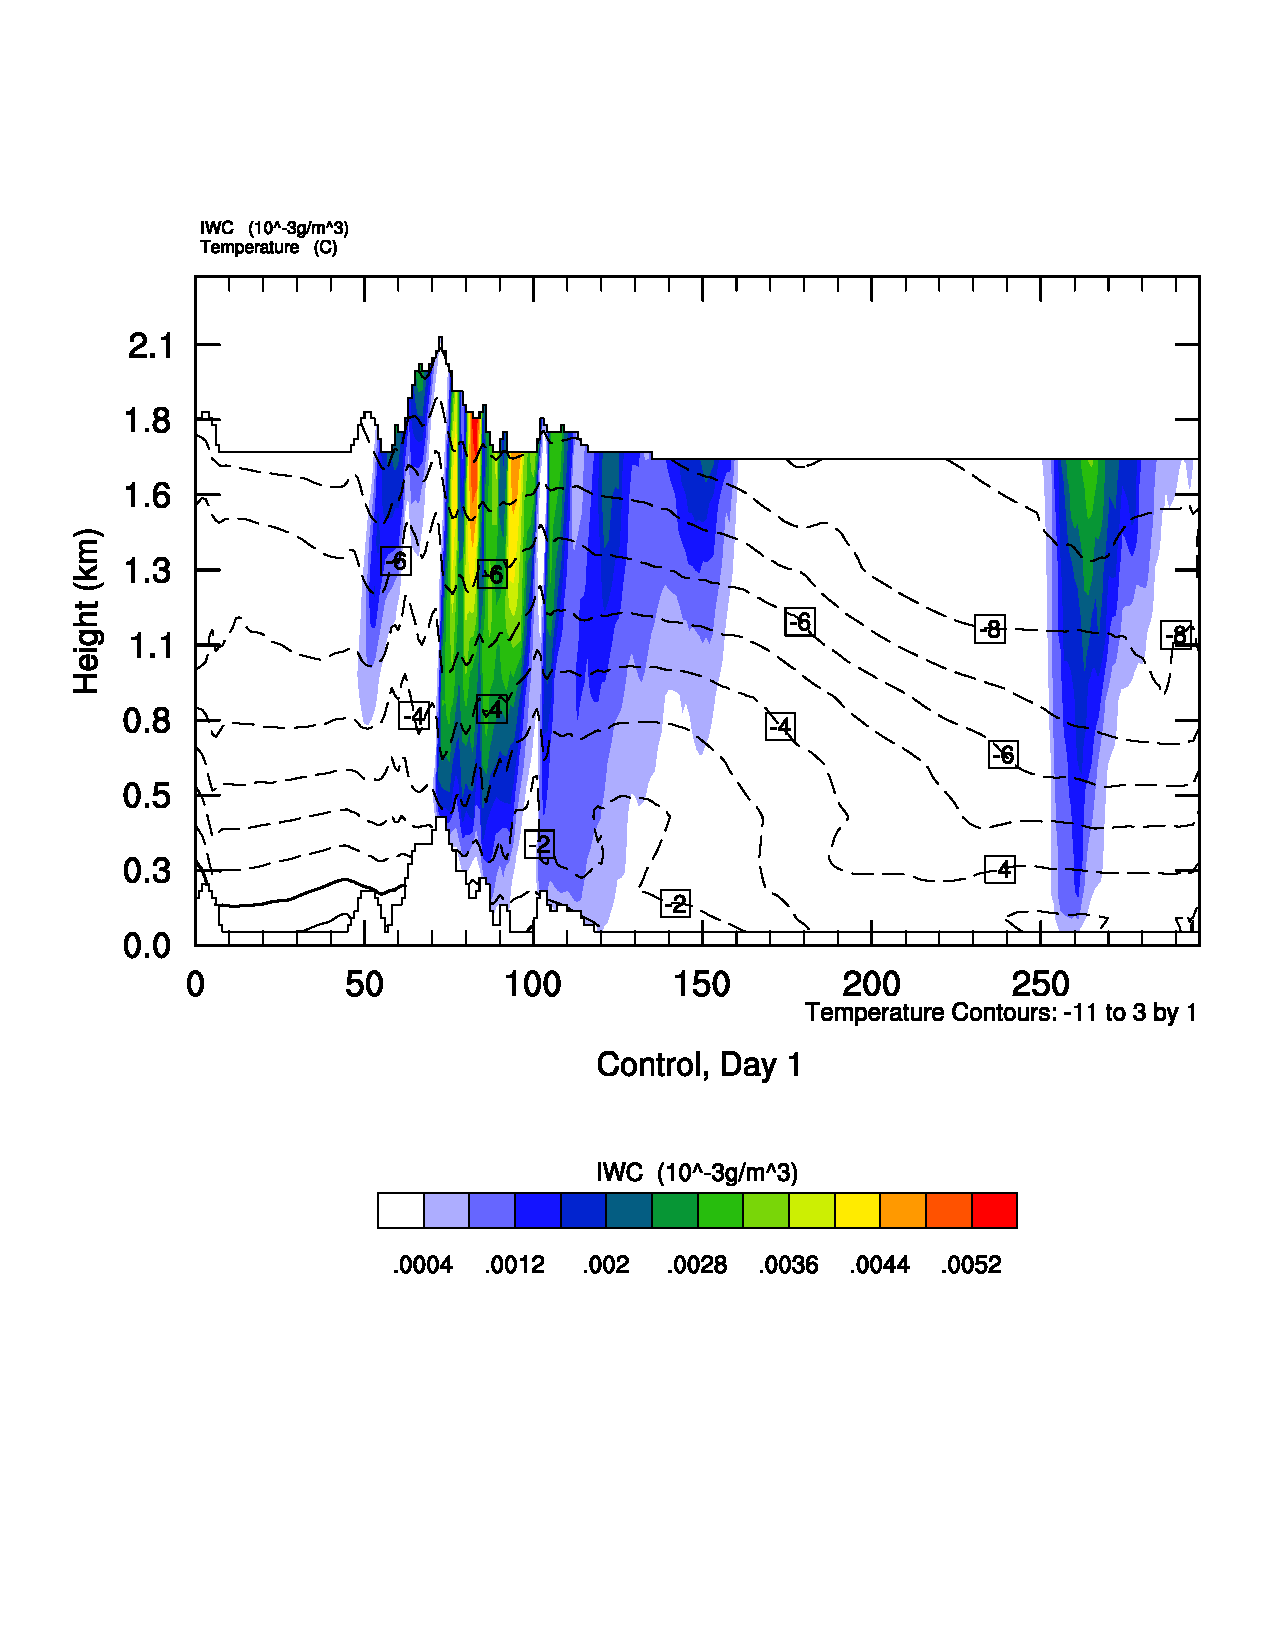
\includegraphics[width=\textwidth]{results/control/crossSec_IWC_Control_Day1.pdf}
        \caption{IWC and temperature, day1.}
        \label{subfig:cross_IWC_day1}
    \end{subfigure}
    
    \begin{subfigure}{0.48\textwidth}
        \centering
        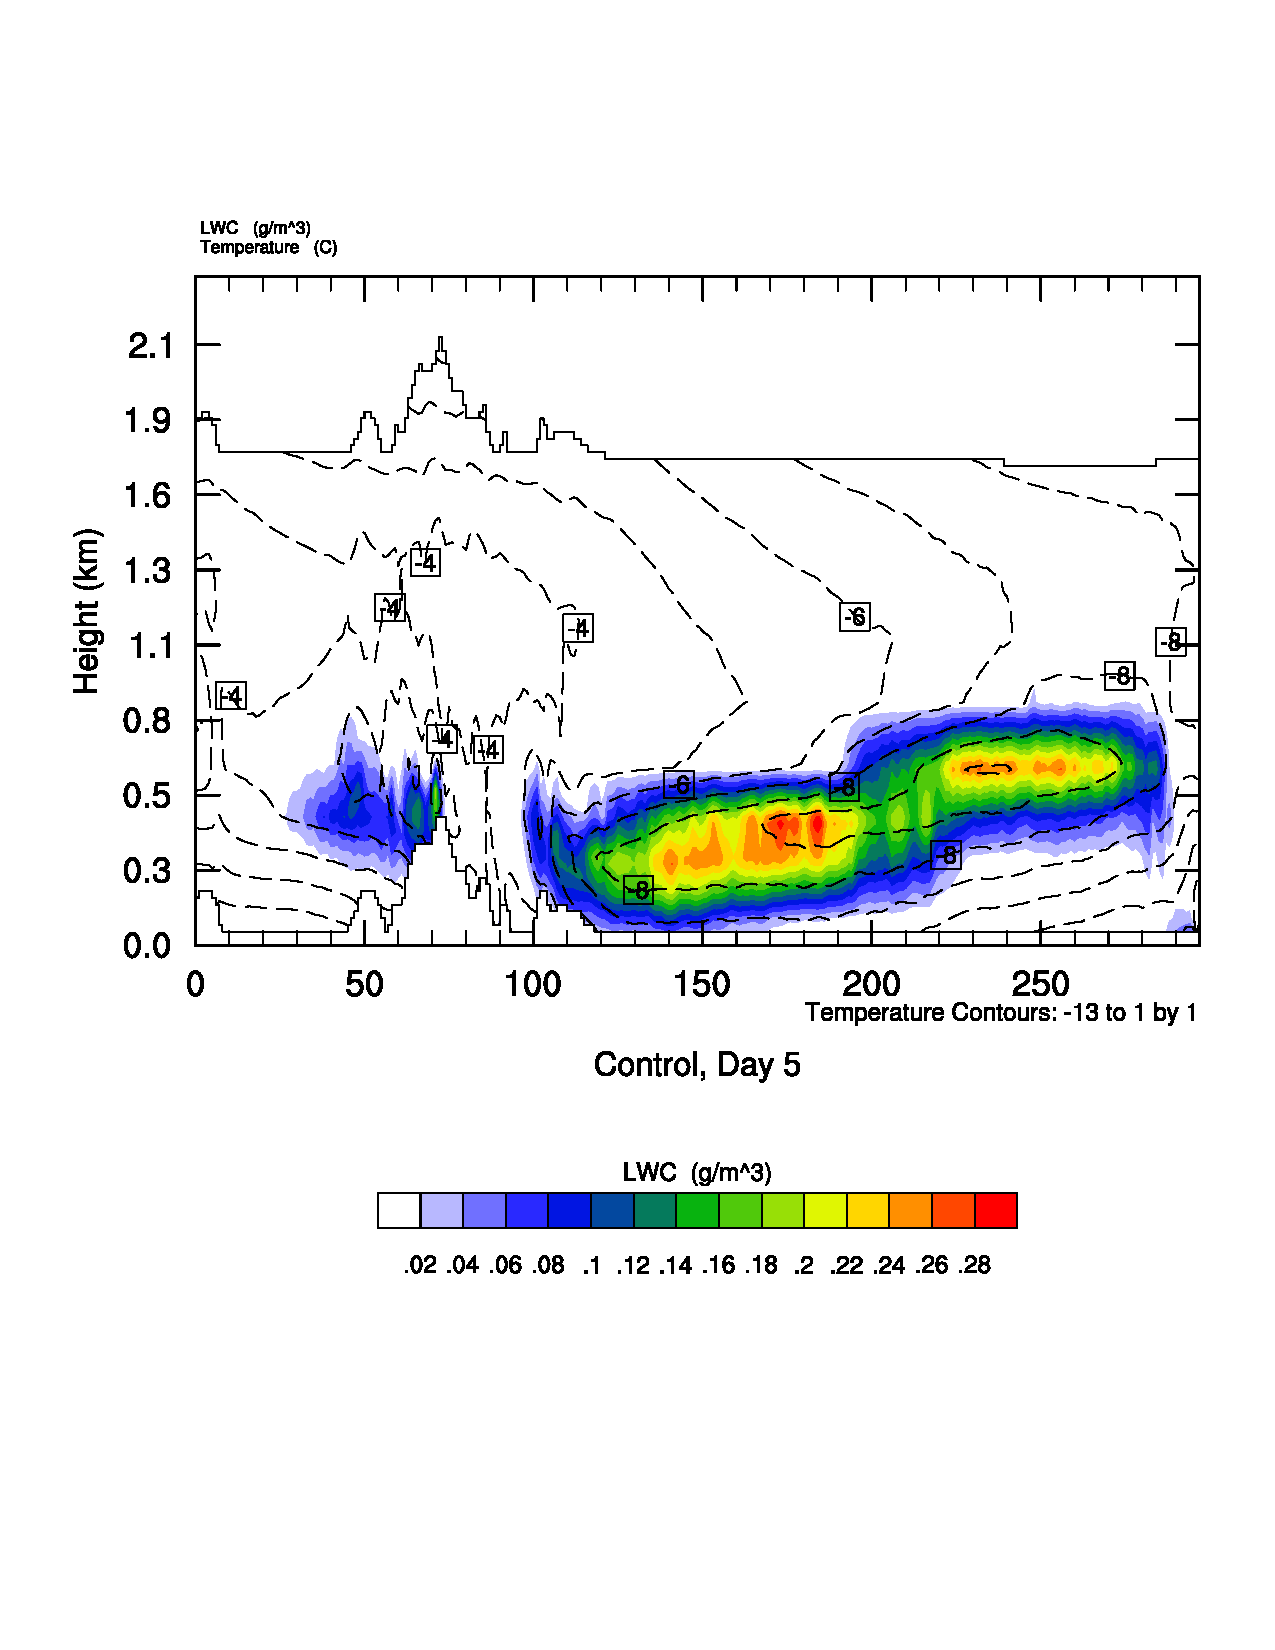
\includegraphics[width=\textwidth]{results/control/crossSec_LWC_Control_Day5.pdf}
        \caption{LWC and temperature, day 5.}
        \label{subfig:cross_LWC_Day5}
    \end{subfigure}
    \begin{subfigure}{0.48\textwidth}
        \centering
        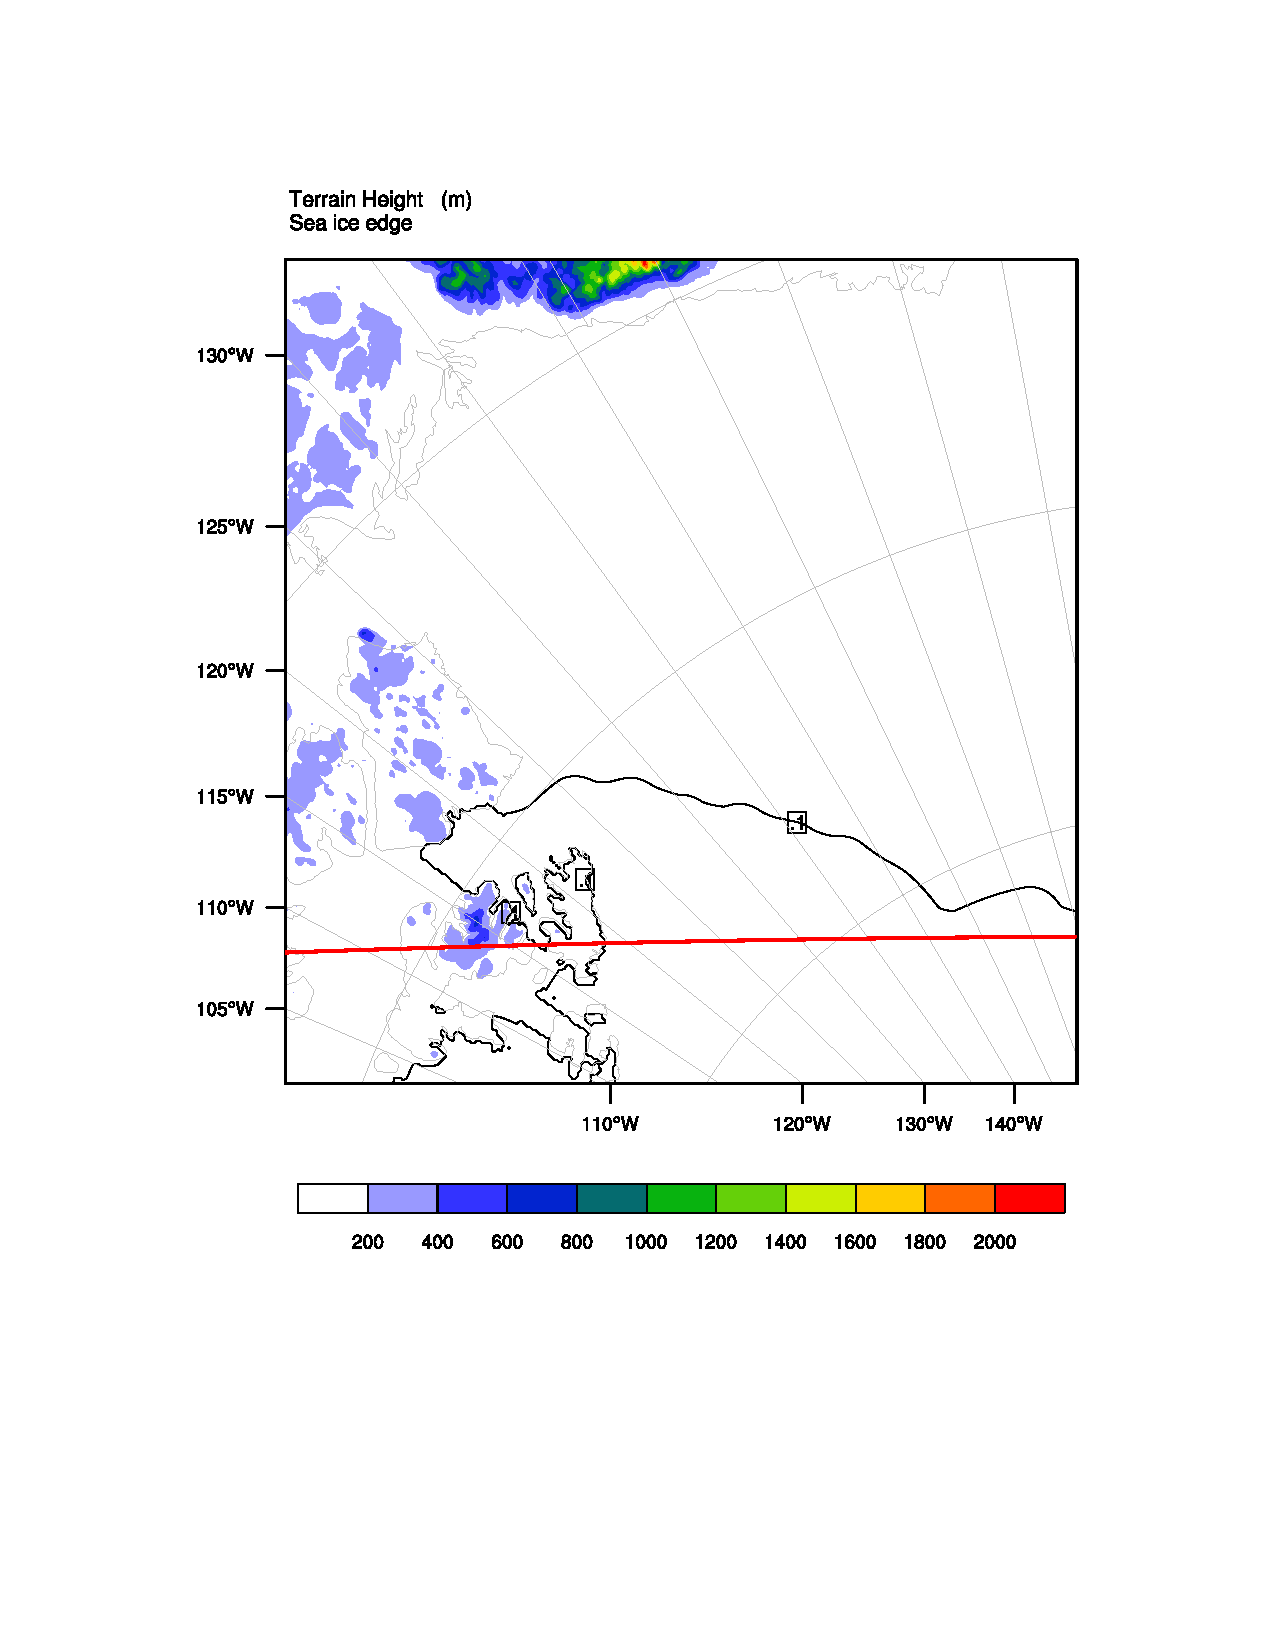
\includegraphics[width=\textwidth]{results/control/crossSec_line.pdf}
        \caption{Line over which the vertical cross sections are made.}
        \label{subfig:cross_line}
    \end{subfigure}
    \caption{Vertical cross sections of averaged liquid ($\text{g/m}^3$) and ice  ($\text{mg/m}^3$) water content, as filled contours, with temperature ($\degree\text{C}$) as dashed contours, from the control run, for days 1 and 5. LWC and IWC for day 1 are shown in figures~\ref{subfig:cross_LWC_day1} and~\ref{subfig:cross_IWC_day1} respectively. Figure~\ref{subfig:cross_LWC_Day5} shows the LWC for day 5. The IWC on day 5 was 0 in the section and is not shown. Figure~\ref{subfig:cross_line} shows a map of the area with the ice edge as a black contour line. The terrain height is represented by filled contours and the red line over the sea ice is the line over which the cross sections are made.}
    \label{fig:sections}
\end{figure}

The LWP for days 1 and 5 are shown in figure~\ref{subfig:LWPr1Day1} and~\ref{subfig:LWPr1Day5} with the CDNC~(\ref{subfig:cdnc_cont_Day1} and~\ref{subfig:cdnc_cont_Day5}) and $r_e$~(\ref{subfig:recloud_r1Day1} and~\ref{subfig:recloud_r1Day5}). One can clearly see that the LWP and the CDNC have similar pattern, which is expected based on equation~\ref{eqn:LWC}. The pattern in $r_e$ also fits quite well with that of LWP, meaning that larger droplets contain more water.

%---------- LWP control run, days 1 and 5
\begin{figure}
    \centering
    \begin{subfigure}{0.40\textwidth}
        \centering
        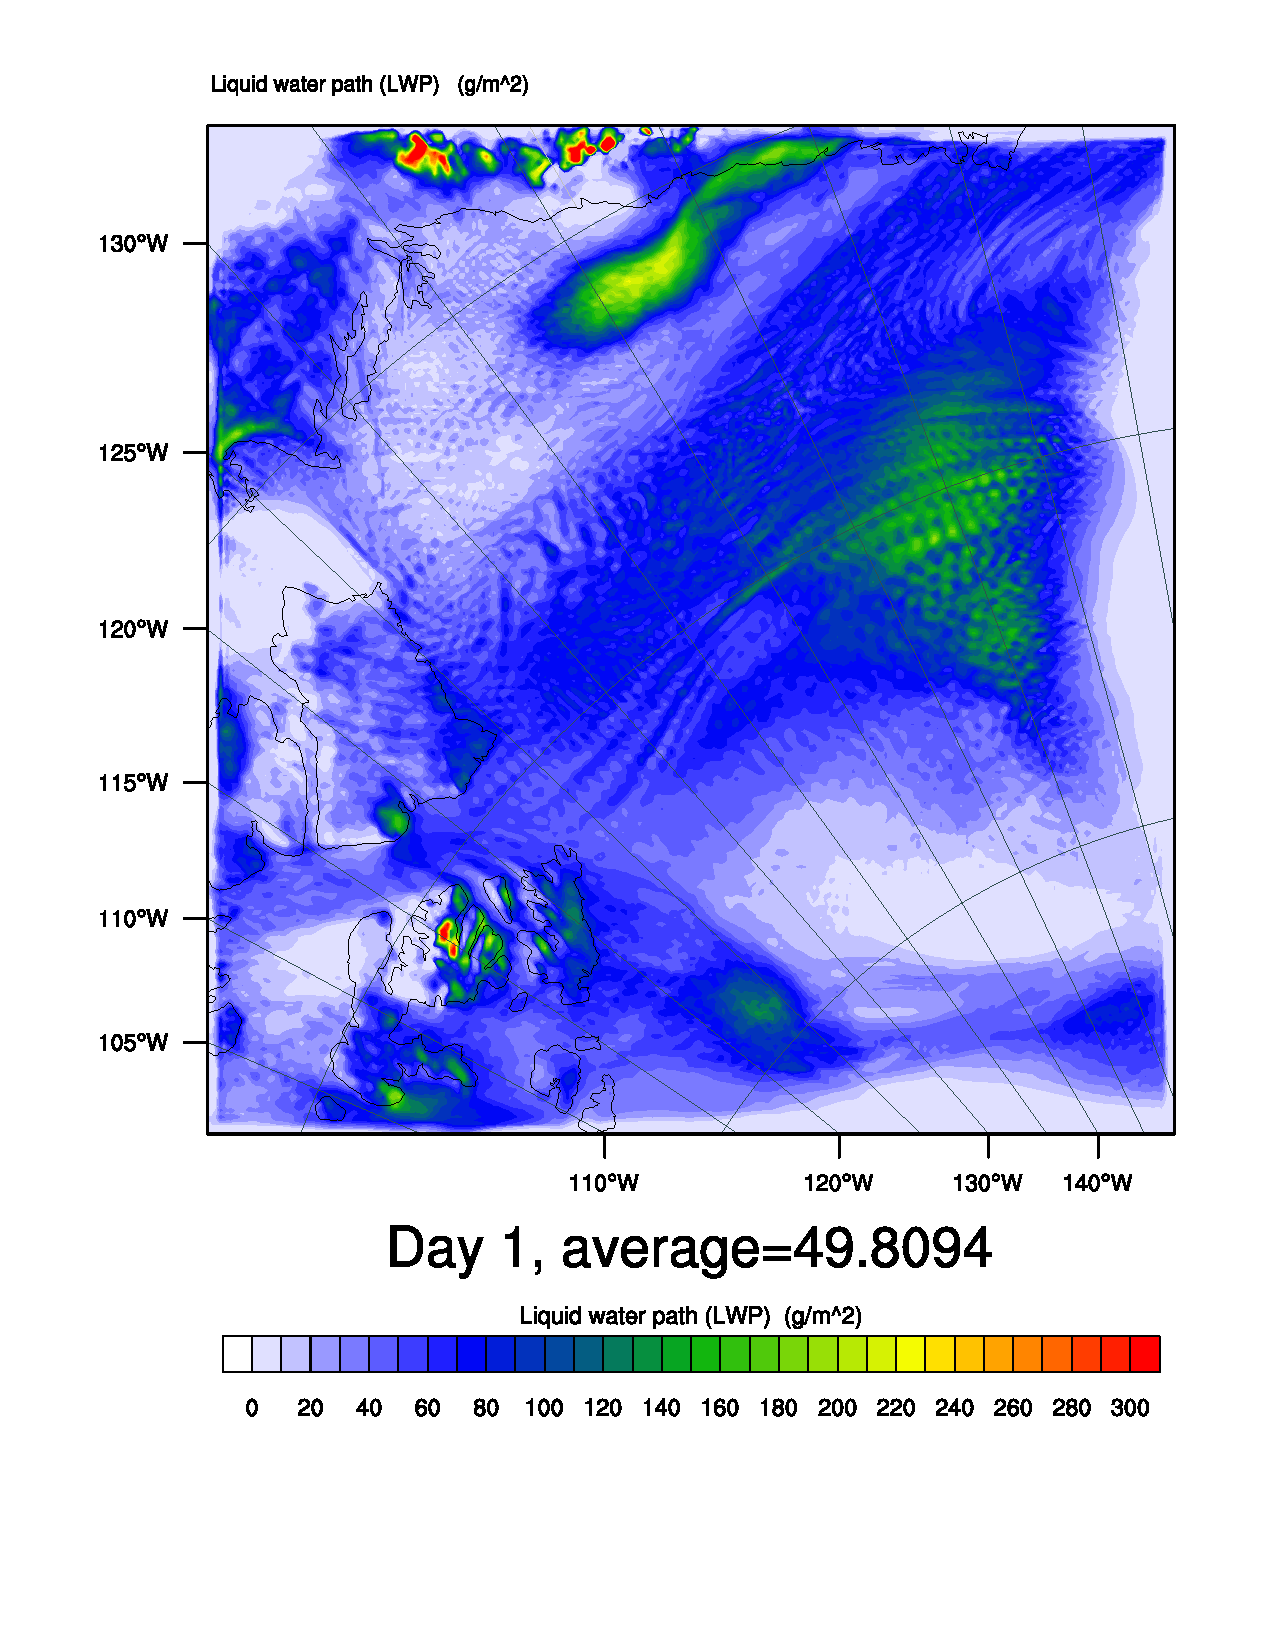
\includegraphics[width=\textwidth]{results/control/LWP_Day1.pdf}
        \caption{LWP day 1.}
        \label{subfig:LWPr1Day1}
    \end{subfigure}
    \begin{subfigure}{0.40\textwidth}
        \centering
        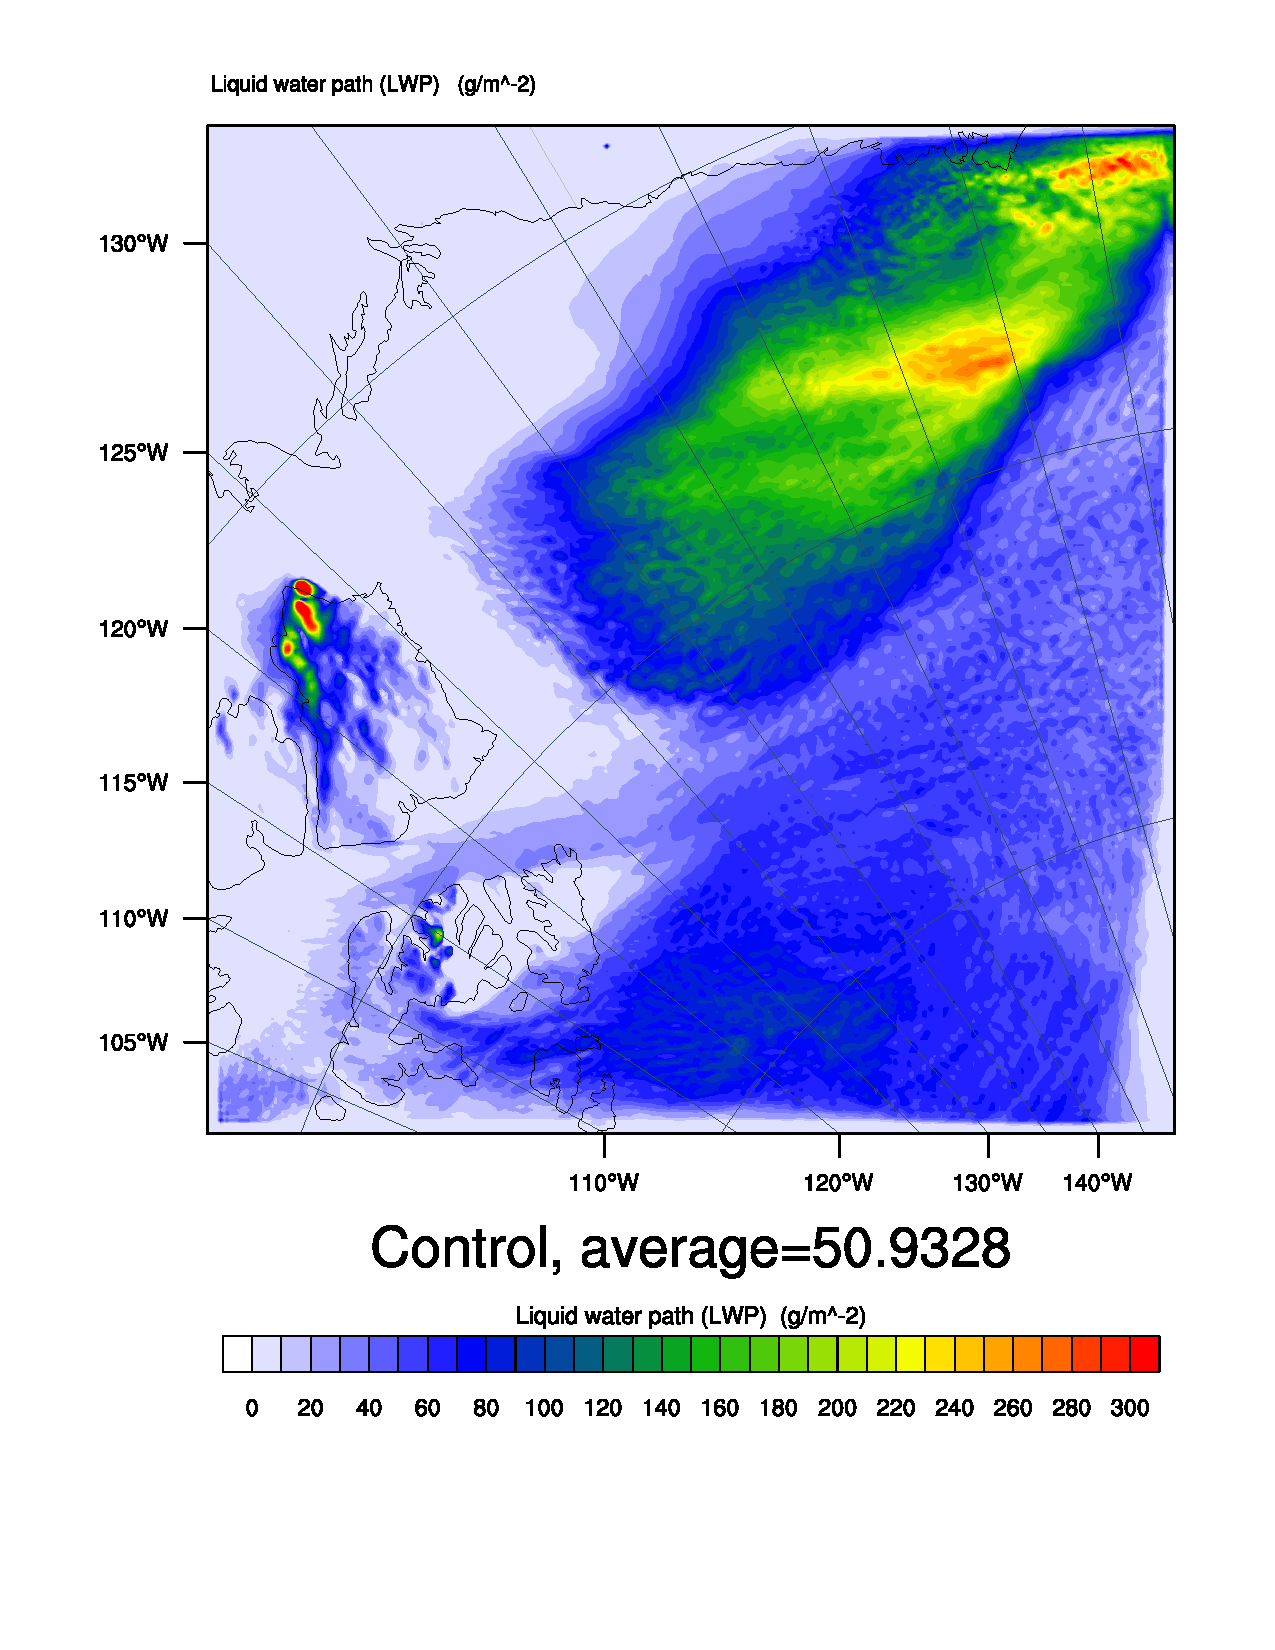
\includegraphics[width=\textwidth]{results/control/LWP_Day5.pdf}
        \caption{LWP day 5.}
        \label{subfig:LWPr1Day5}
    \end{subfigure}

%------CDNC
	\begin{subfigure}{0.40\textwidth}
		\centering
		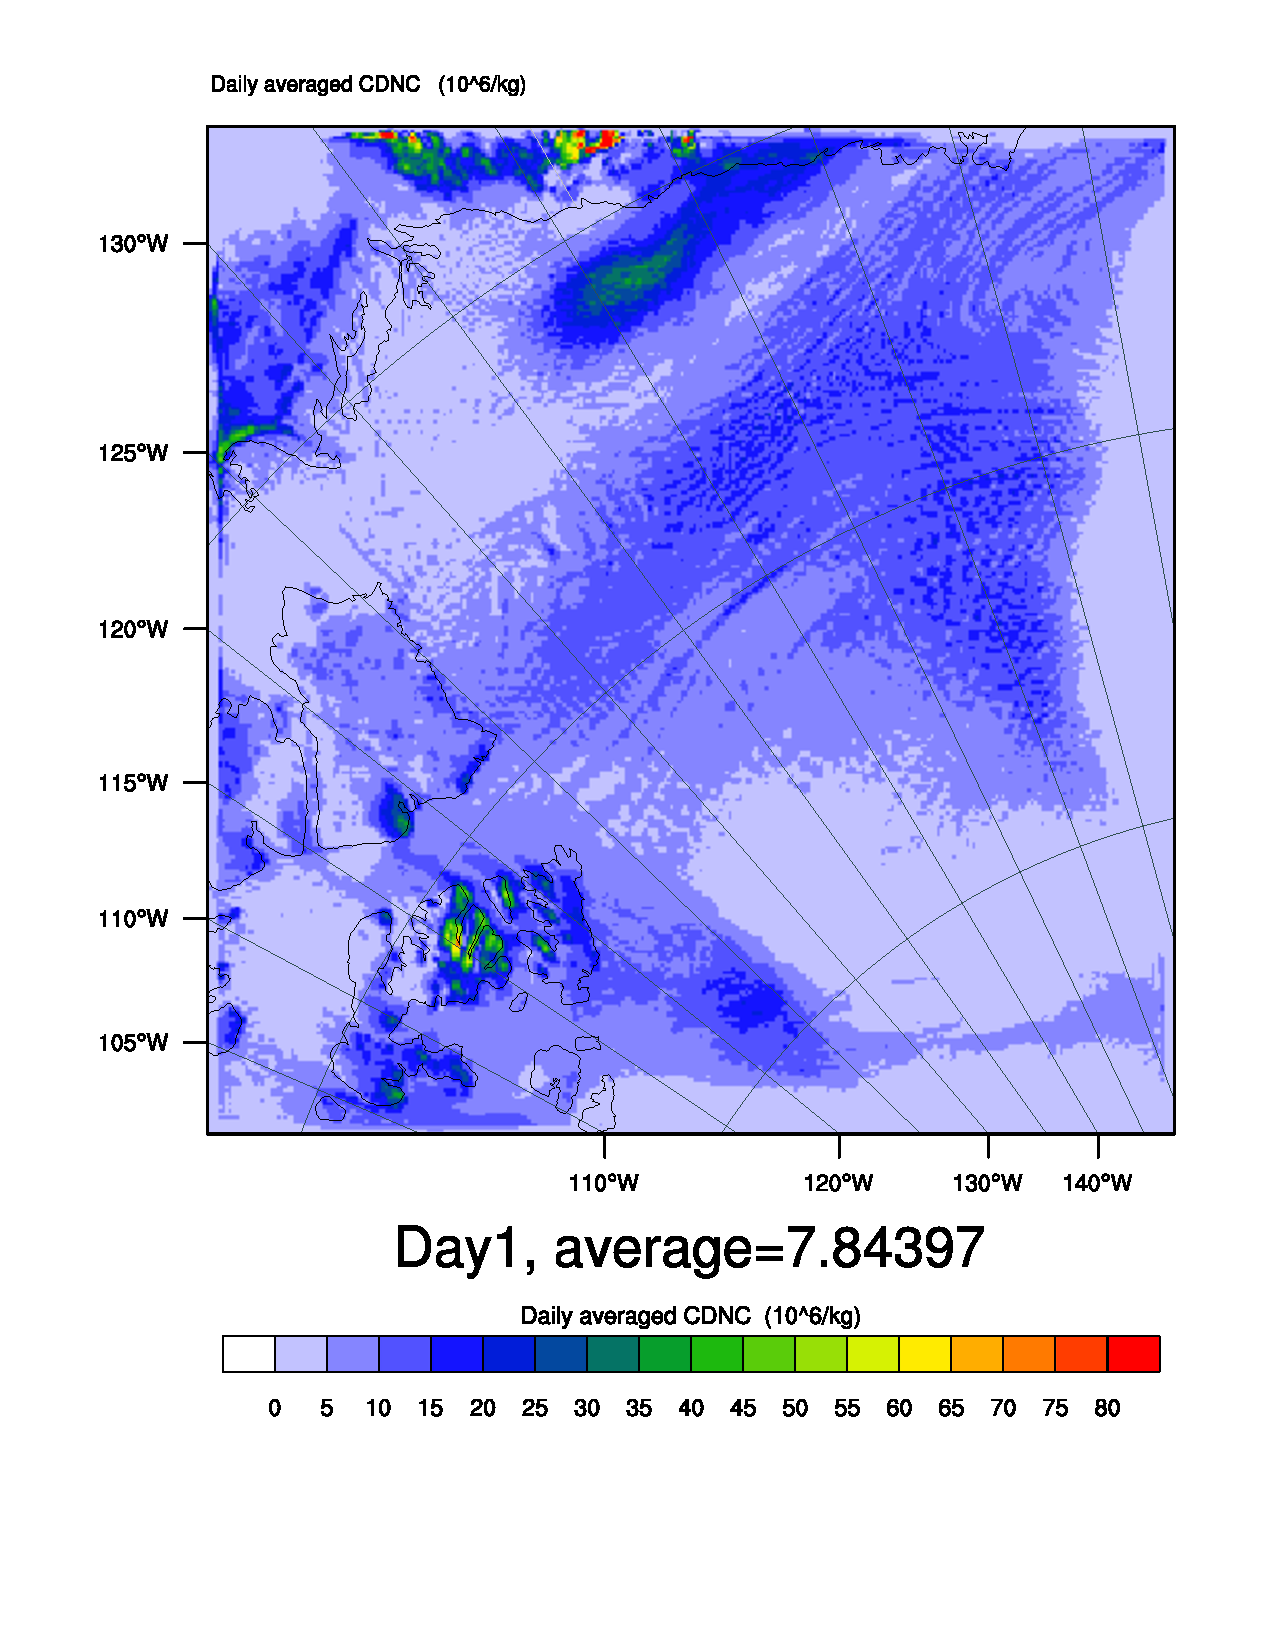
\includegraphics[width=\textwidth]{results/control/QNCLOUD_Day1.pdf}
		\caption{CDNC day 1.}
		\label{subfig:cdnc_cont_Day1}
	\end{subfigure}
	\begin{subfigure}{0.40\textwidth}
		\centering
		\includegraphics[width=\textwidth]{results/control/QNCLOUD_day5.pdf}
		\caption{CDNC day 5.}
		\label{subfig:cdnc_cont_Day5}
	\end{subfigure}
	
%----------- Effective radius, days 1 and 5
	\begin{subfigure}{0.40\textwidth}
		\centering
		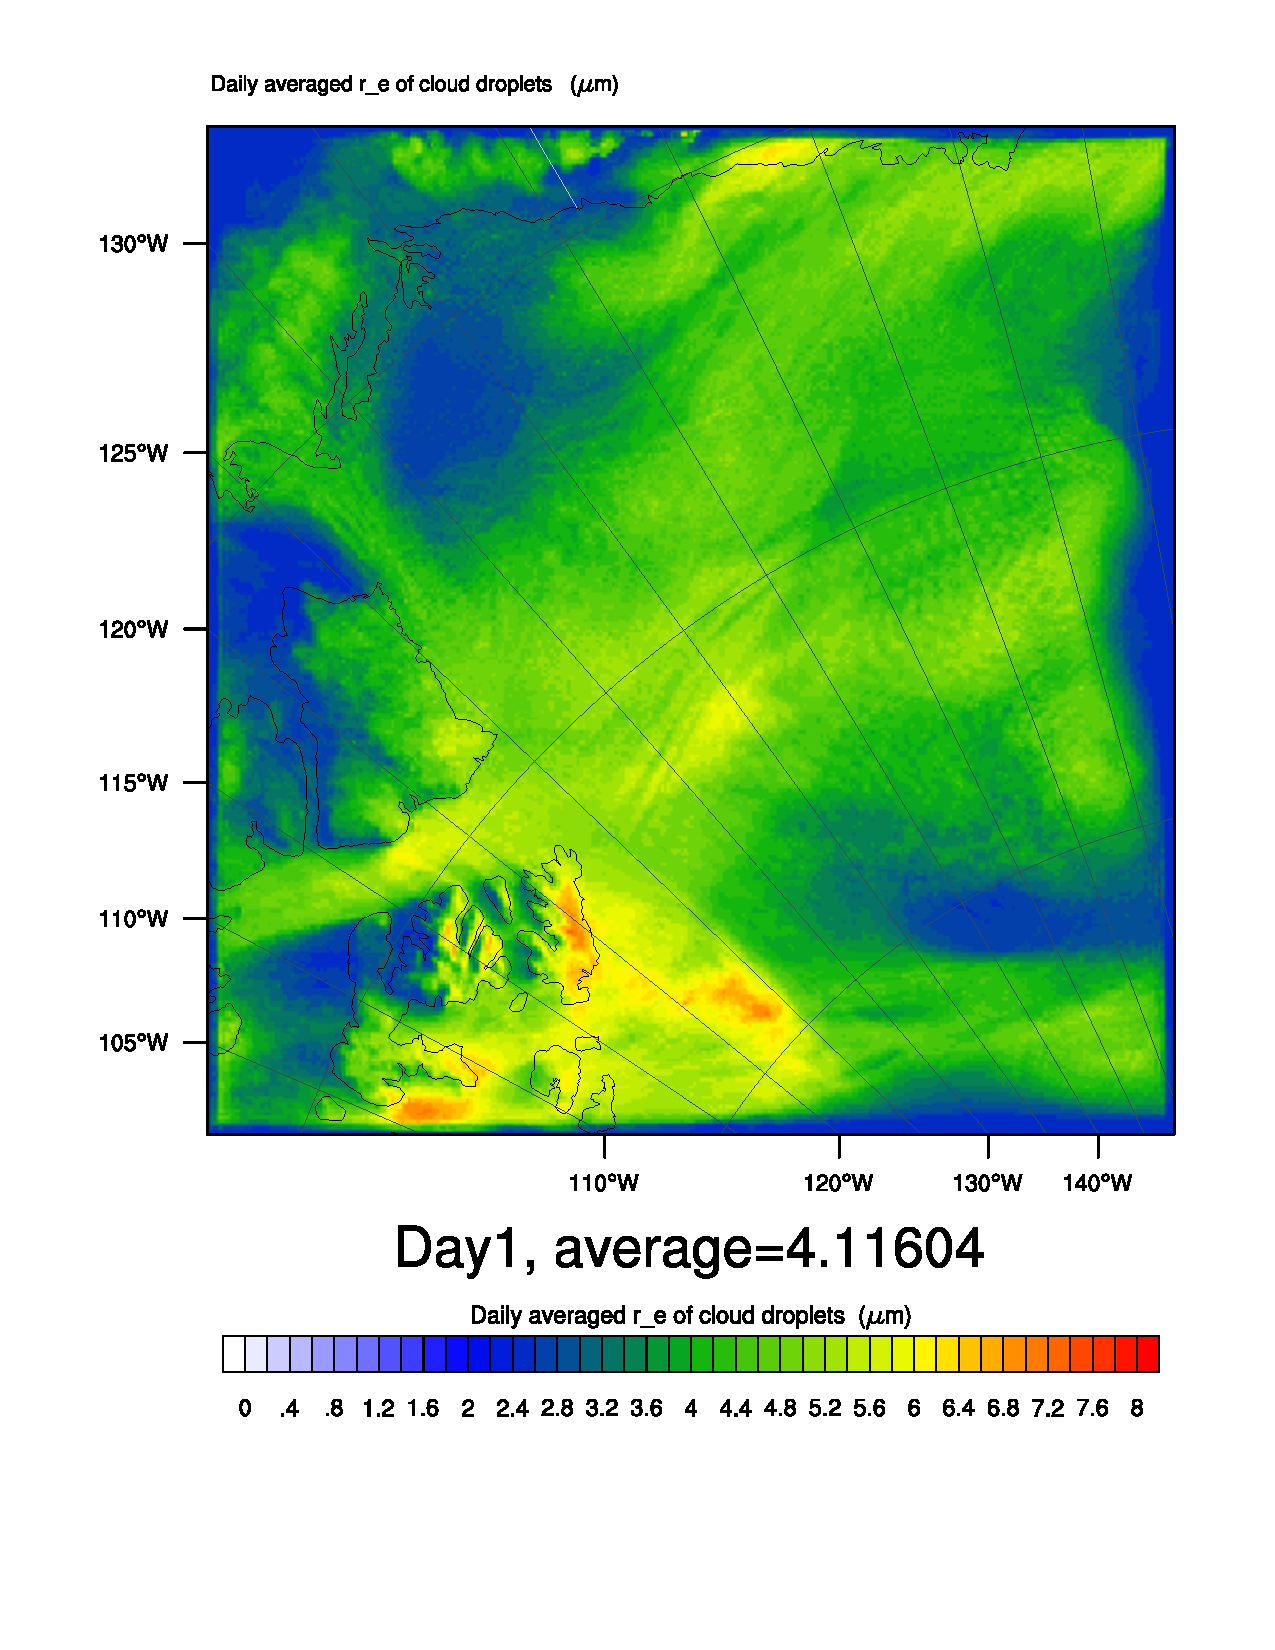
\includegraphics[width=\textwidth]{results/control/RE_CLOUD_Day1.pdf}
		\caption{$r_e$ day1.}
		\label{subfig:recloud_r1Day1}
	\end{subfigure}
	\begin{subfigure}{0.40\textwidth}
		\centering
		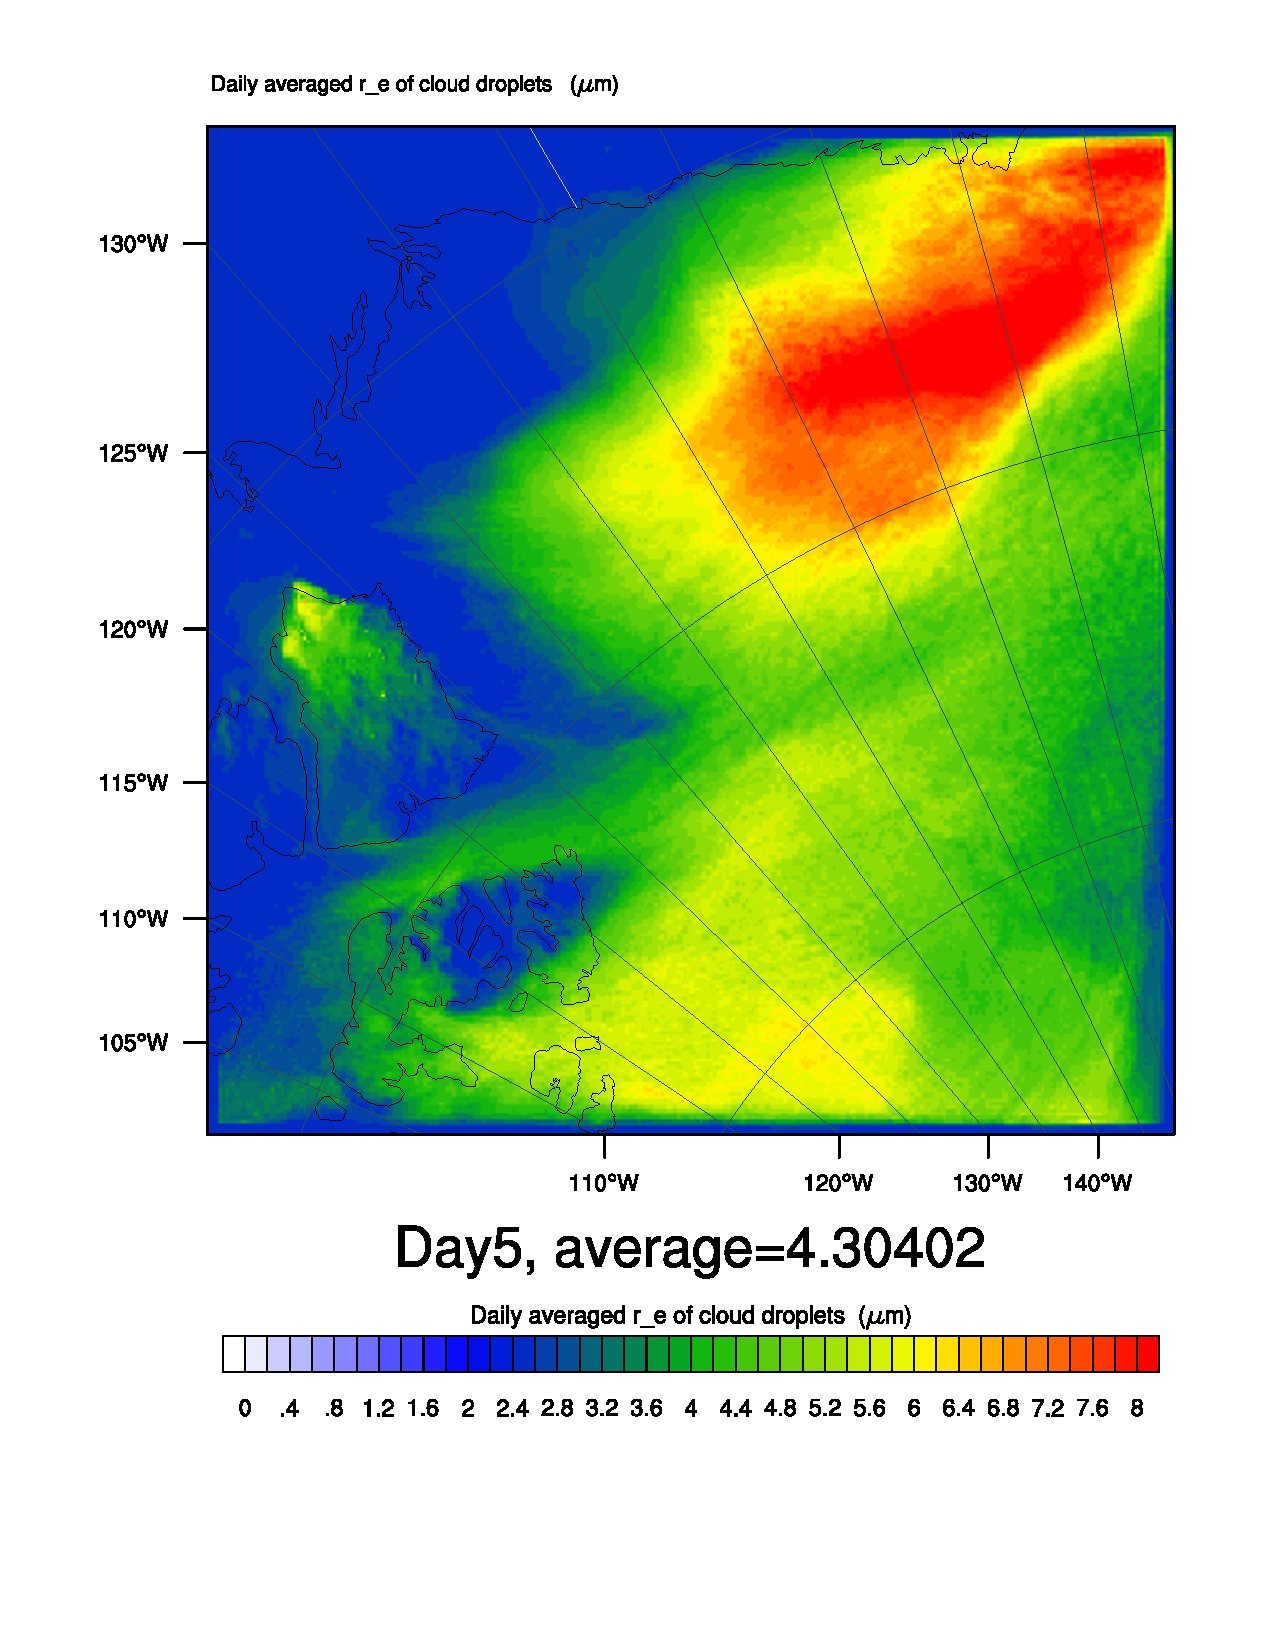
\includegraphics[width=\textwidth]{results/control/RE_CLOUD_Day5.pdf}
		\caption{$r_e$ day 5.}
		\label{subfig:recloud_r1Day5}
	\end{subfigure}
	\caption{LWP averaged in time, and CDNC and $r_e$ averaged over the lowermost 11 layers and time, for days 1 and 5. Control.}
	\label{fig:recloud_r1}
\end{figure}


The fluxes of both SW and LW radiation at both downward at the surface and upward at the top of the atmosphere (TOA) may be partly explained by the clouds (@utdyp, Jon egill spør: Hvordan det?), through looking at the LWP. Figures~\ref{fig:radiation_r1Day1} and~\ref{fig:radiation_r1Day5} show the downward SW and LW at the surface and upward at TOA for days 1 and 5 respectively.
%----------Radiation Day 1
\begin{figure}
\centering
	\begin{subfigure}{0.48\textwidth}
		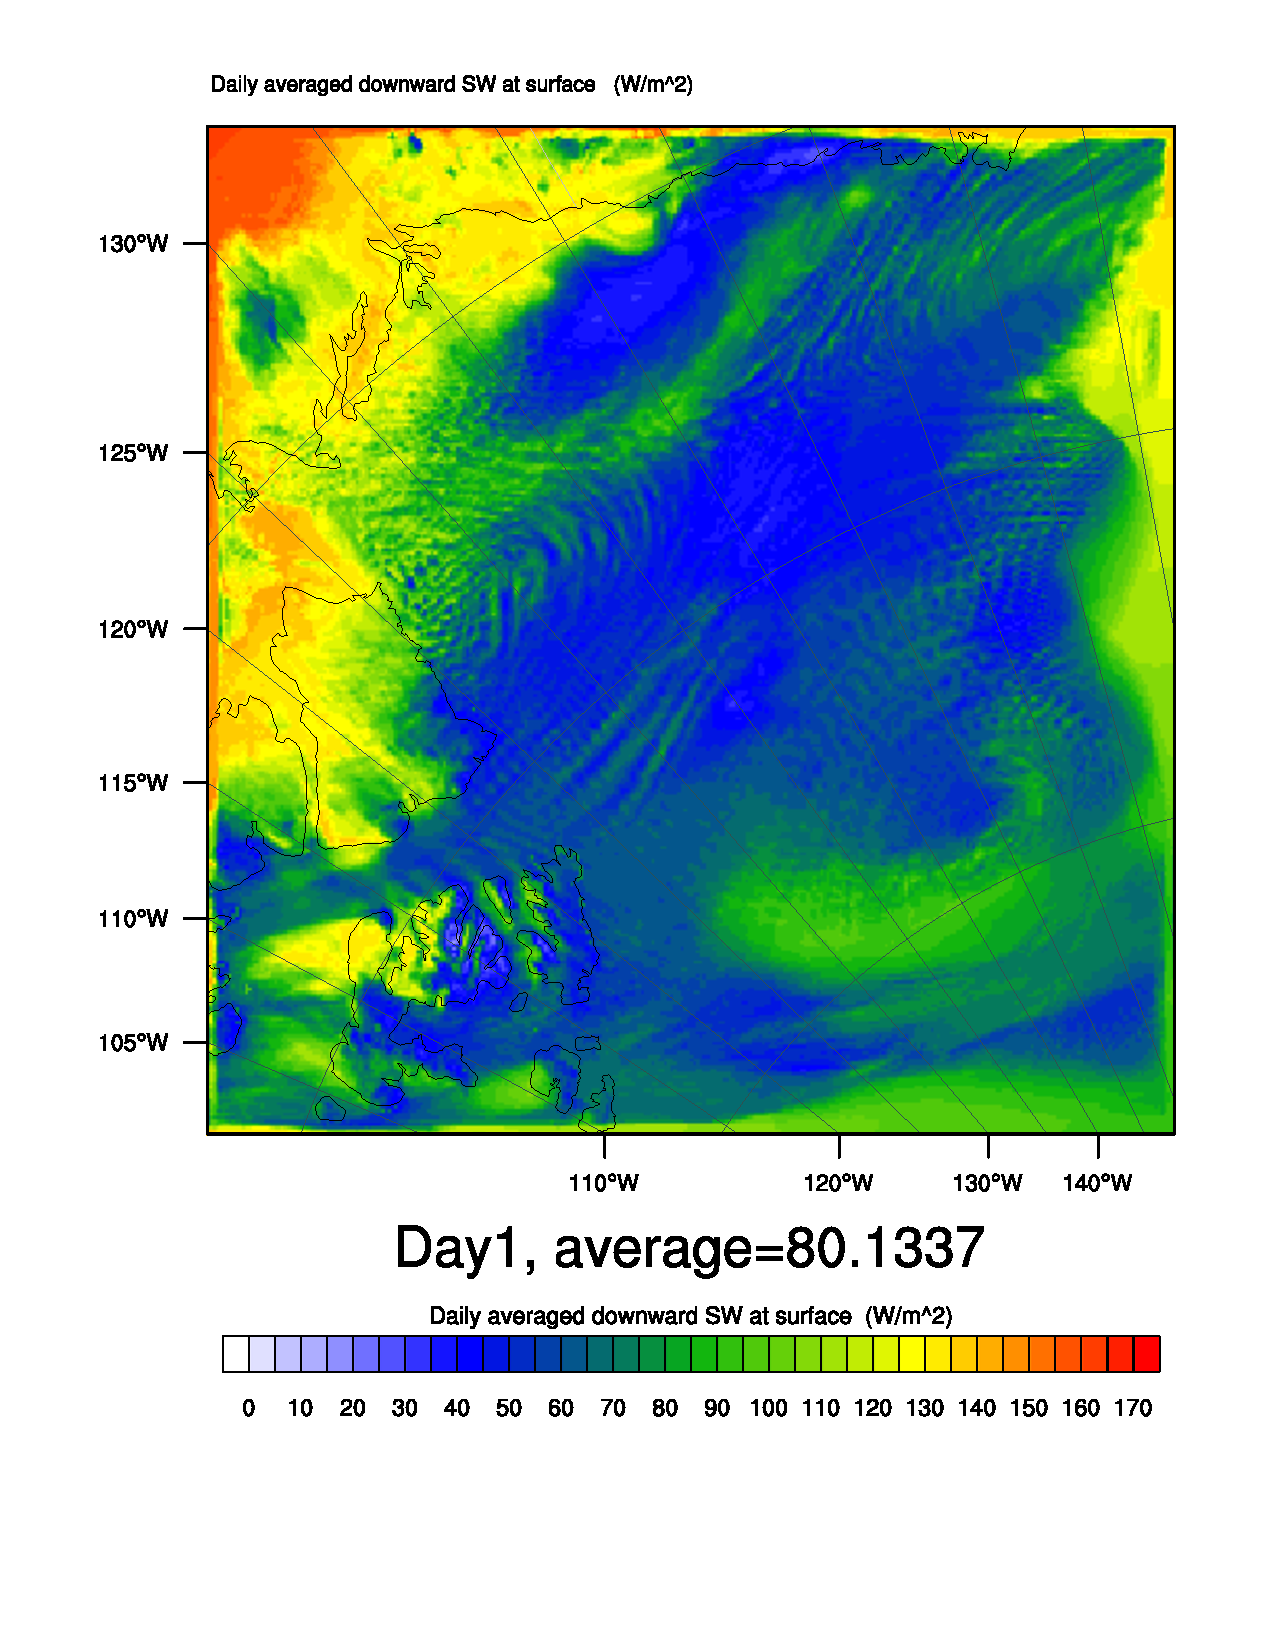
\includegraphics[width=\textwidth]{results/control/SWDOWN_Day1.pdf}
		\caption{SW down at the surface, day 1.}
		\label{subfig:swdown_r1Day1}
	\end{subfigure}
	\quad
	\begin{subfigure}{0.48\textwidth}
		\centering
		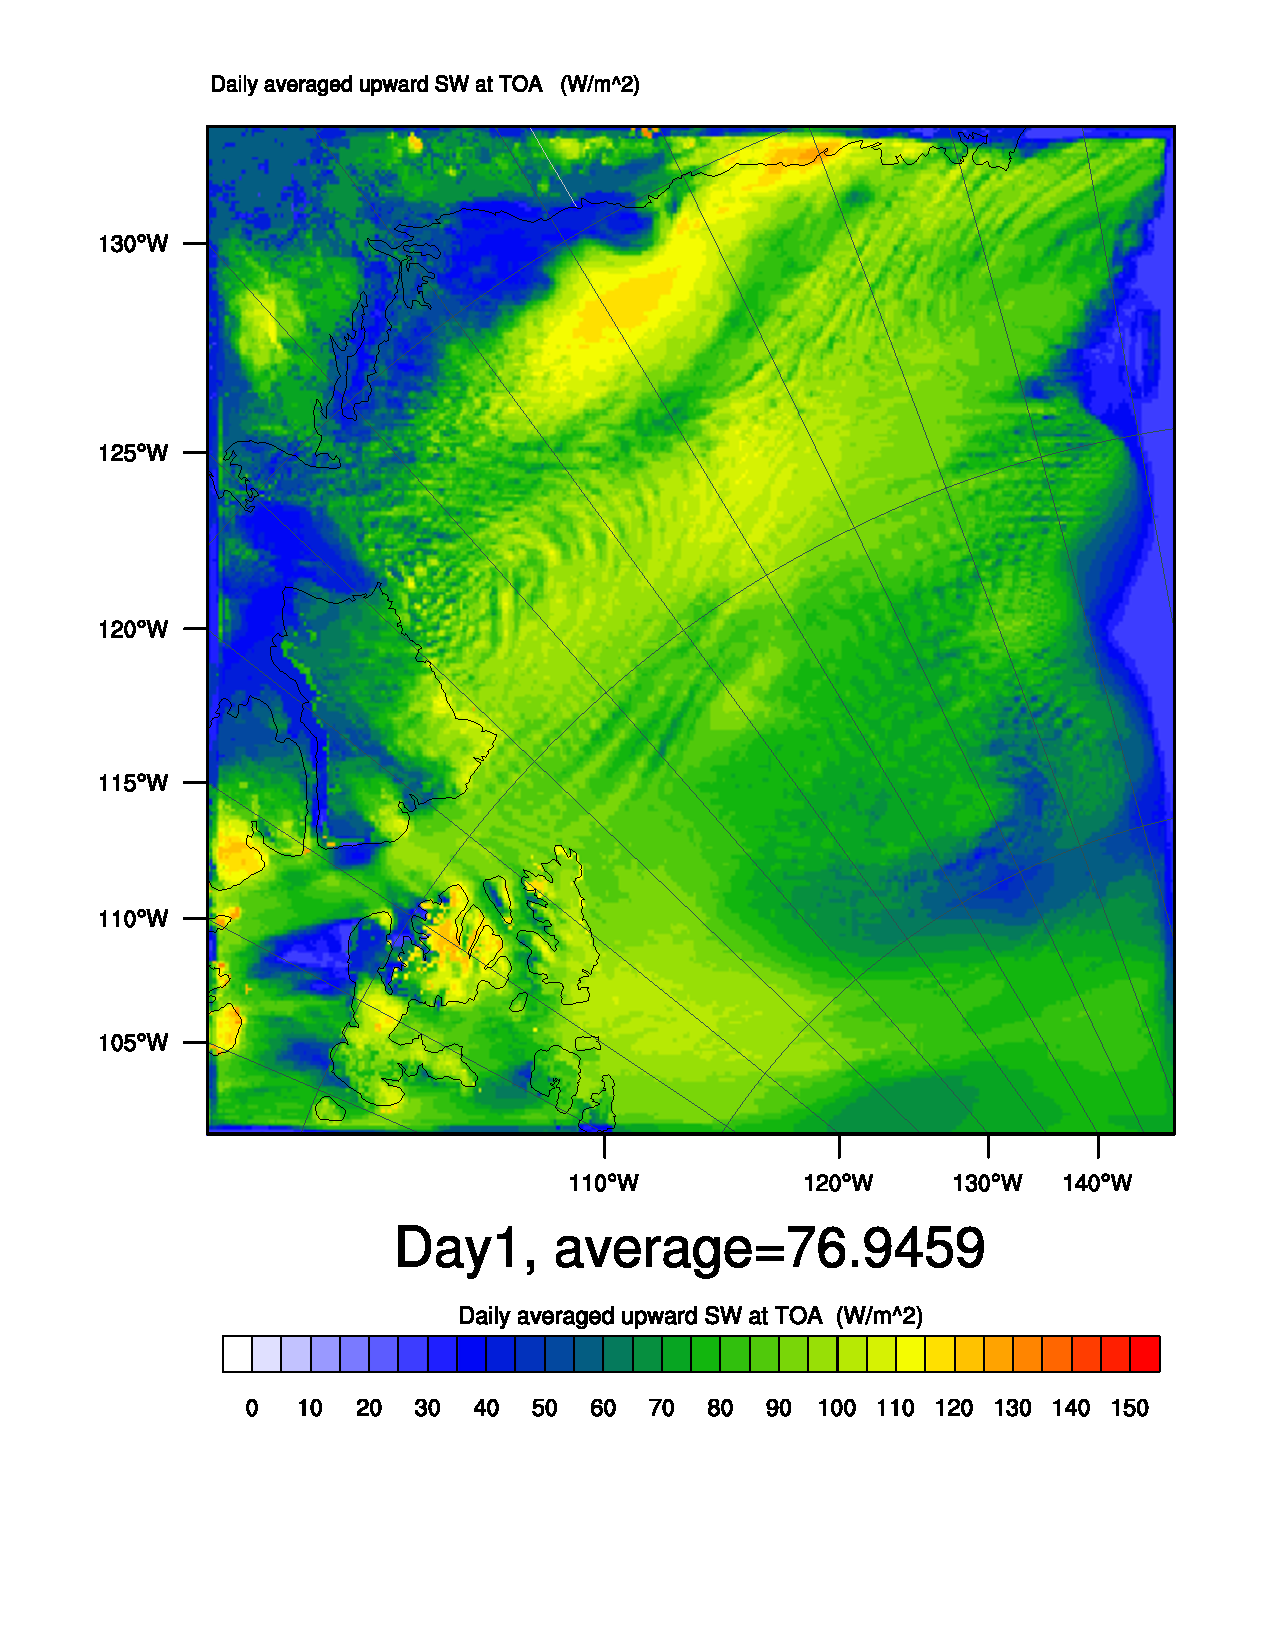
\includegraphics[width=\textwidth]{results/control/SWUPT_Day1.pdf}
		\caption{SW up at TOA, day 1.}
		\label{subfig:swup_r1Day1}
	\end{subfigure}
	
	\begin{subfigure}{0.48\textwidth}
		\centering
		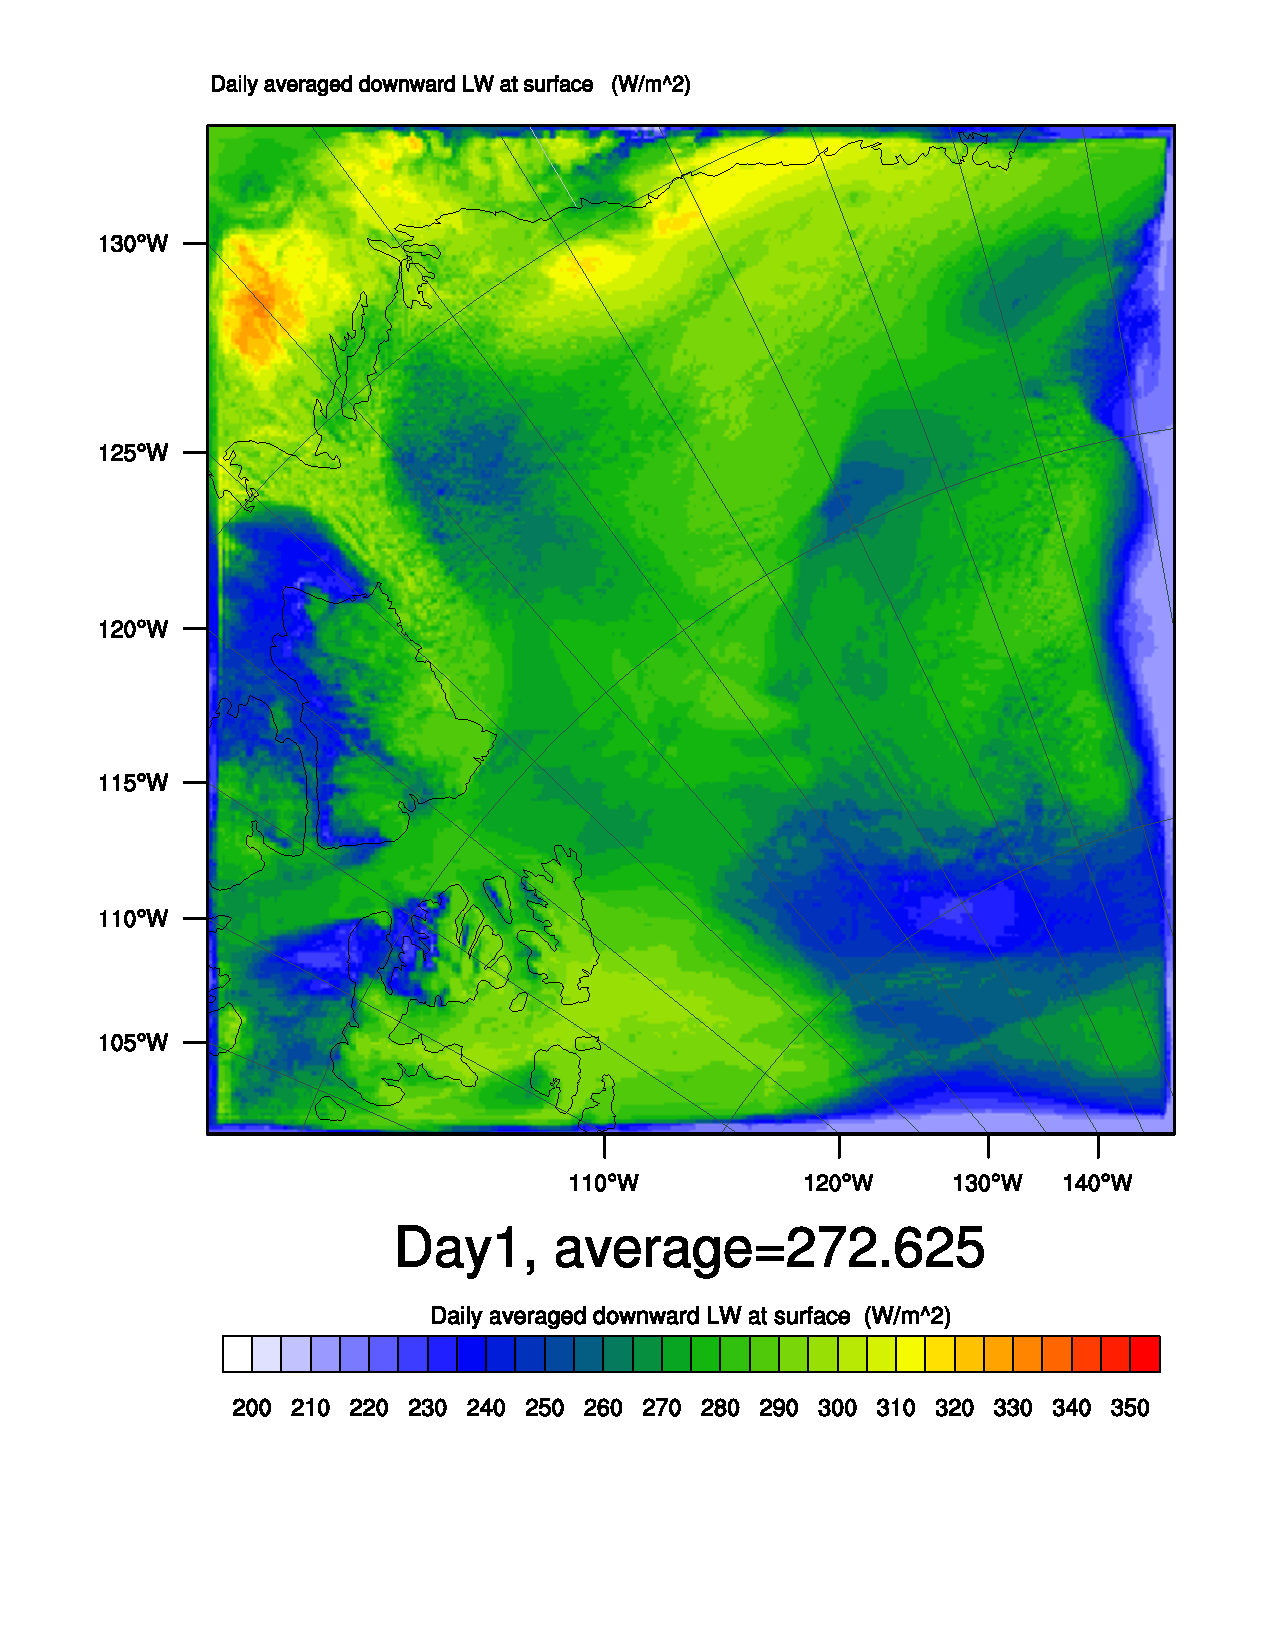
\includegraphics[width=\textwidth]{results/control/GLW_Day1.pdf}
		\caption{LW down at the surface, day 1.}
		\label{subfig:glw_r1Day1}
	\end{subfigure}
	\quad
	\begin{subfigure}{0.48\textwidth}
		\centering
		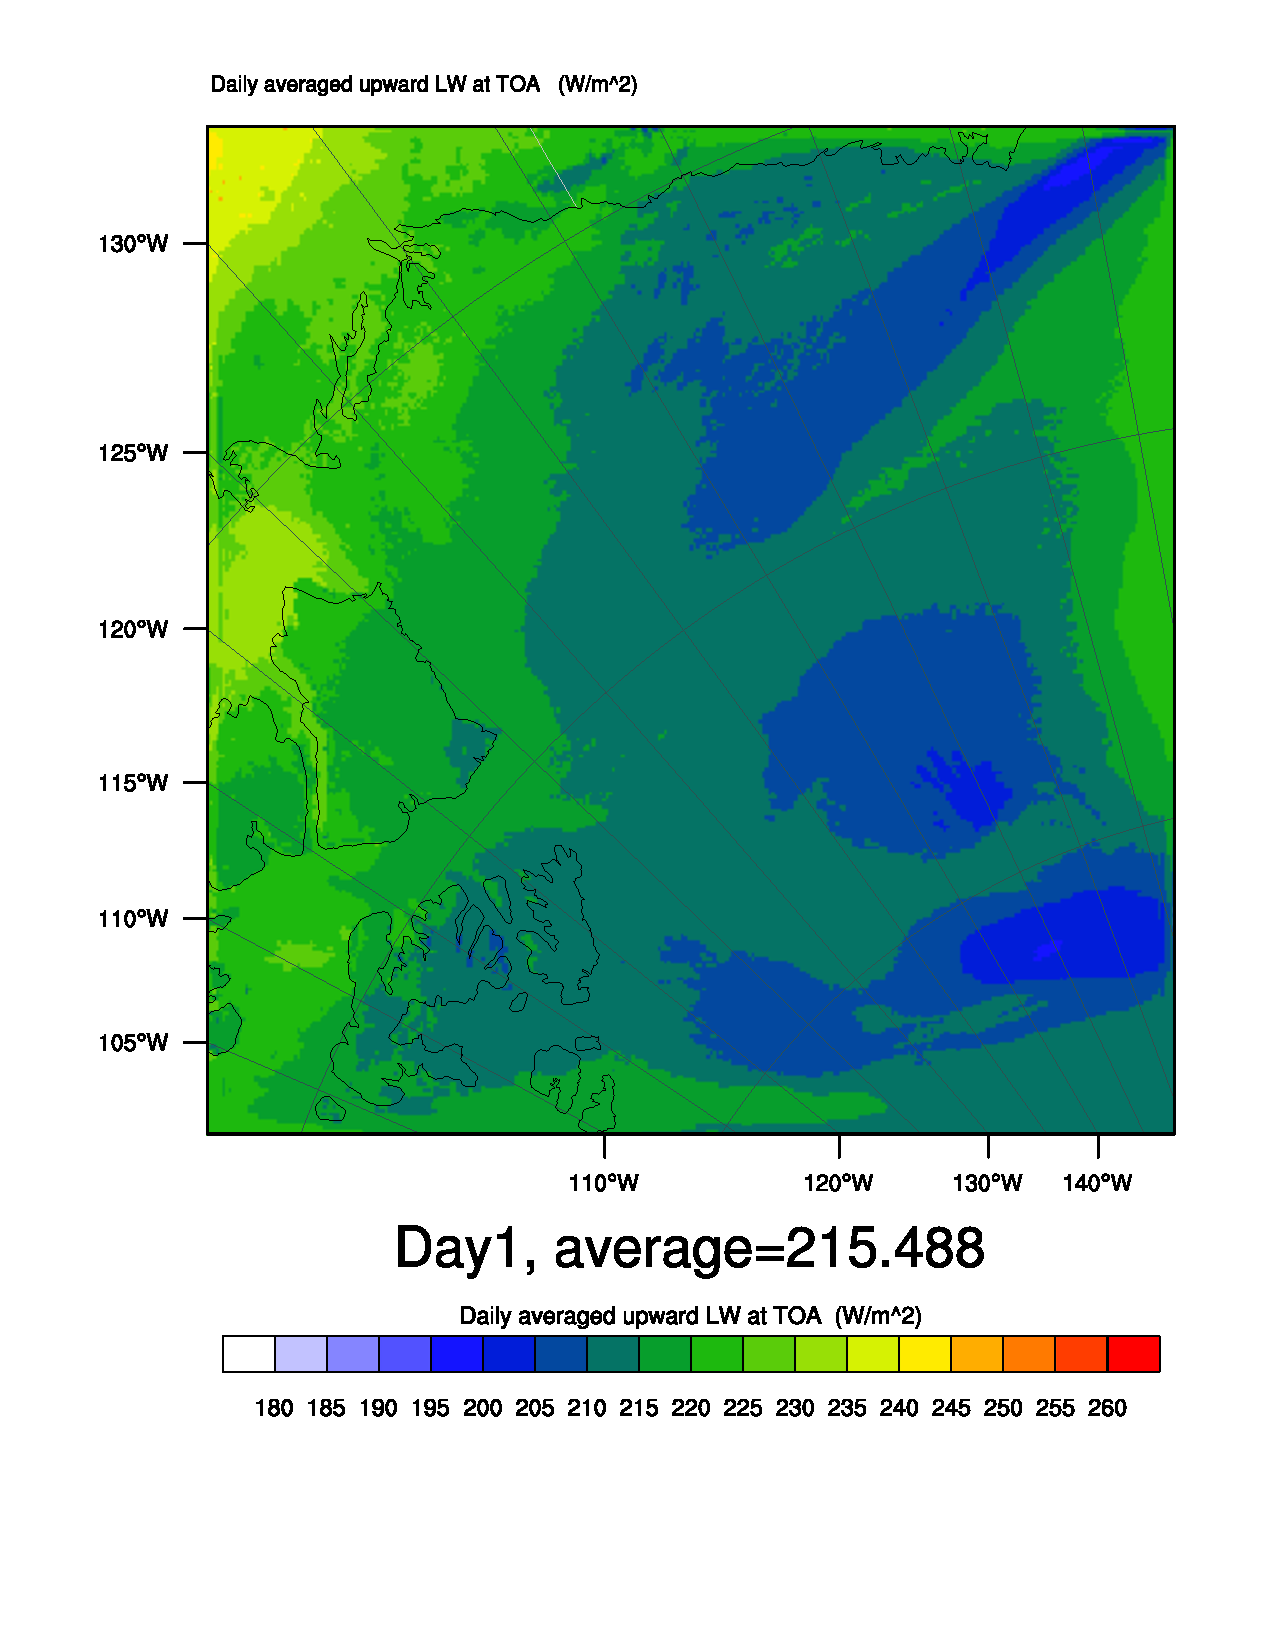
\includegraphics[width=\textwidth]{results/control/LWUPT_Day1.pdf}
		\caption{LW up at TOA, day 1.}
		\label{subfig:lwup_r1Day1}
	\end{subfigure}
	\caption{The average SW and LW flux down at the surface and up at TOA, for day 1. Control.}
	\label{fig:radiation_r1Day1}
\end{figure}

%----- Radiation Day5
\begin{figure}
\centering
	\begin{subfigure}{0.48\textwidth}
		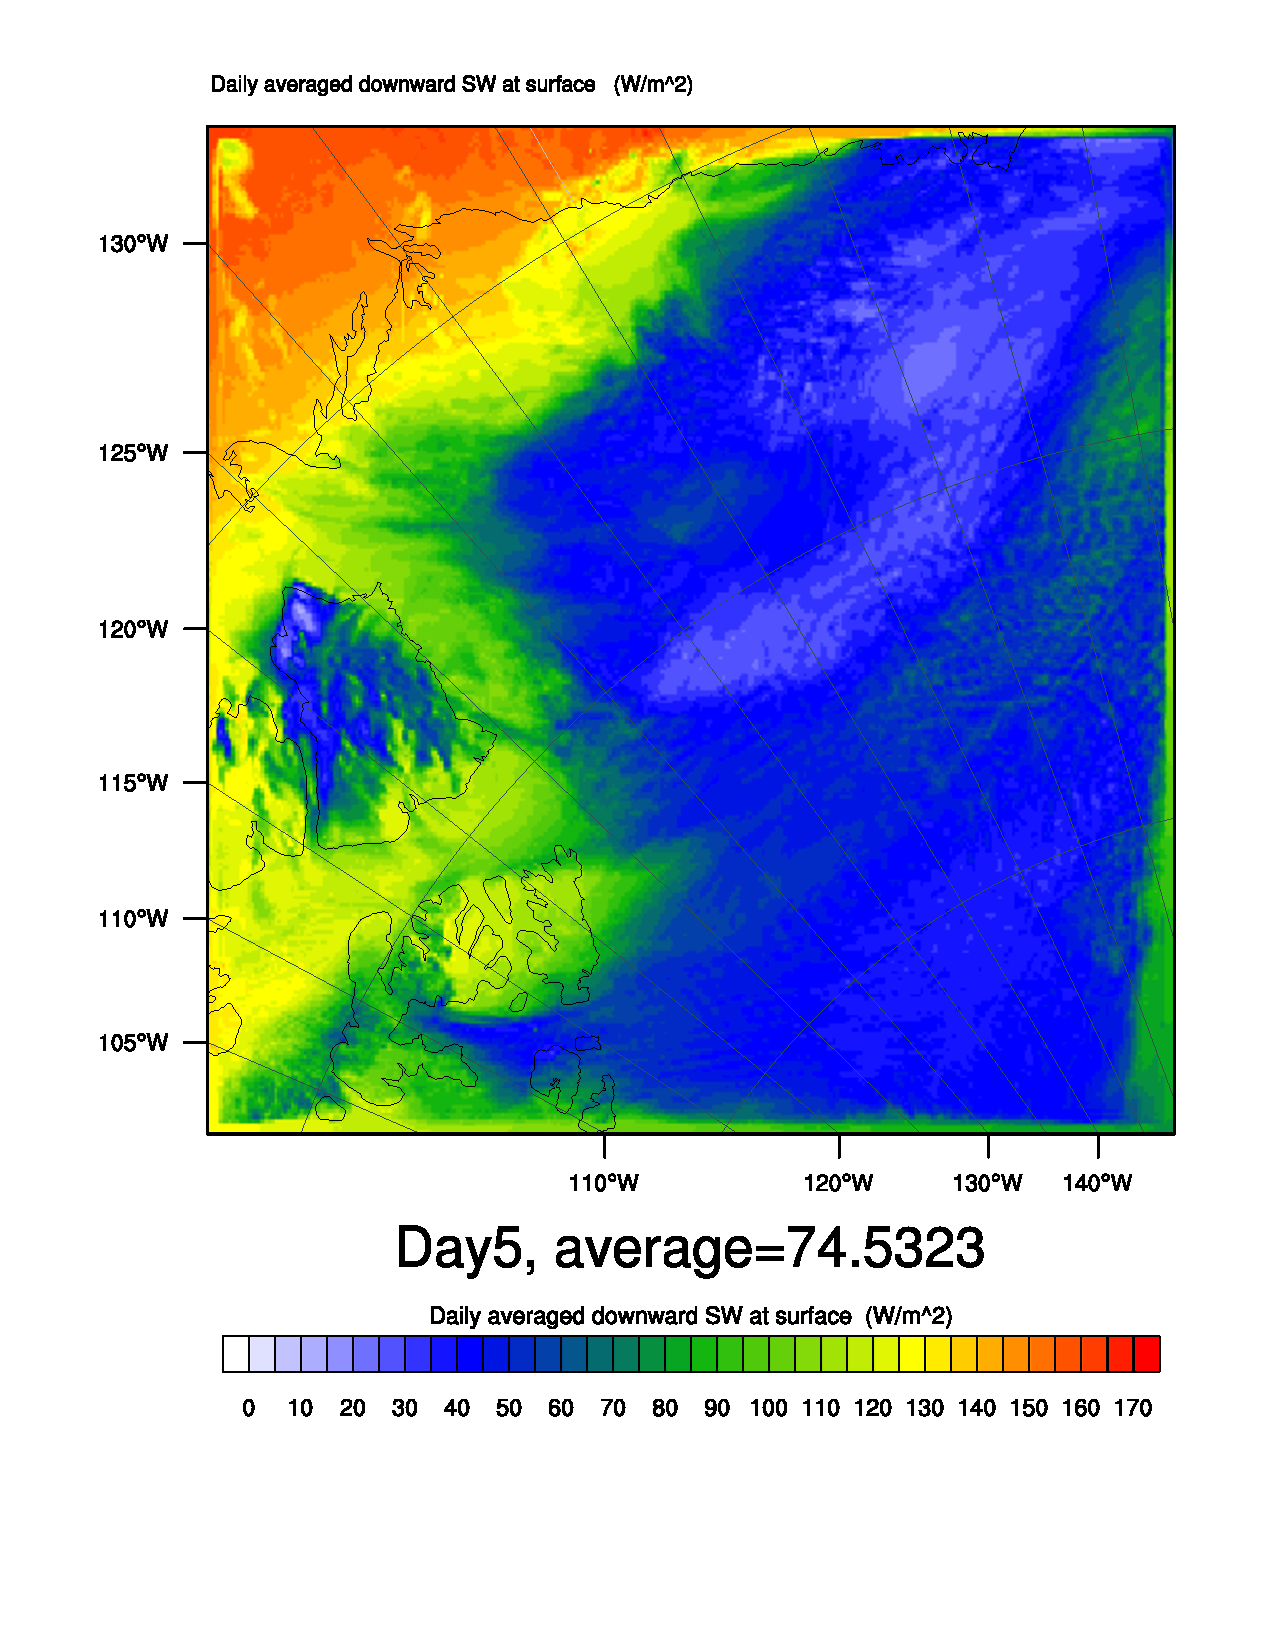
\includegraphics[width=\textwidth]{results/control/SWDOWN_Day5.pdf}
		\caption{The average SW flux down at the surface, day 5.}
		\label{subfig:swdown_r1Day5}
	\end{subfigure}
	\quad
	\begin{subfigure}{0.48\textwidth}
		\centering
		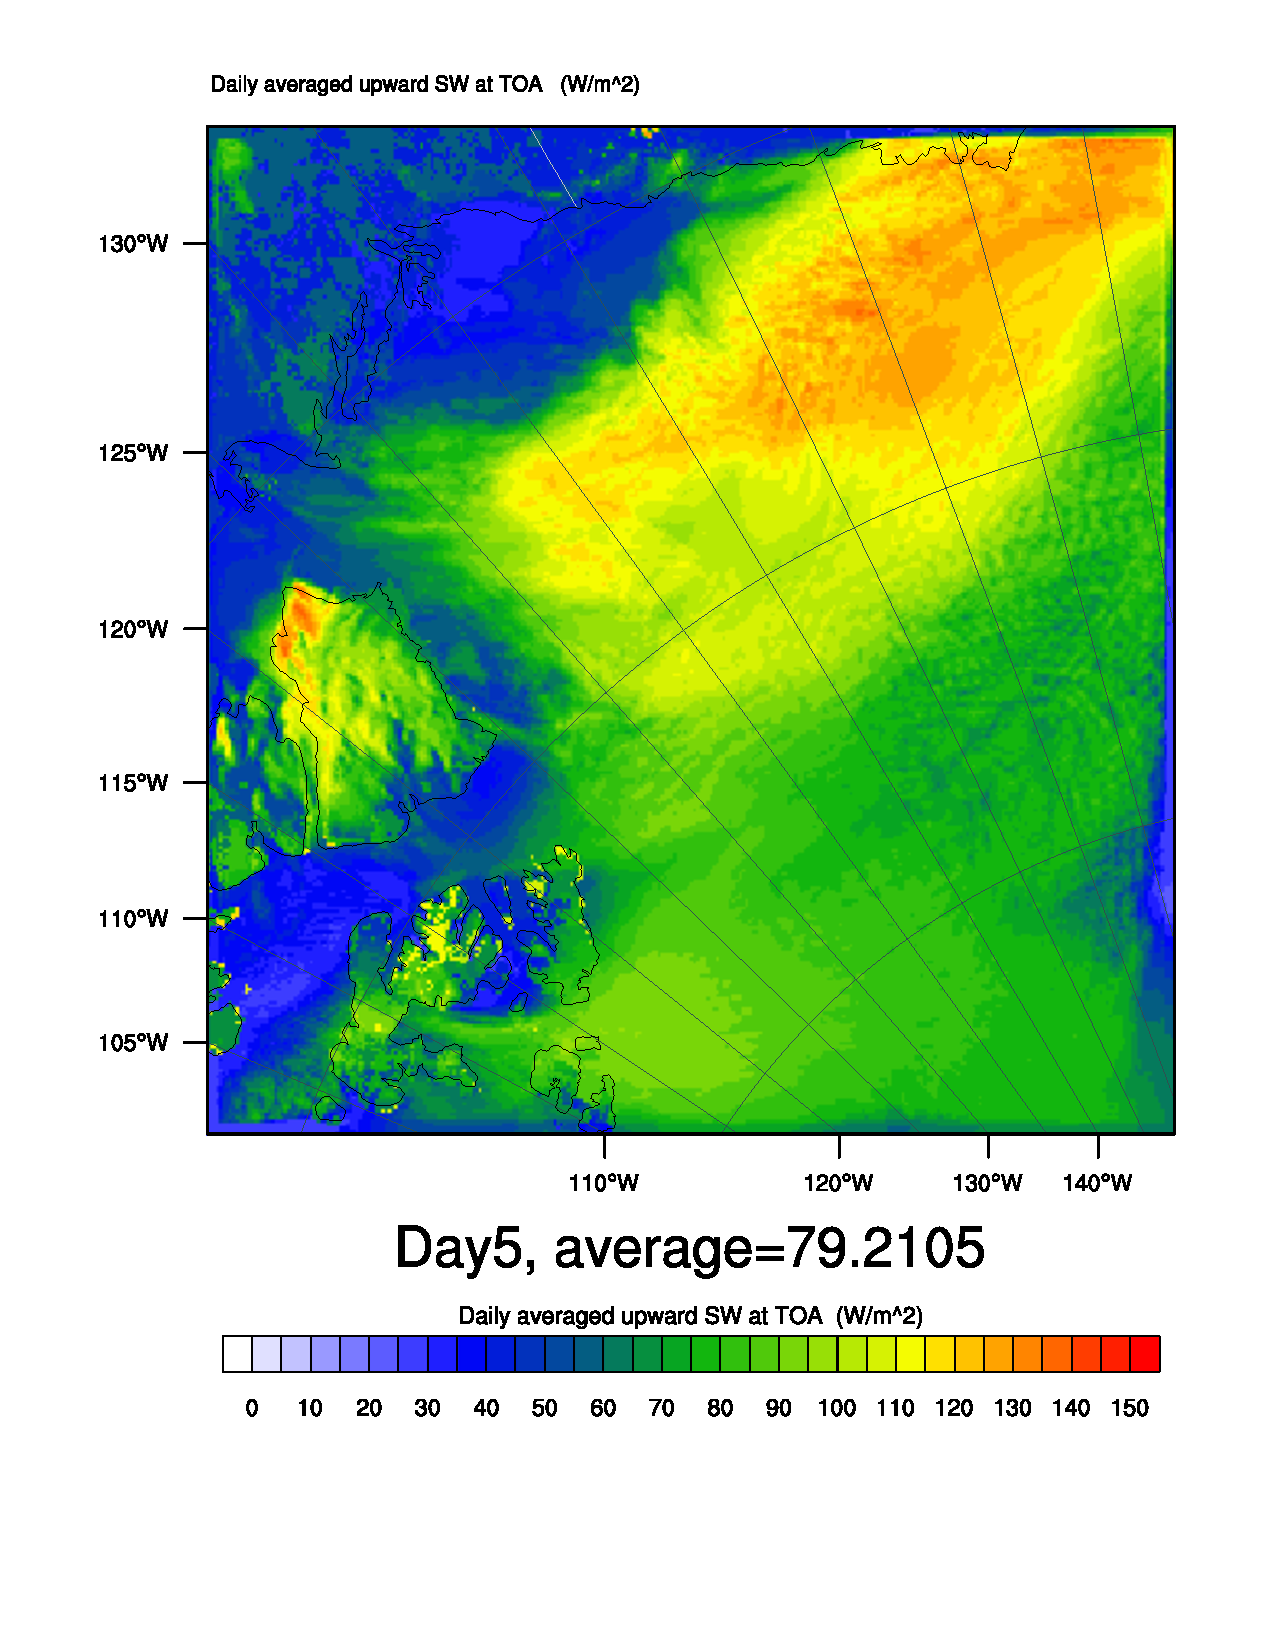
\includegraphics[width=\textwidth]{results/control/SWUPT_Day5.pdf}
		\caption{The average SW flux up at TOA, day 5.}
		\label{subfig:swup_r1Day5}
	\end{subfigure}
	
	\begin{subfigure}{0.48\textwidth}
		\centering
		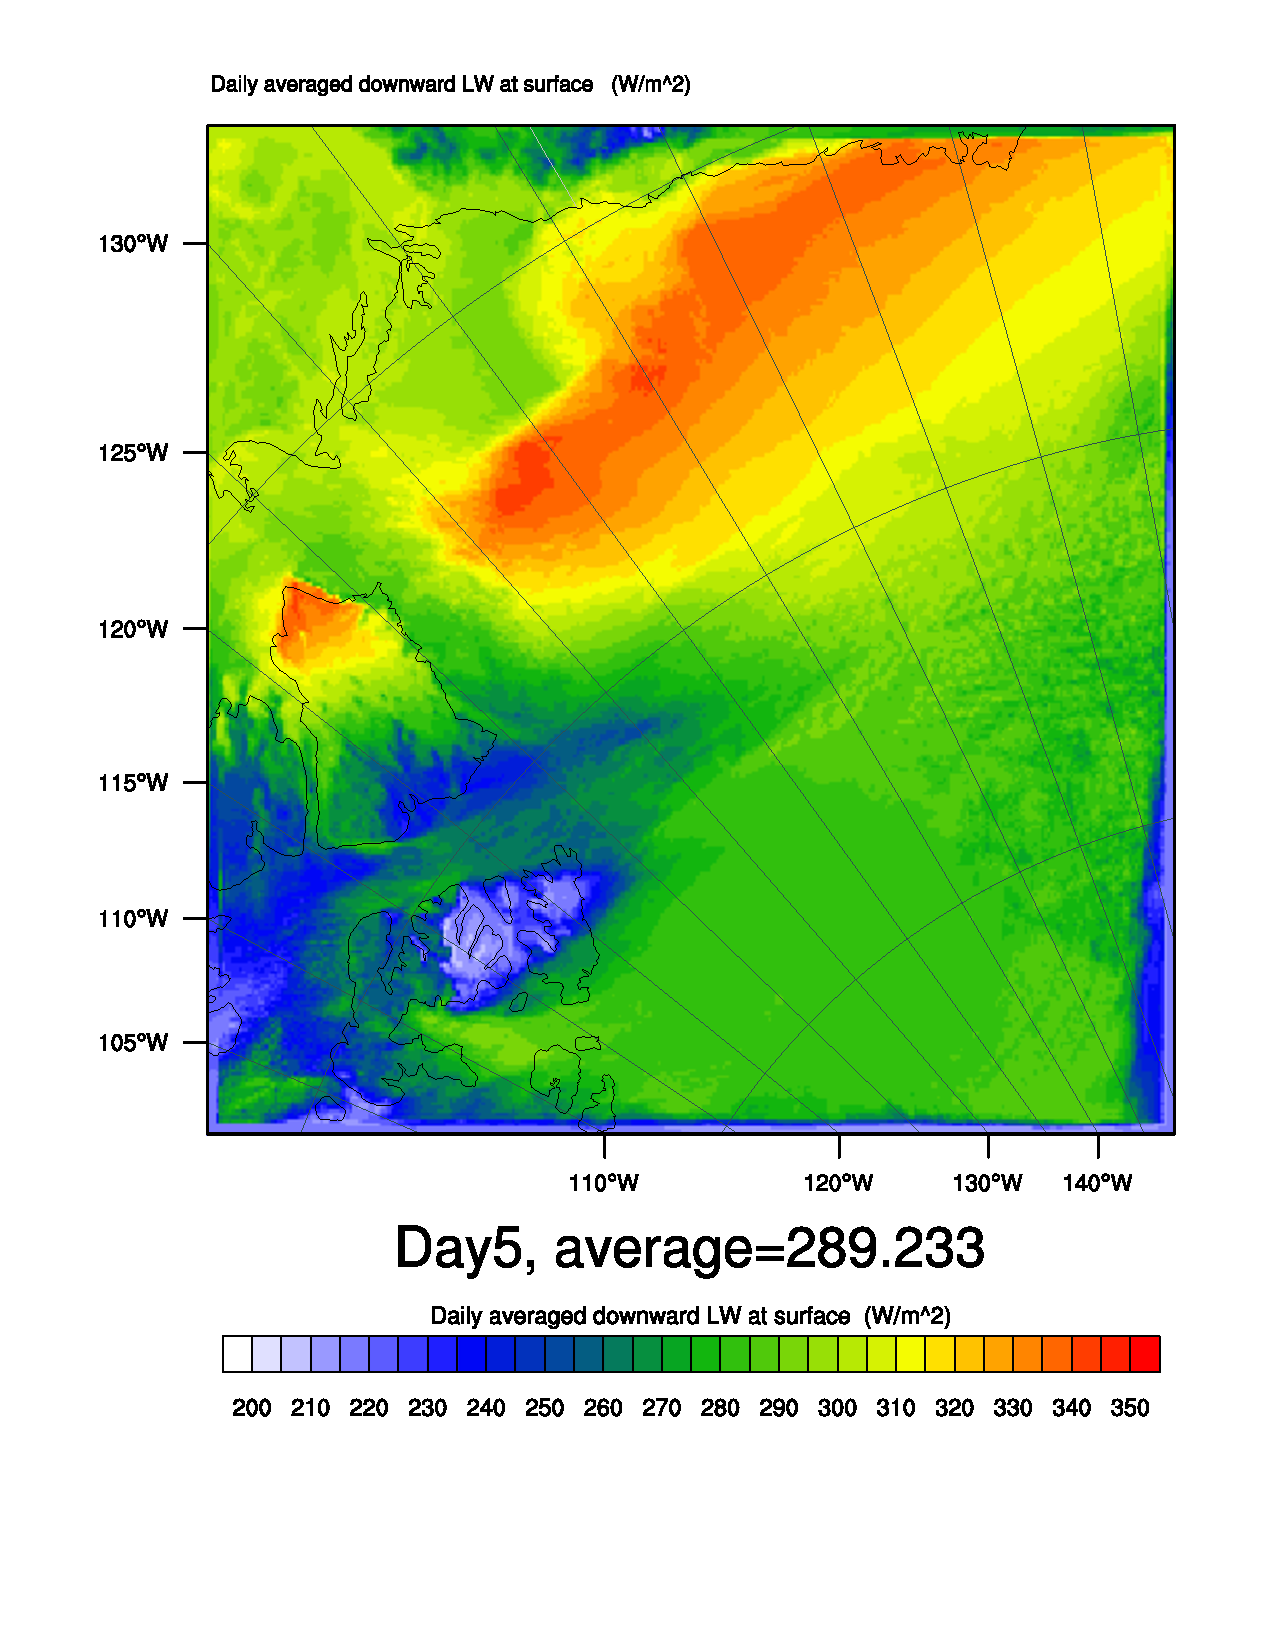
\includegraphics[width=\textwidth]{results/control/GLW_Day5.pdf}
		\caption{The average LW flux down at the surface, day 5.}
		\label{subfig:glw_r1Day5}
	\end{subfigure}
	\quad
	\begin{subfigure}{0.48\textwidth}
		\centering
		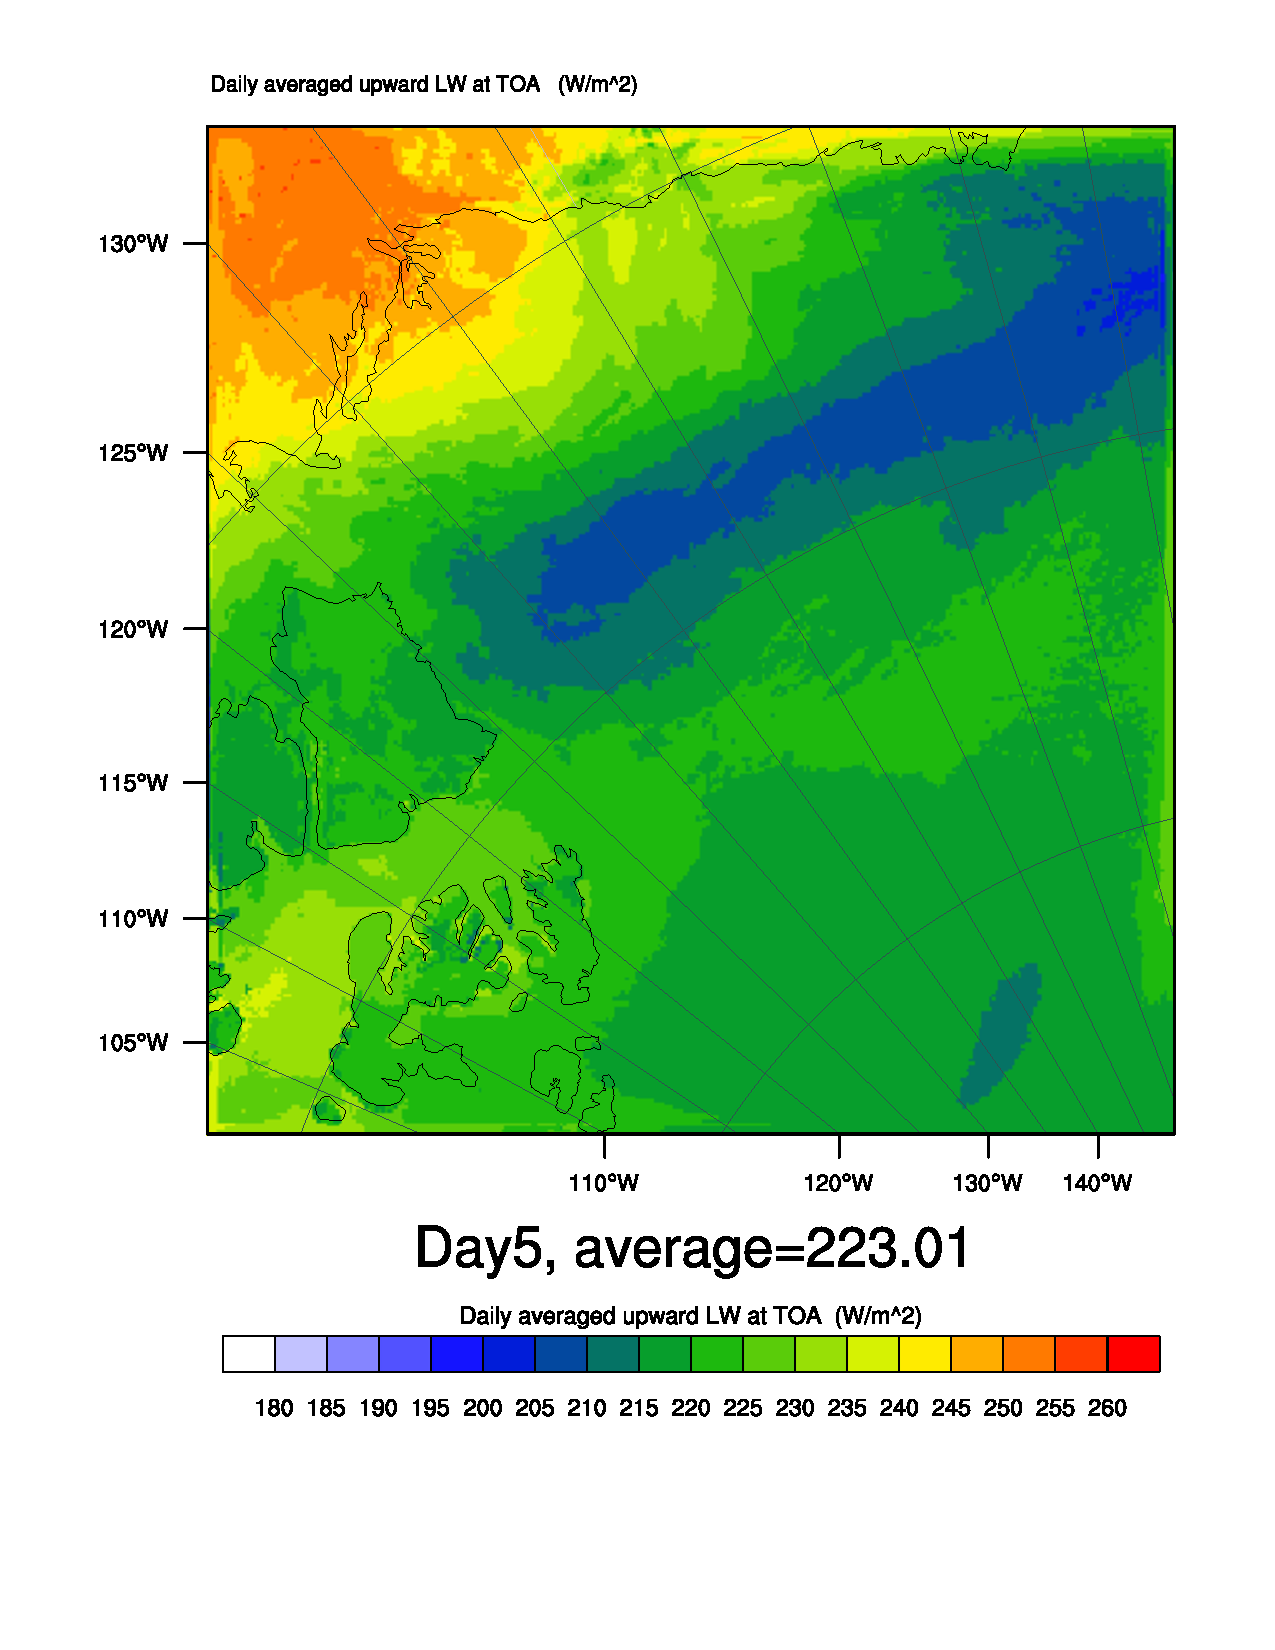
\includegraphics[width=\textwidth]{results/control/LWUPT_Day5.pdf}
		\caption{The average LW flux up at TOA, day 5.}
		\label{subfig:lwup_r1Day5}
	\end{subfigure}
	\caption{The average SW and LW flux down at the surface and up at TOA, for day 5. Control.}
	\label{fig:radiation_r1Day5}
\end{figure}


The heat fluxes upward at the surface, latent heat (LH) and sensible heat (SH), are also of interest when studying clouds in the Arctic. The fluxes are shown in figure~\ref{fig:surface_fluxes_r1} for days 1 and 5. Notice that the LH is lower over the sea ice for both days 1 and 5. This because the sea ice is colder than the ocean, and works as a lid over that part of the ocean, not letting all the heat and water vapor out. Another thing to notice is the marked increase in SH just off the sea ice edge, 77$\degree$N, 135$\degree$W, day 5. This is due to the strong winds in that area (figure~\ref{subfig:weather_cont_day5}), which brings cold air from over the ice out over the warmer open ocean. Thus the temperature gradient is stronger just off the sea ice edge, increasing the heat given to from the surface to the overlying air. The effect is strongest at the sea ice edge, but is also evident further away over the ocean, to about 160$\degree$W. The reason the effect stretches so far is the wind speed, which is just above 10~$\text{m/s}$ (see figure~\ref{subfig:weather_cont_day5}).

%----- Surface heat fluxes
\begin{figure}
\centering
	\begin{subfigure}{0.48\textwidth}
		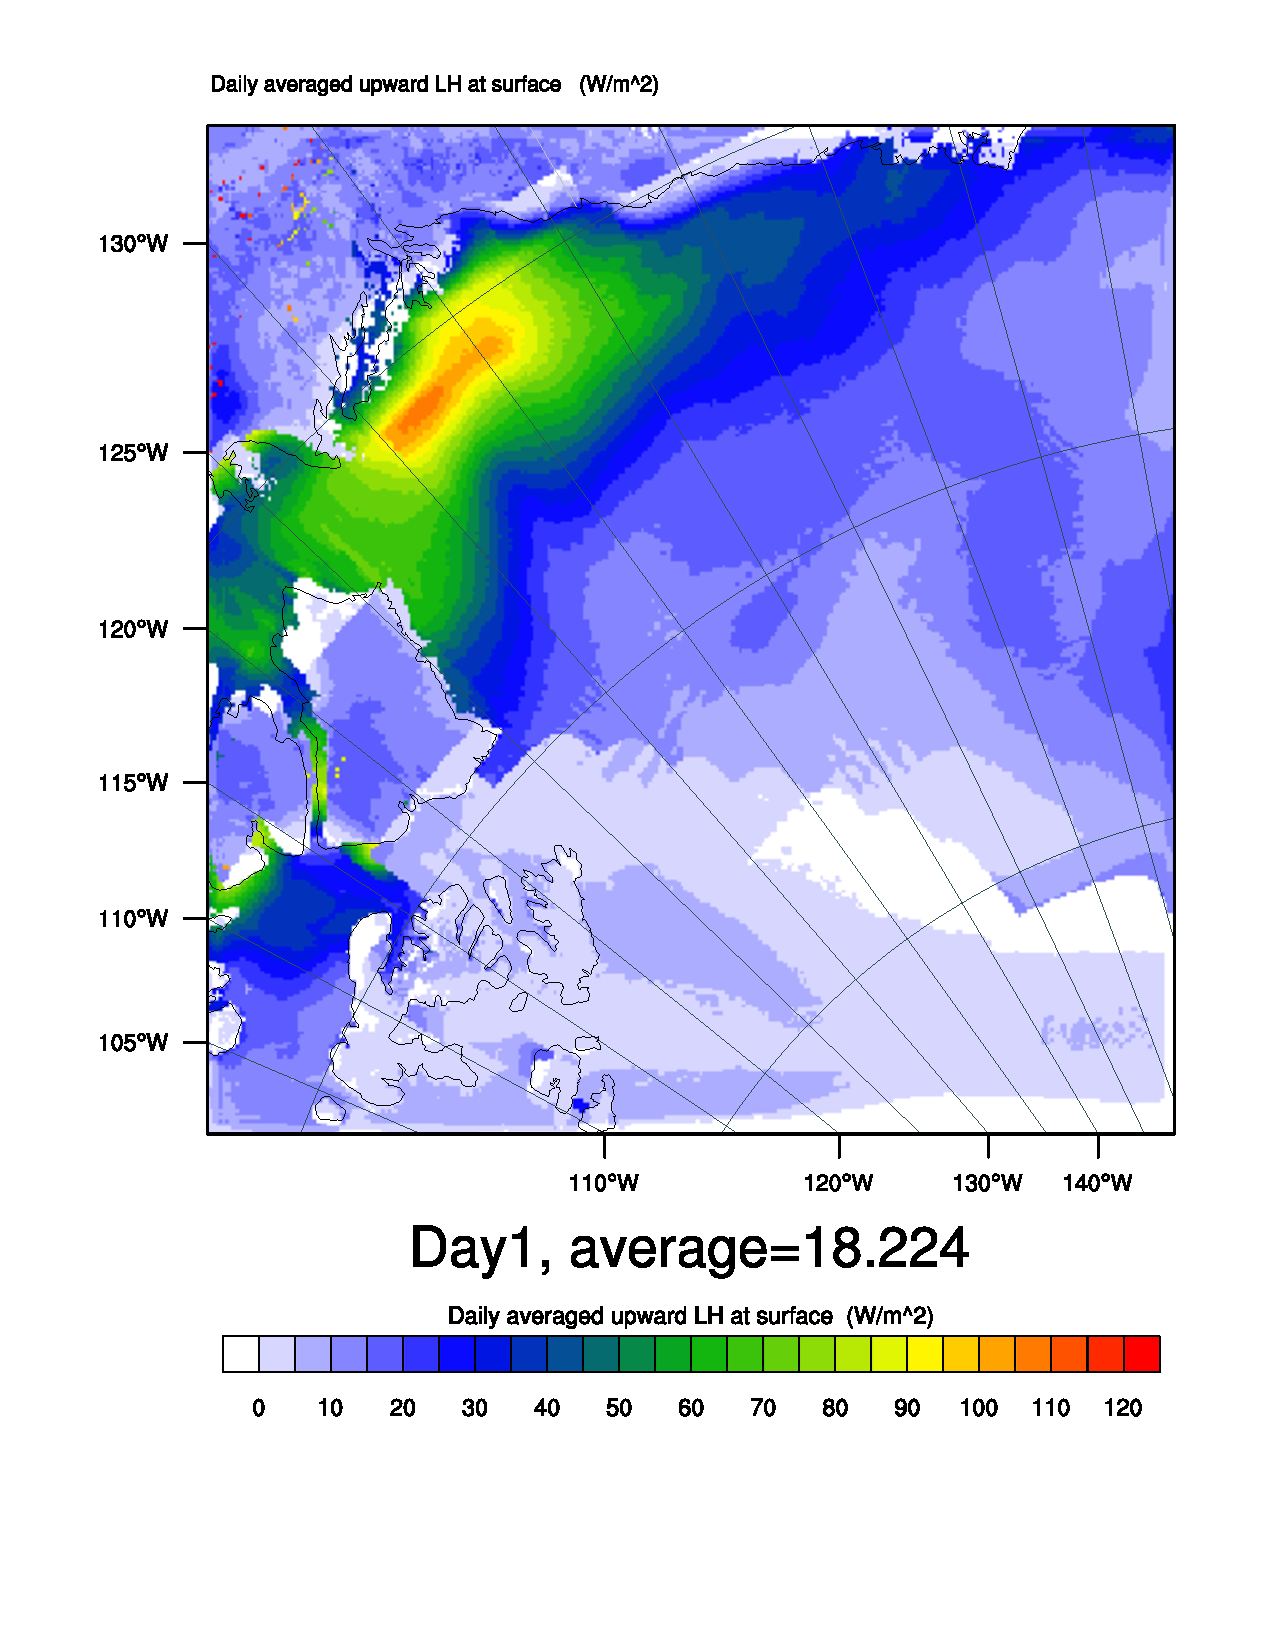
\includegraphics[width=\textwidth]{results/control/LH_Day1.pdf}
		\caption{LH day 1.}
		\label{subfig:lh_r1Day1}
	\end{subfigure}
	\quad
	\begin{subfigure}{0.48\textwidth}
		\centering
		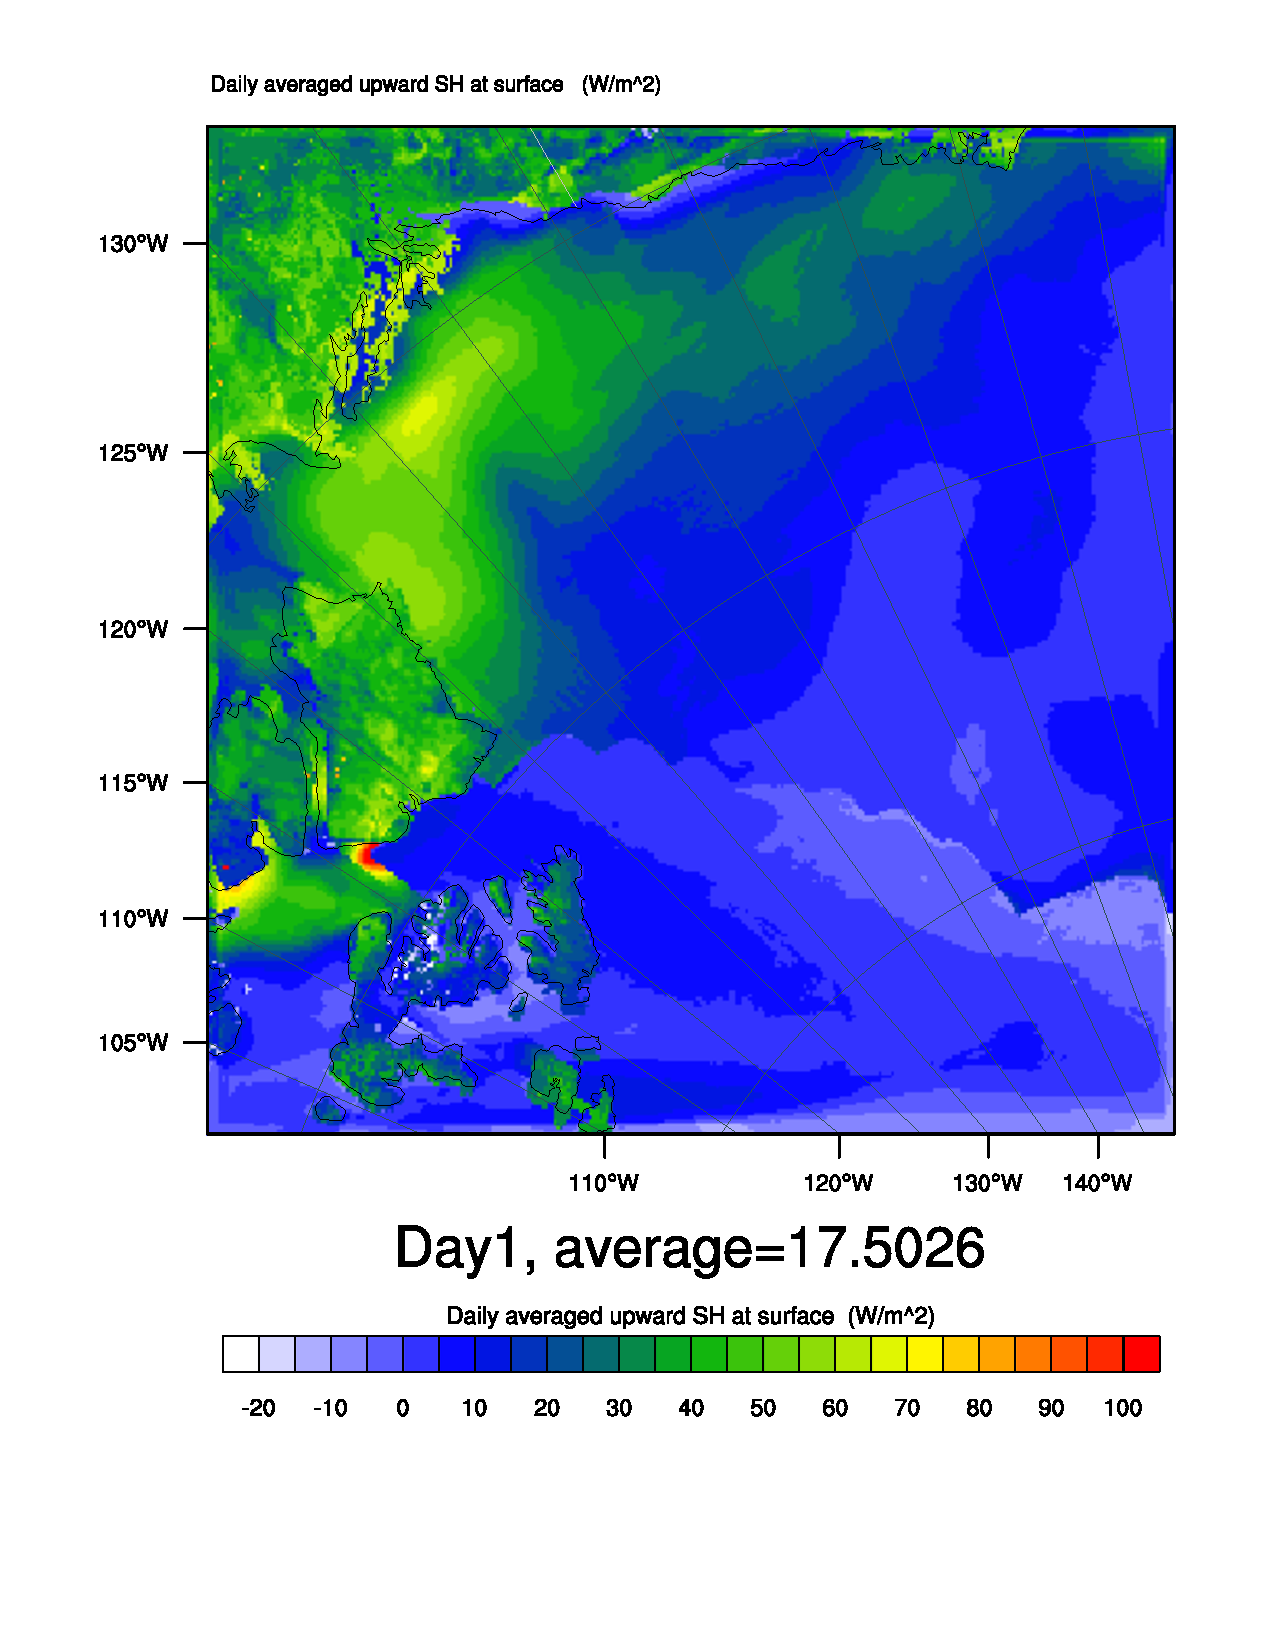
\includegraphics[width=\textwidth]{results/control/HFX_Day1.pdf}
		\caption{SH day 1.}
		\label{subfig:sh_r1Day1}
	\end{subfigure}
	
	\begin{subfigure}{0.48\textwidth}
		\centering
		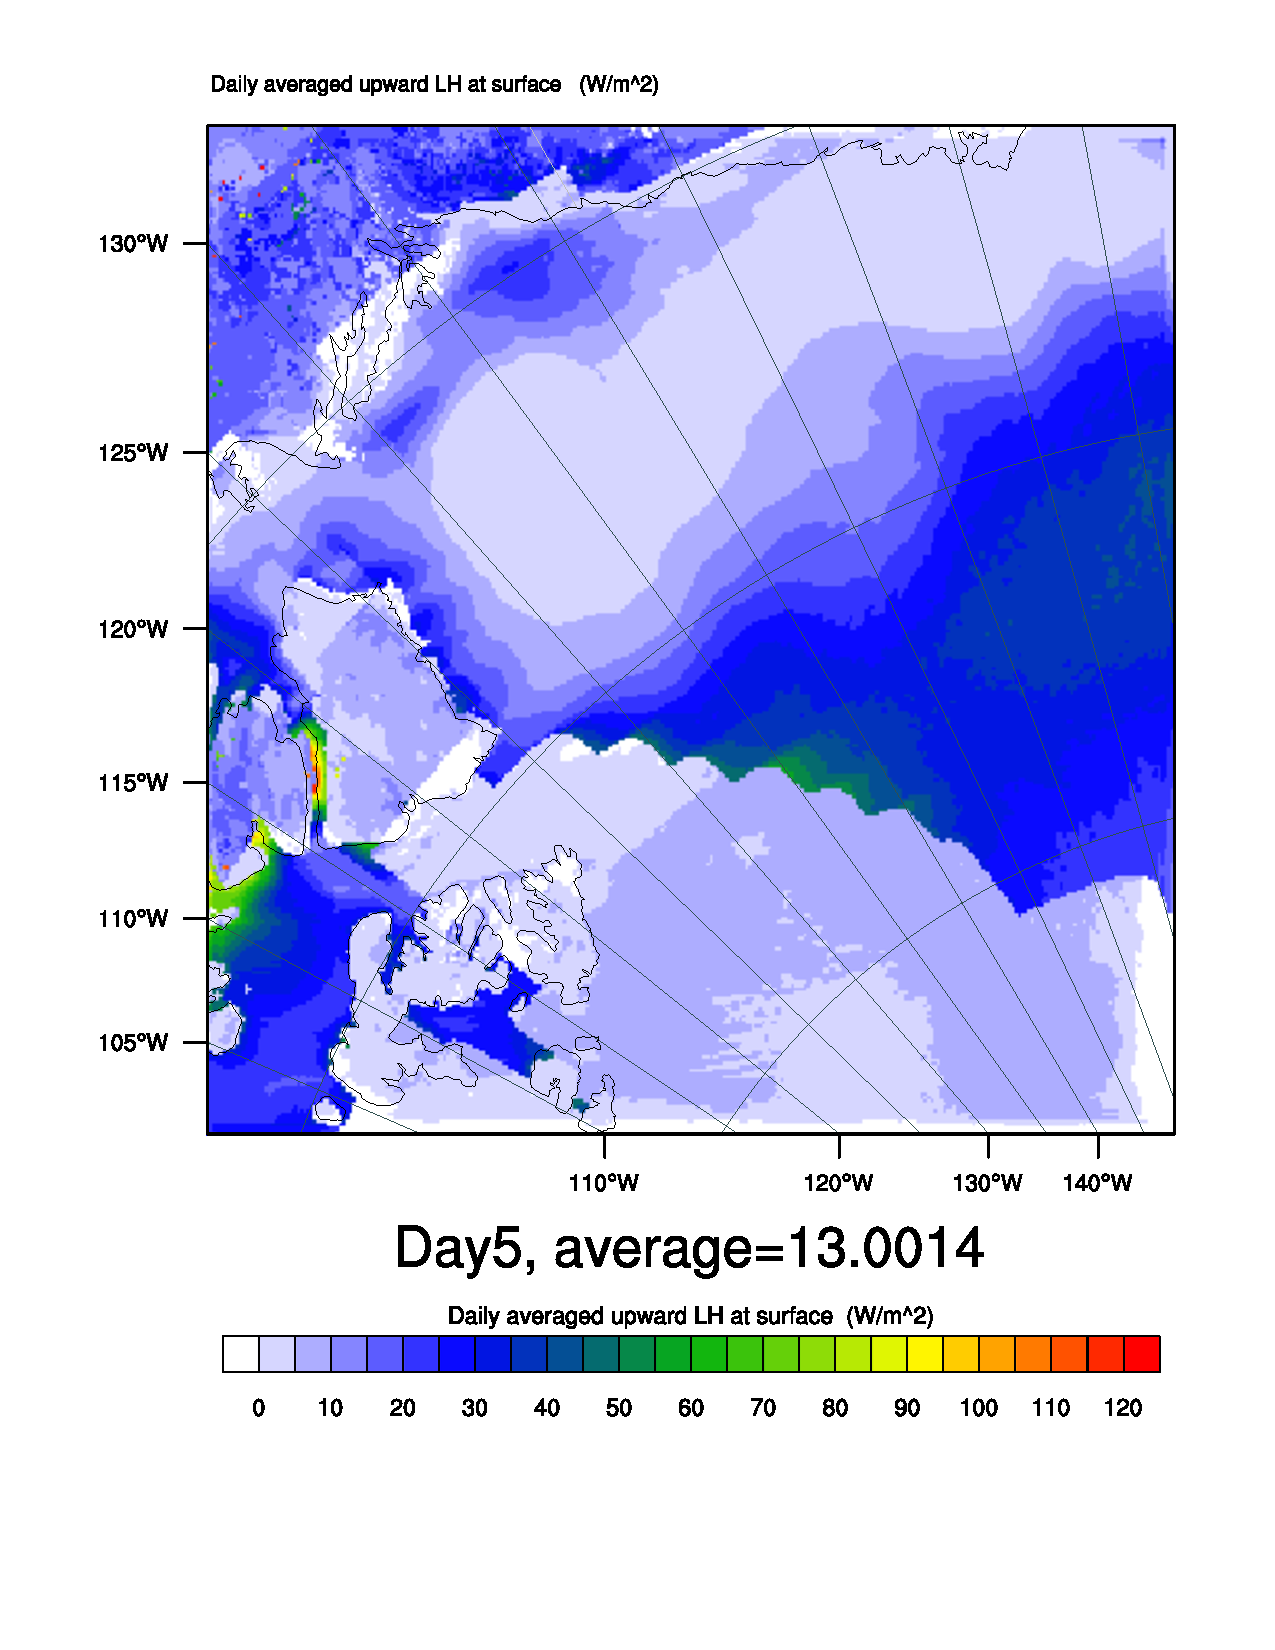
\includegraphics[width=\textwidth]{results/control/LH_Day5.pdf}
		\caption{LH day 5.}
		\label{subfig:lh_r1Day5}
	\end{subfigure}
	\quad
	\begin{subfigure}{0.48\textwidth}
		\centering
		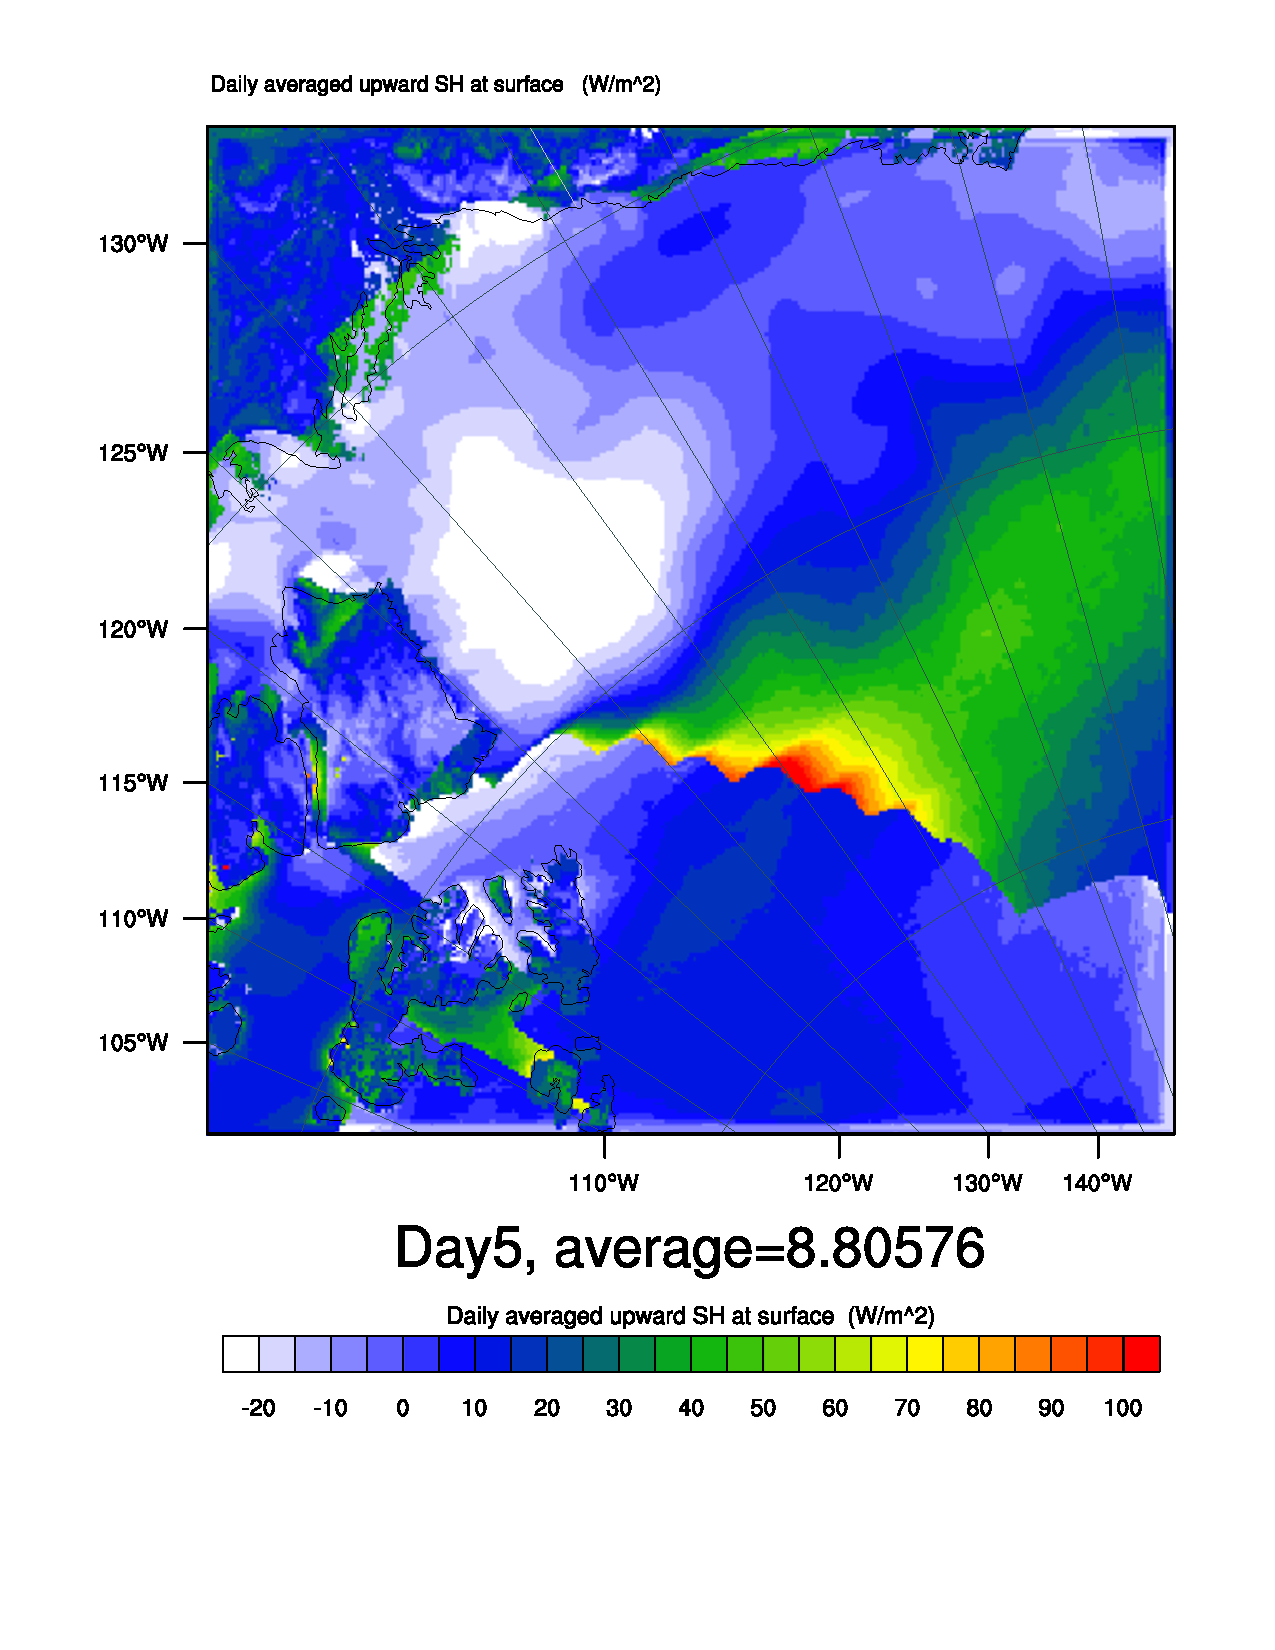
\includegraphics[width=\textwidth]{results/control/HFX_Day5.pdf}
		\caption{SH day 5.}
		\label{subfig:sh_r1Day5}
	\end{subfigure}
	\caption{The average surface heat fluxes (SH and LH) up at the surface, for days 1 and 5. Control.}
	\label{fig:surface_fluxes_r1}
\end{figure}

%--------- Skin temperature
\begin{figure}
	\begin{subfigure}{0.48\textwidth}
		\centering
		\includegraphics[width=\textwidth]{results/control/skintemp_day1.pdf}
		\caption{Day 1}
		\label{subfig:skin_r1Day1}
	\end{subfigure}
	\begin{subfigure}{0.48\textwidth}
		\centering
		\includegraphics[width=\textwidth]{results/control/skintemp_day5.pdf}
		\caption{Day 5}
		\label{subfig:skin_r1Day5}
	\end{subfigure}
	\caption{Daily averaged skin temperature (K) of the study area, for both days 1 and 5. Control.}
	\label{fig:skintemp}
\end{figure}

%-------------------------------
\clearpage
\section{Removed sea ice}
%-------------------------------
The sea ice was removed to study the effect this had on the cloud radiative properties, and through that if it had heating or cooling effects at the surface. @\textit{Explain why sea ice was removed, repeat stuff from earlier!} The sea ice that was present in the control run, but has been removed for NoIce, is shown in figure~\ref{fig:seaice}. 

\begin{figure}[hb]
\centering
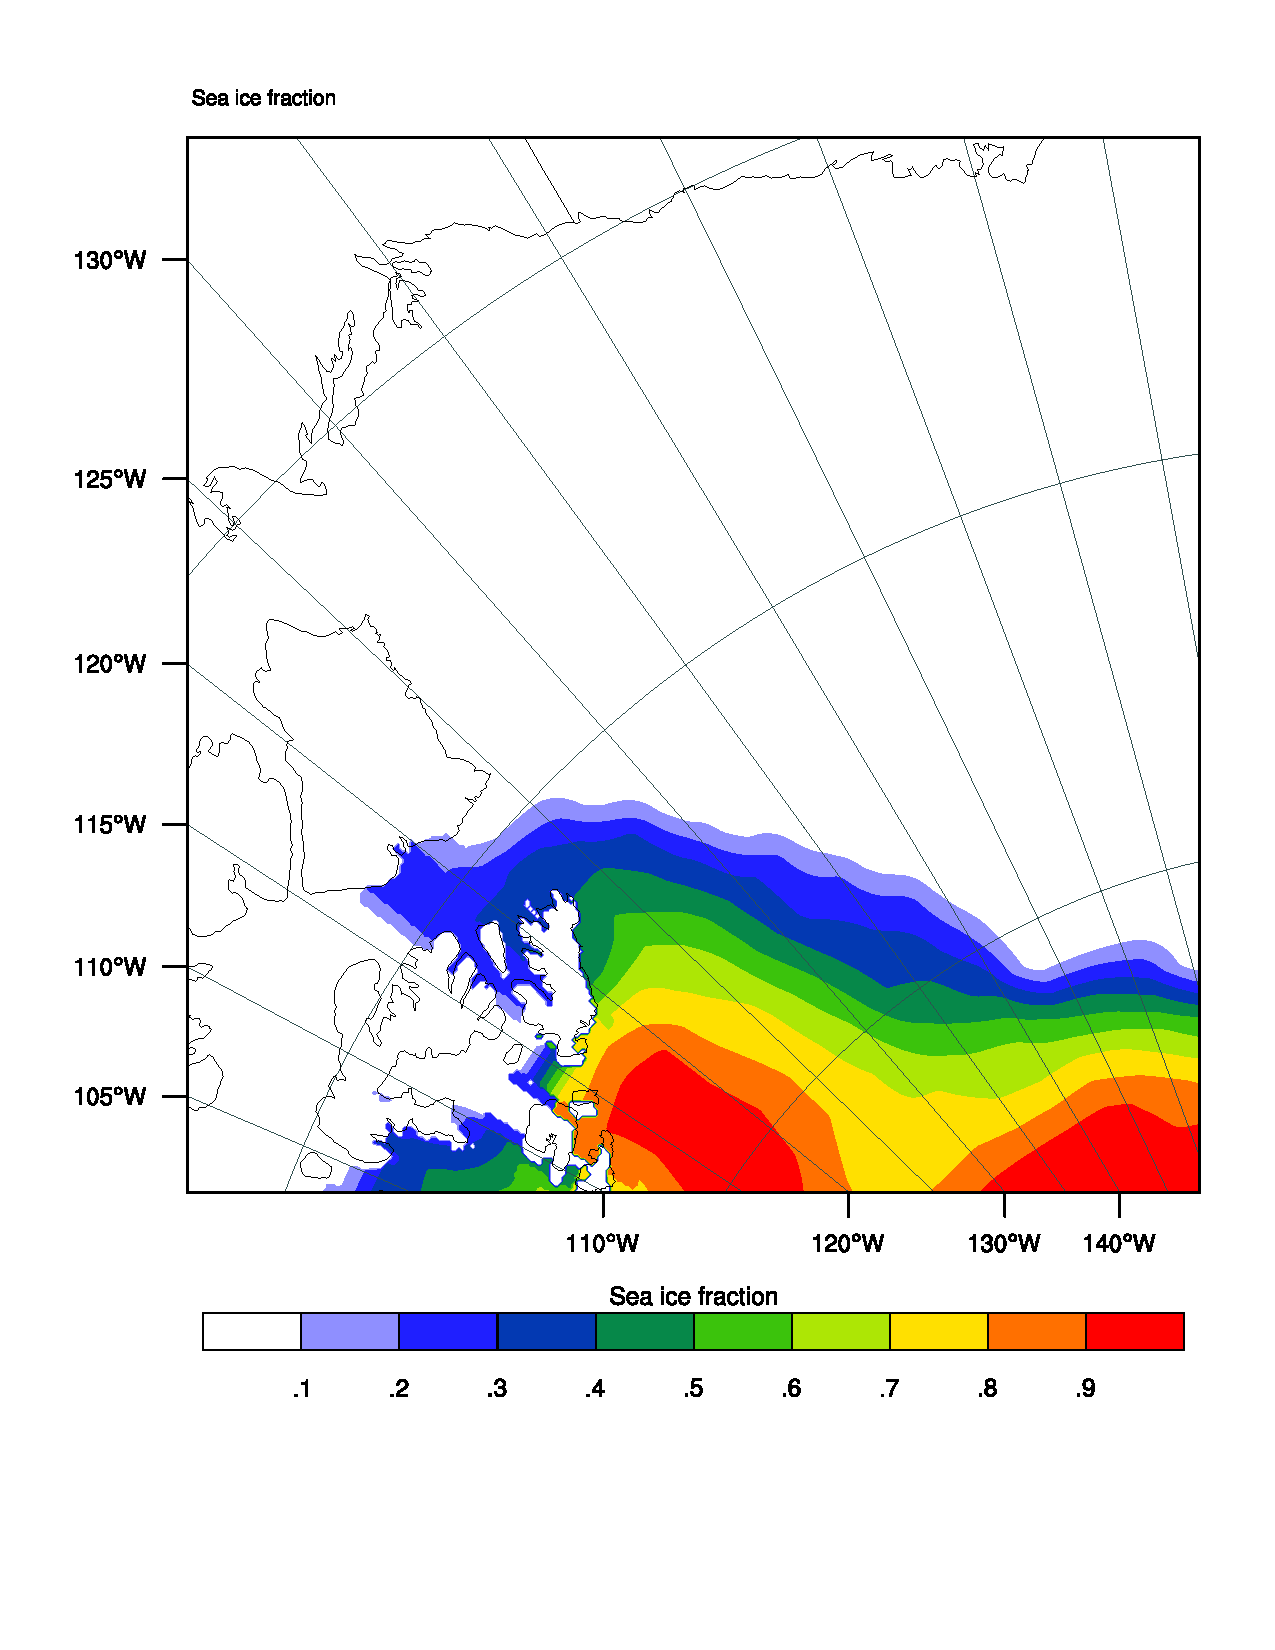
\includegraphics[width=0.5\textwidth]{results/control/seaiceplot.pdf}
\caption{Sea ice fraction in Control (and Aero10).}
\label{fig:seaice}
\end{figure}

\subsection{Day 1}
\label{sec:noiceDay1}
The average difference in LWP, NoIce-Control, for day 1, shown in figure~\ref{subfig:LWPr2Day1} is small (@??) for the whole field ($\sim$0.23~$\text{g/m}^2$ increase). But the area of interest in this case is where the sea ice is not present, which it was in the control run (figure~\ref{fig:seaice}). The sea ice edge is also included as a black contour in figure~\ref{subfig:cross_line}. The area where there was sea ice in the control run shows a positive difference in LWP. Especially furthest north (bottom right corner of the map) the LWP is significantly higher, >15~$\text{g/m}^2$.

\begin{figure}
\centering
	\begin{subfigure}{0.40\textwidth}
		\centering
		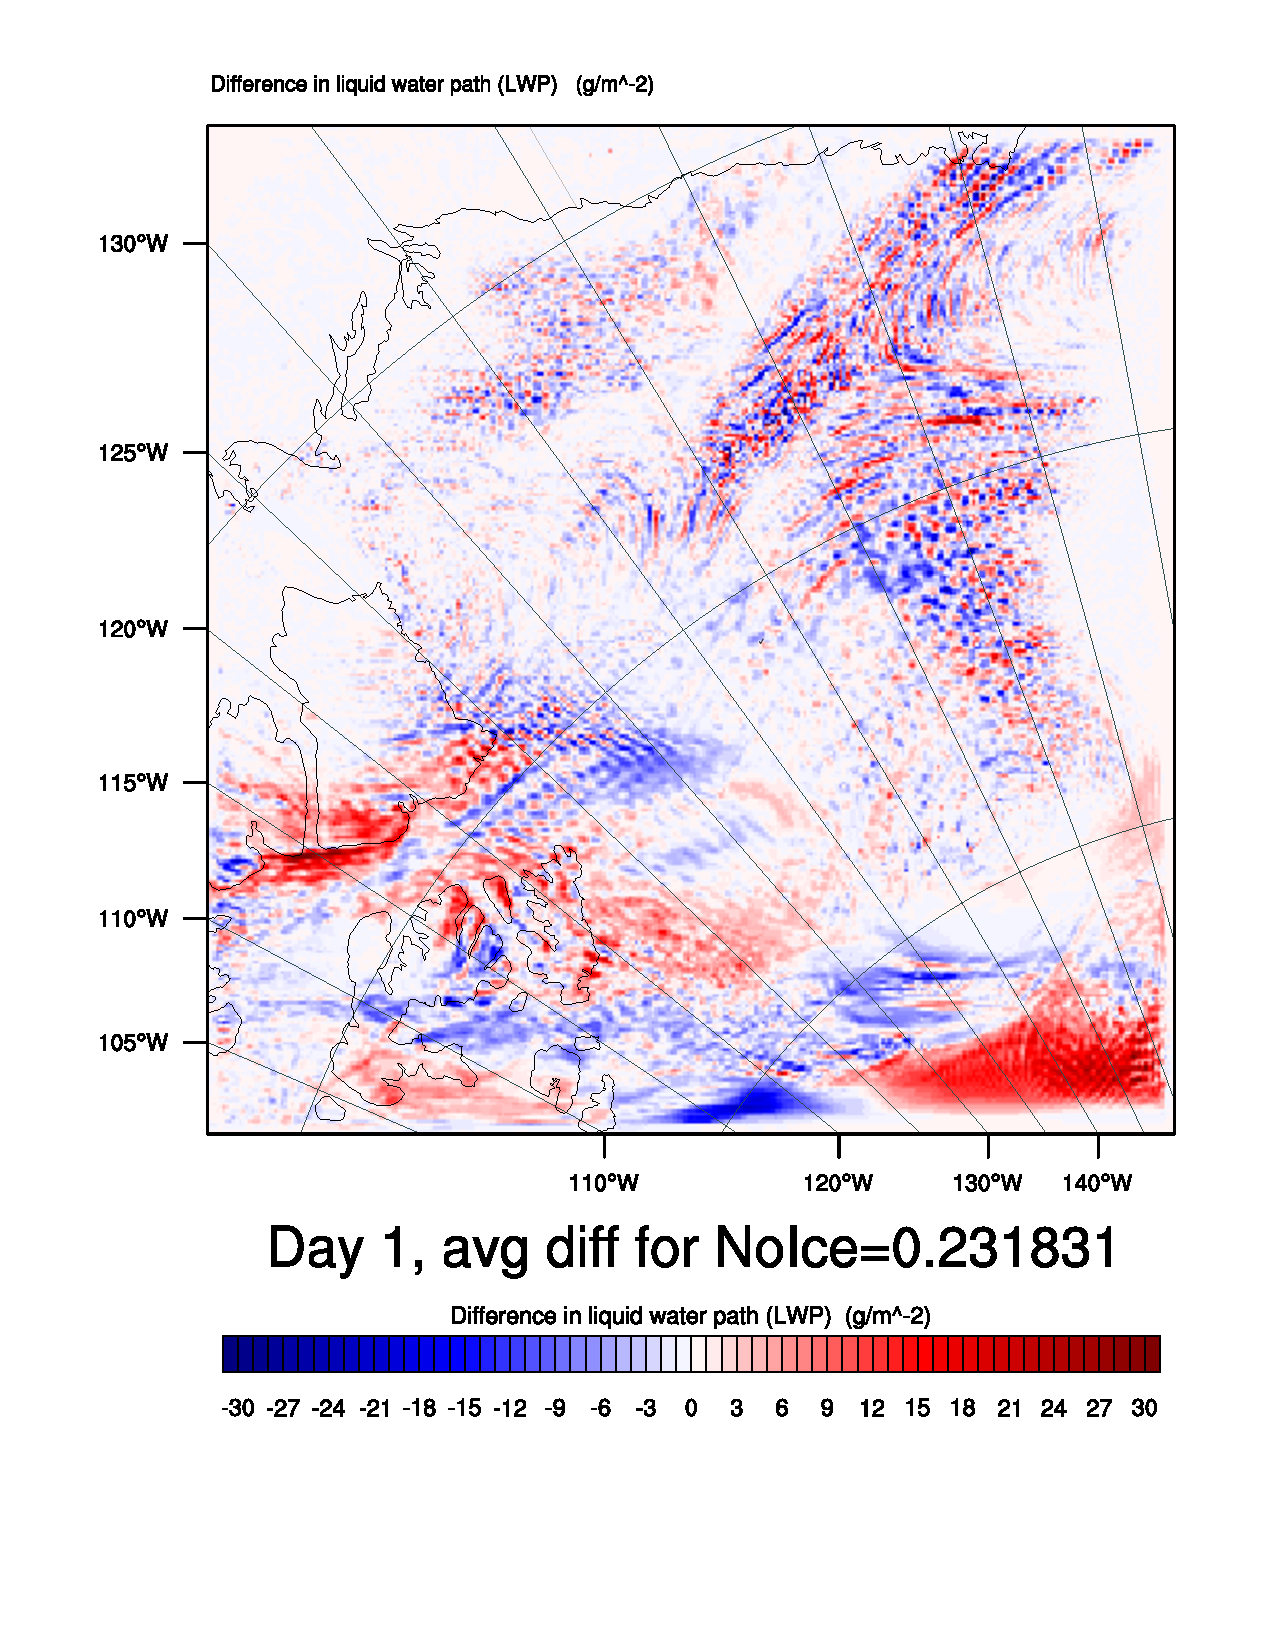
\includegraphics[width=\textwidth]{results/noice/Diff_LWP_Day1NoIce.pdf}
		\caption{LWP, NoIce, day 1}
		\label{subfig:LWPr2Day1}
	\end{subfigure}
	\quad
	\begin{subfigure}{0.40\textwidth}
		\centering
		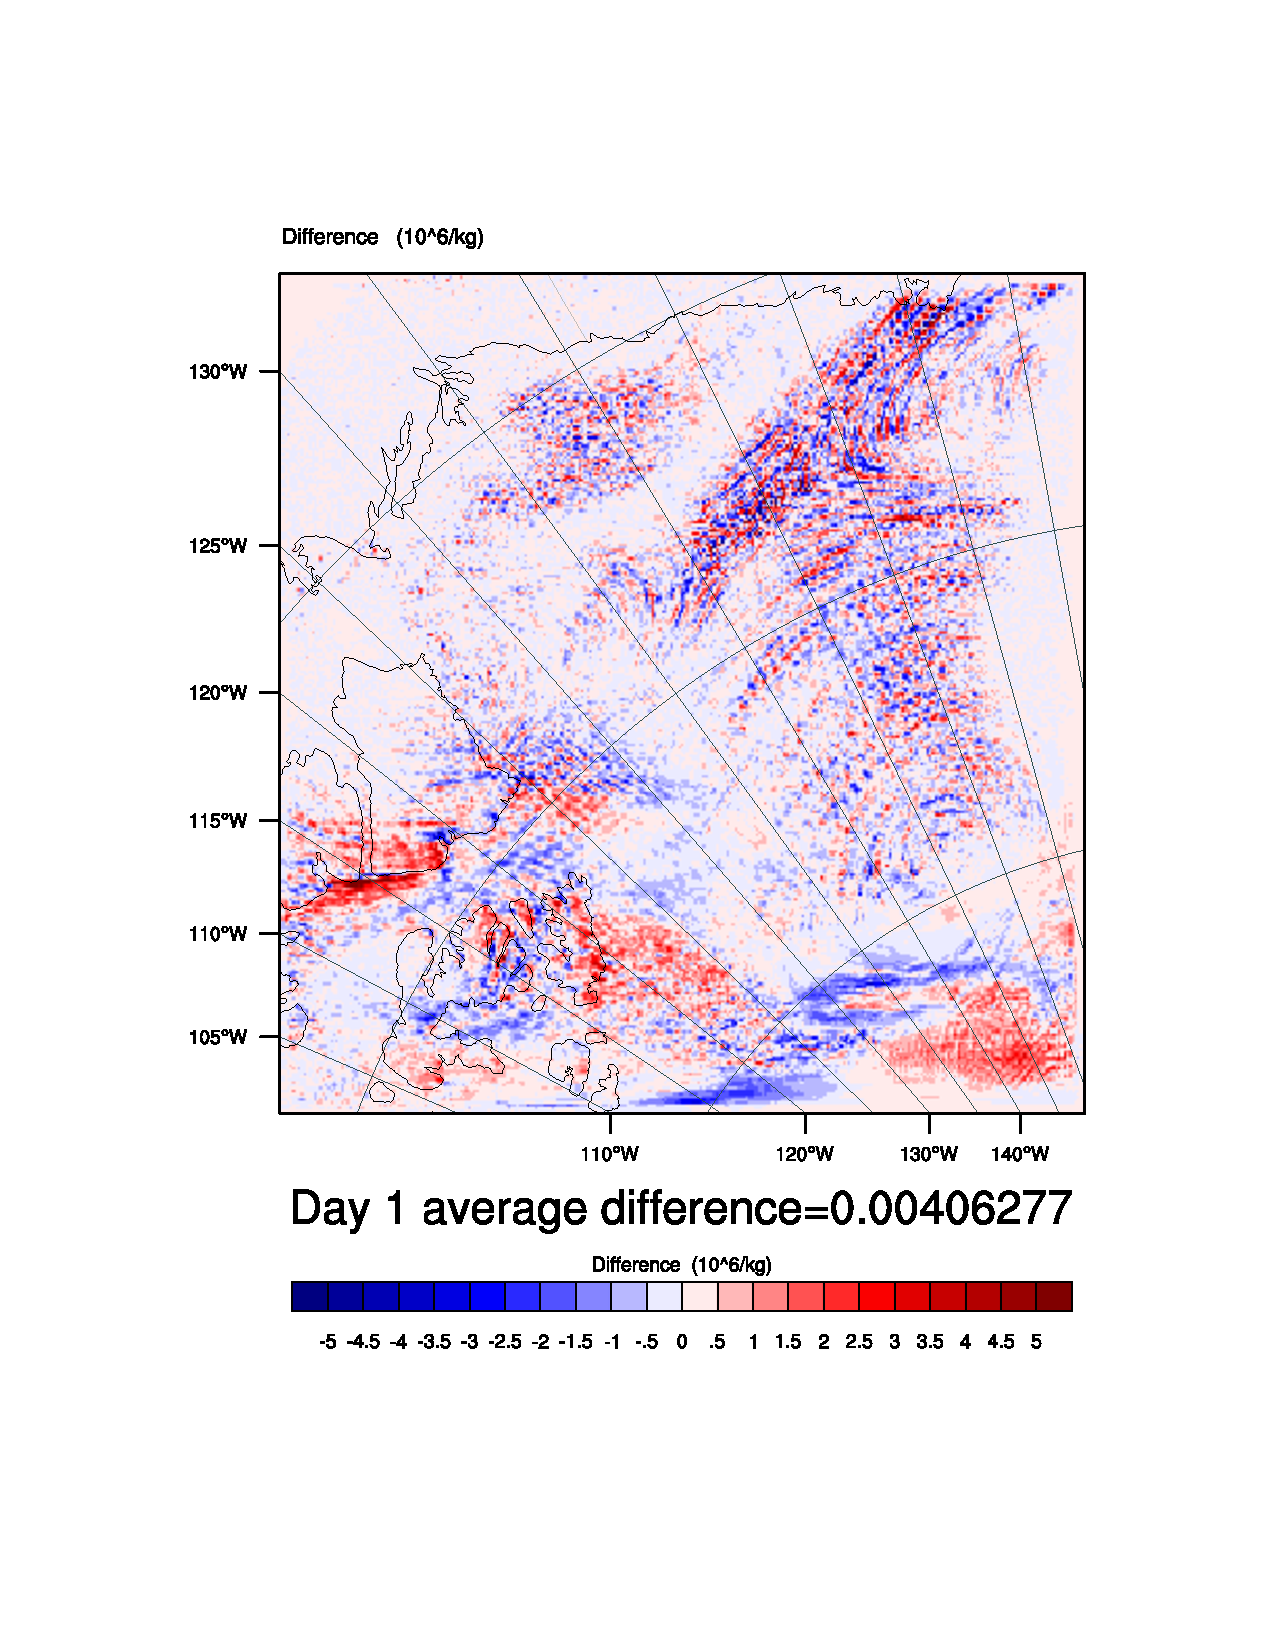
\includegraphics[width=\textwidth]{results/noice/diff_NoIce_QNCLOUD_Day1.pdf}
		\caption{CDNC, NoIce, day 1}
		\label{subfig:CDNCr2Day1}
	\end{subfigure}
	
	\begin{subfigure}{0.40\textwidth}
		\centering
		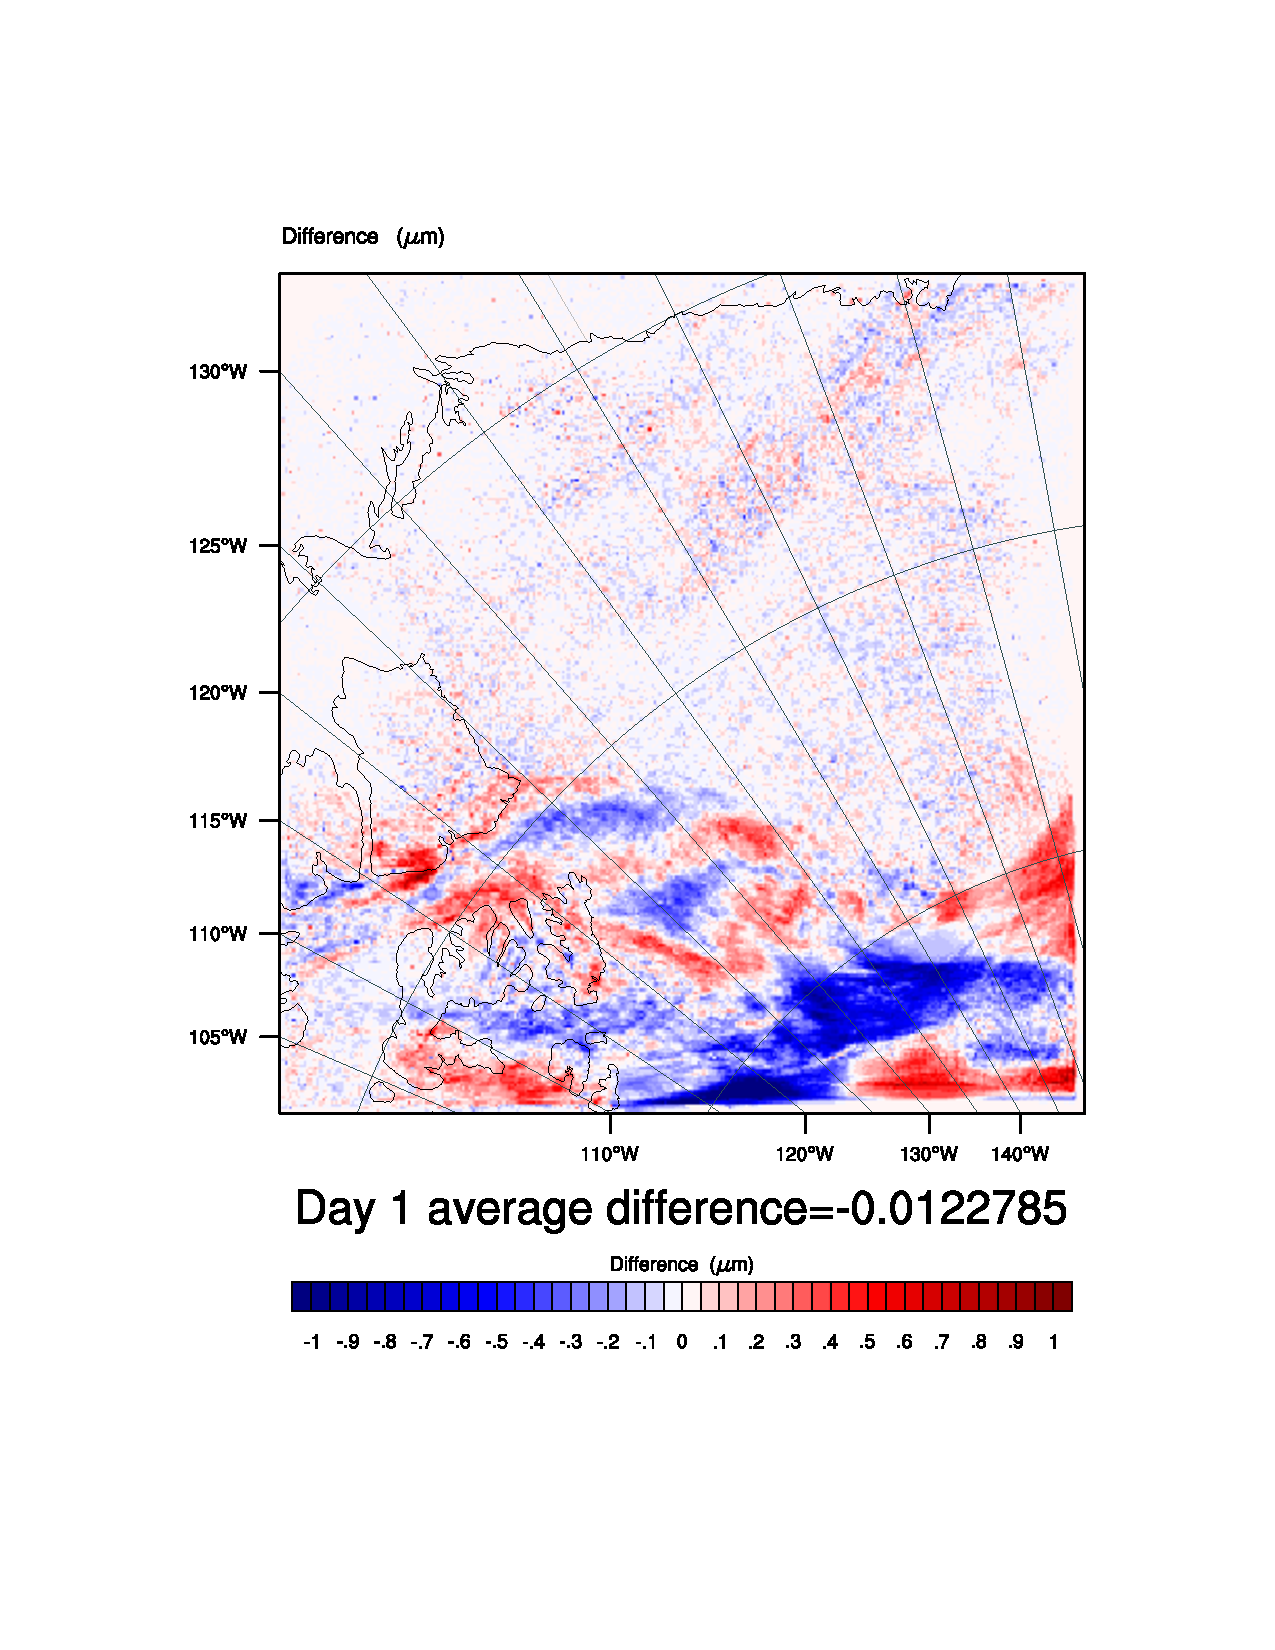
\includegraphics[width=\textwidth]{results/noice/diff_NoIce_RE_CLOUD_Day1.pdf}
		\caption{$r_e$, NoIce, day 1}
		\label{subfig:recloud_r2Day1}
	\end{subfigure}
\caption{The averaged difference in LWP, CDNC and $r_e$ of cloud droplets (from left to right) over the lowermost 11 layers for day 1. NoIce-Control.}
\label{fig:lwpcdncre_r2Day1}
\end{figure}

This implies that there is a new cloud forming in that area, that could not form when there was sea ice. The removal of the sea ice has allowed for increased evaporation and an increase in latent heat (LH) flux which can be seen from figure~\ref{subfig:lh_r2Day1}, where the shape of the area that sea ice was removed from is recognized.

\begin{figure}
\centering
	\begin{subfigure}{0.48\textwidth}
		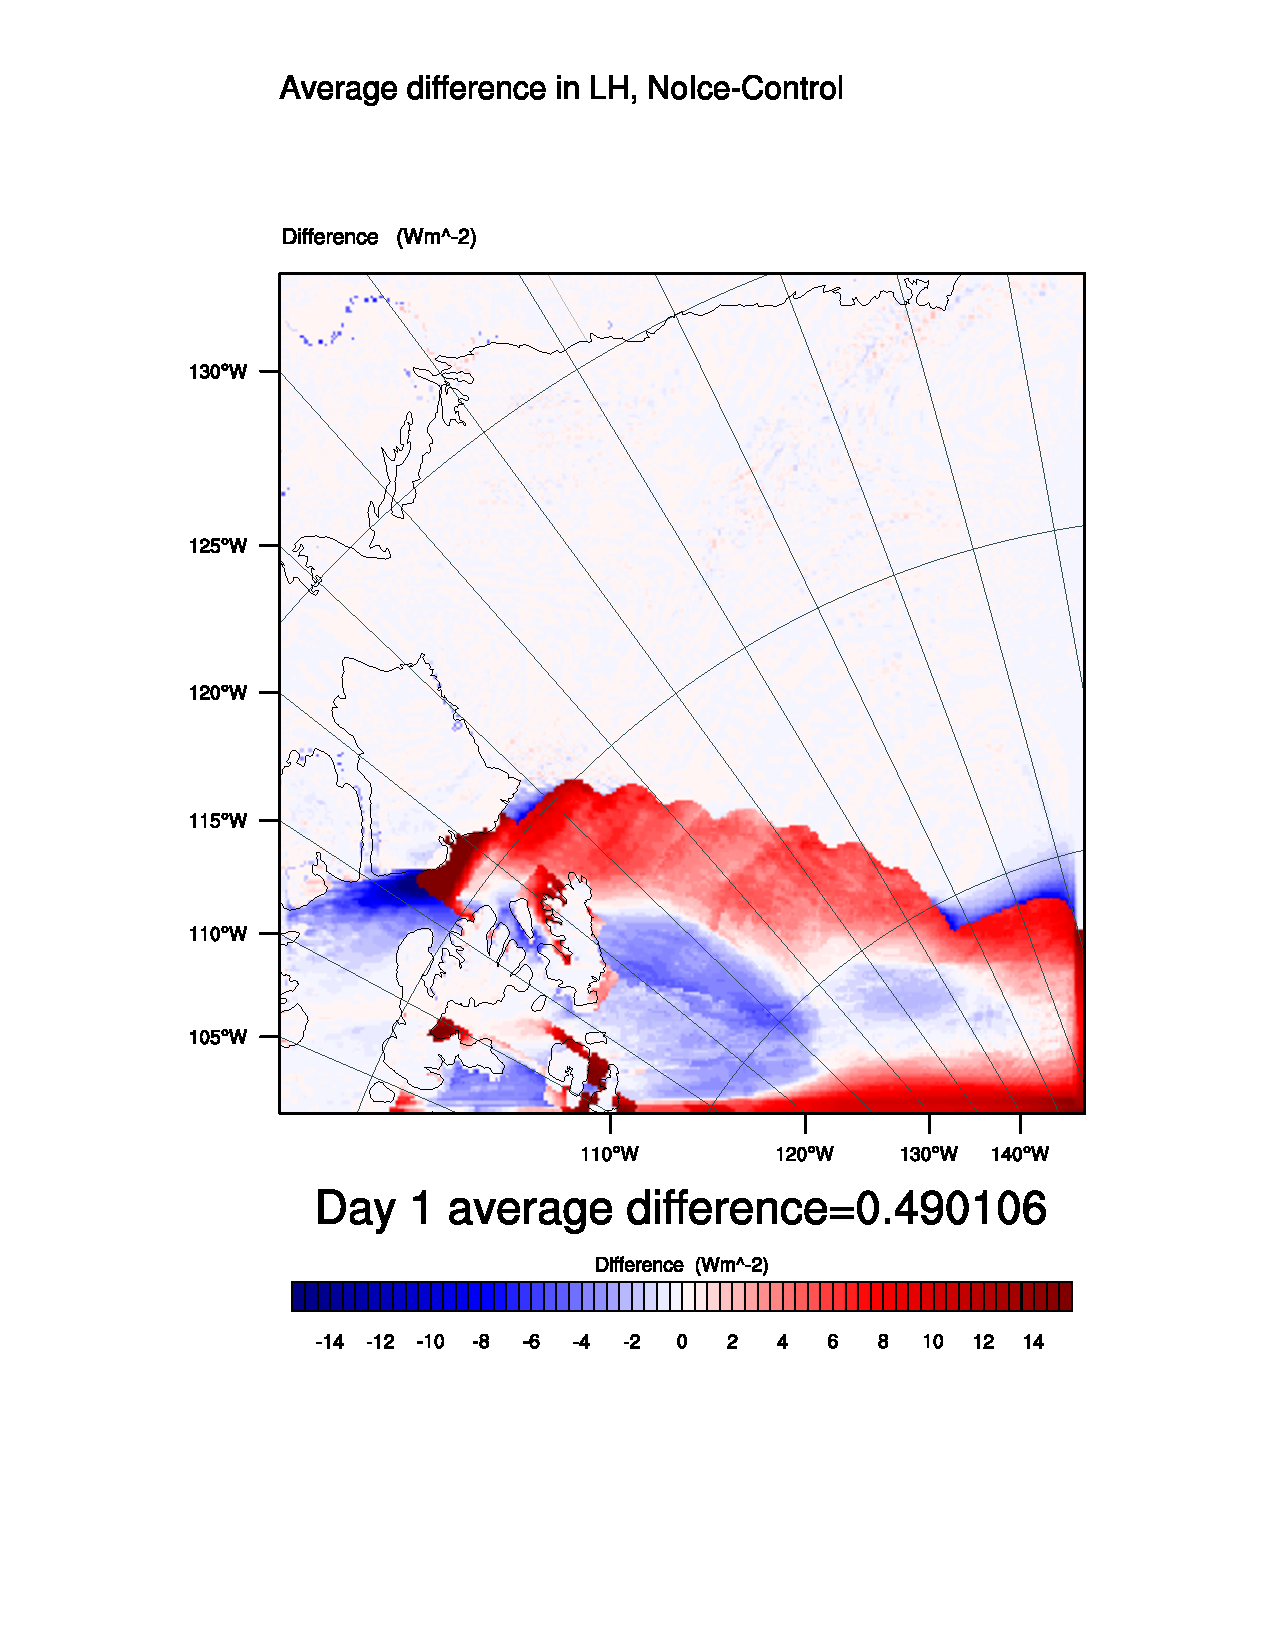
\includegraphics[width=\textwidth]{results/noice/diff_NoIce_LH_Day1.pdf}
		\caption{Difference in LH.}
		\label{subfig:lh_r2Day1}
	\end{subfigure}
	\quad
		\begin{subfigure}{0.48\textwidth}
		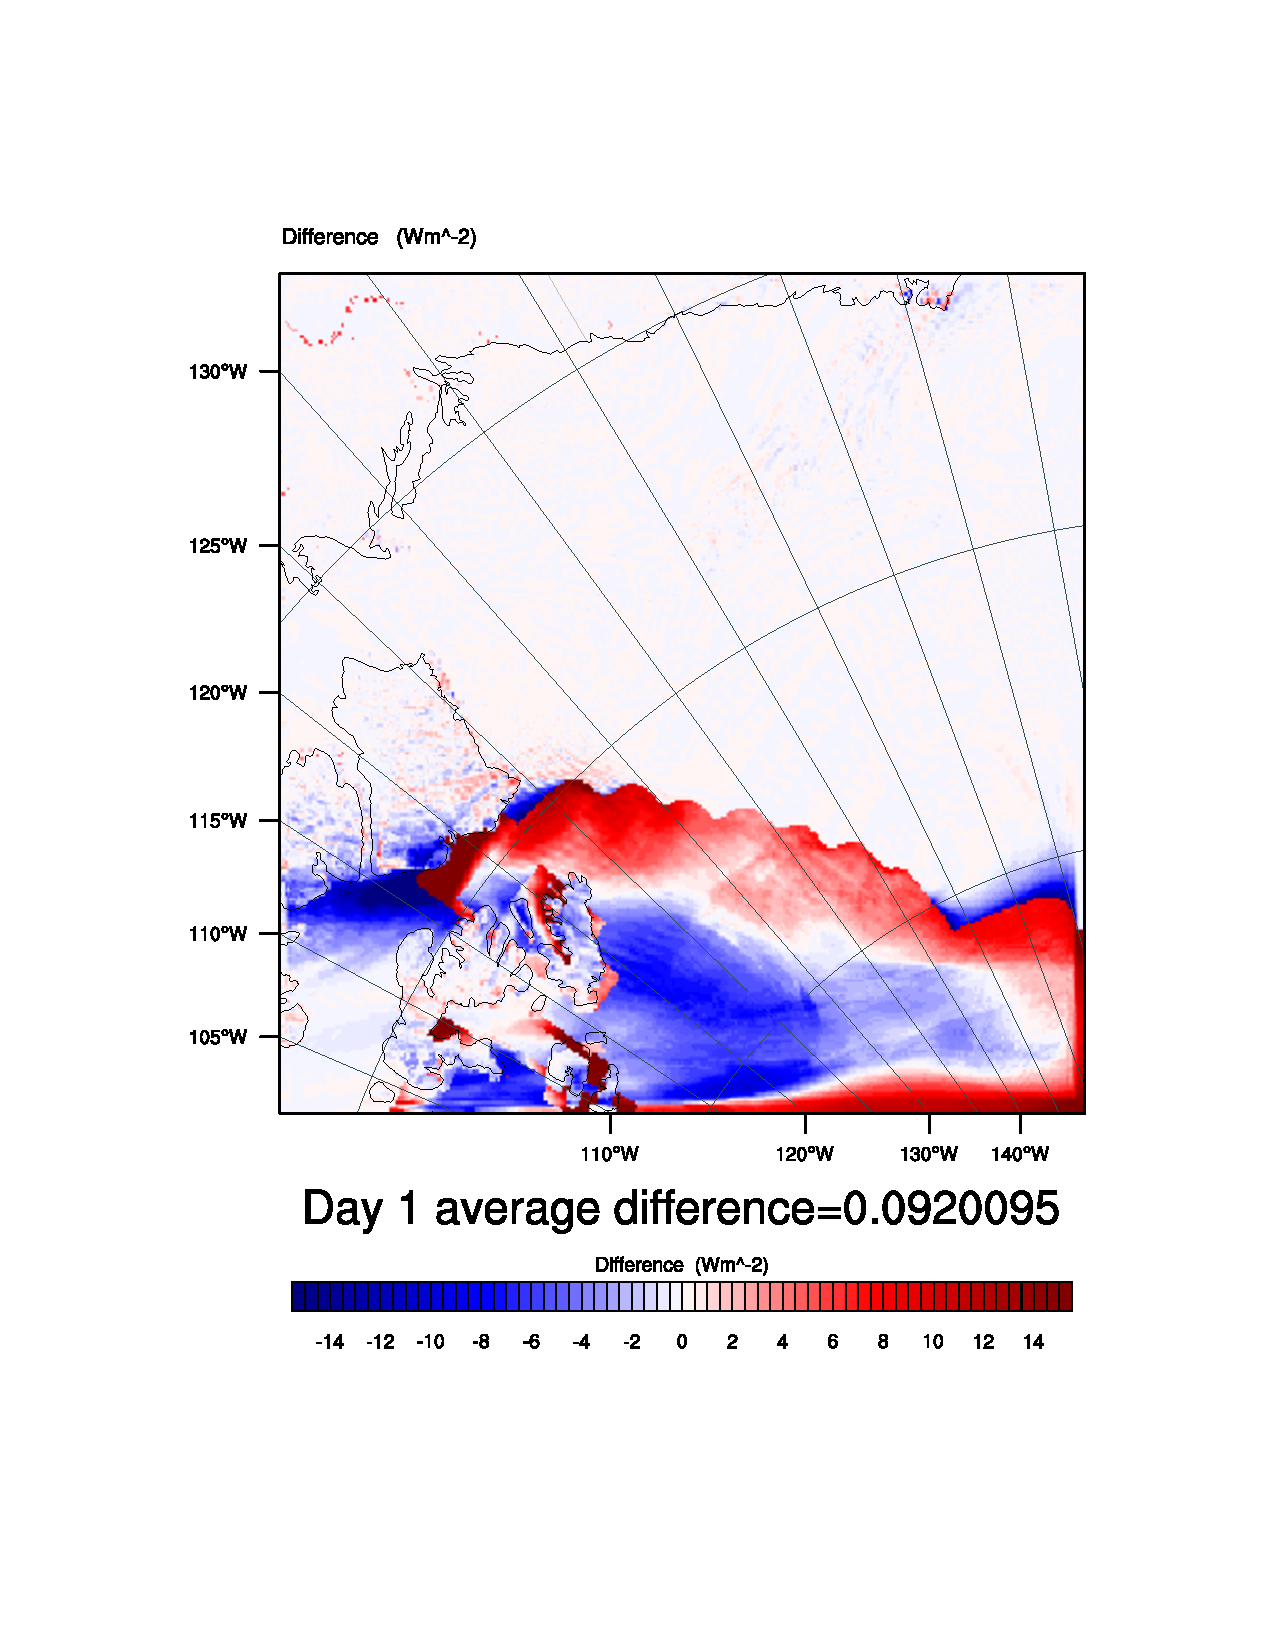
\includegraphics[width=\textwidth]{results/noice/diff_NoIce_HFX_Day1.pdf}
		\caption{Difference in SH.}
		\label{subfig:sh_r2Day1}
	\end{subfigure}
	
		\begin{subfigure}{0.48\textwidth}
		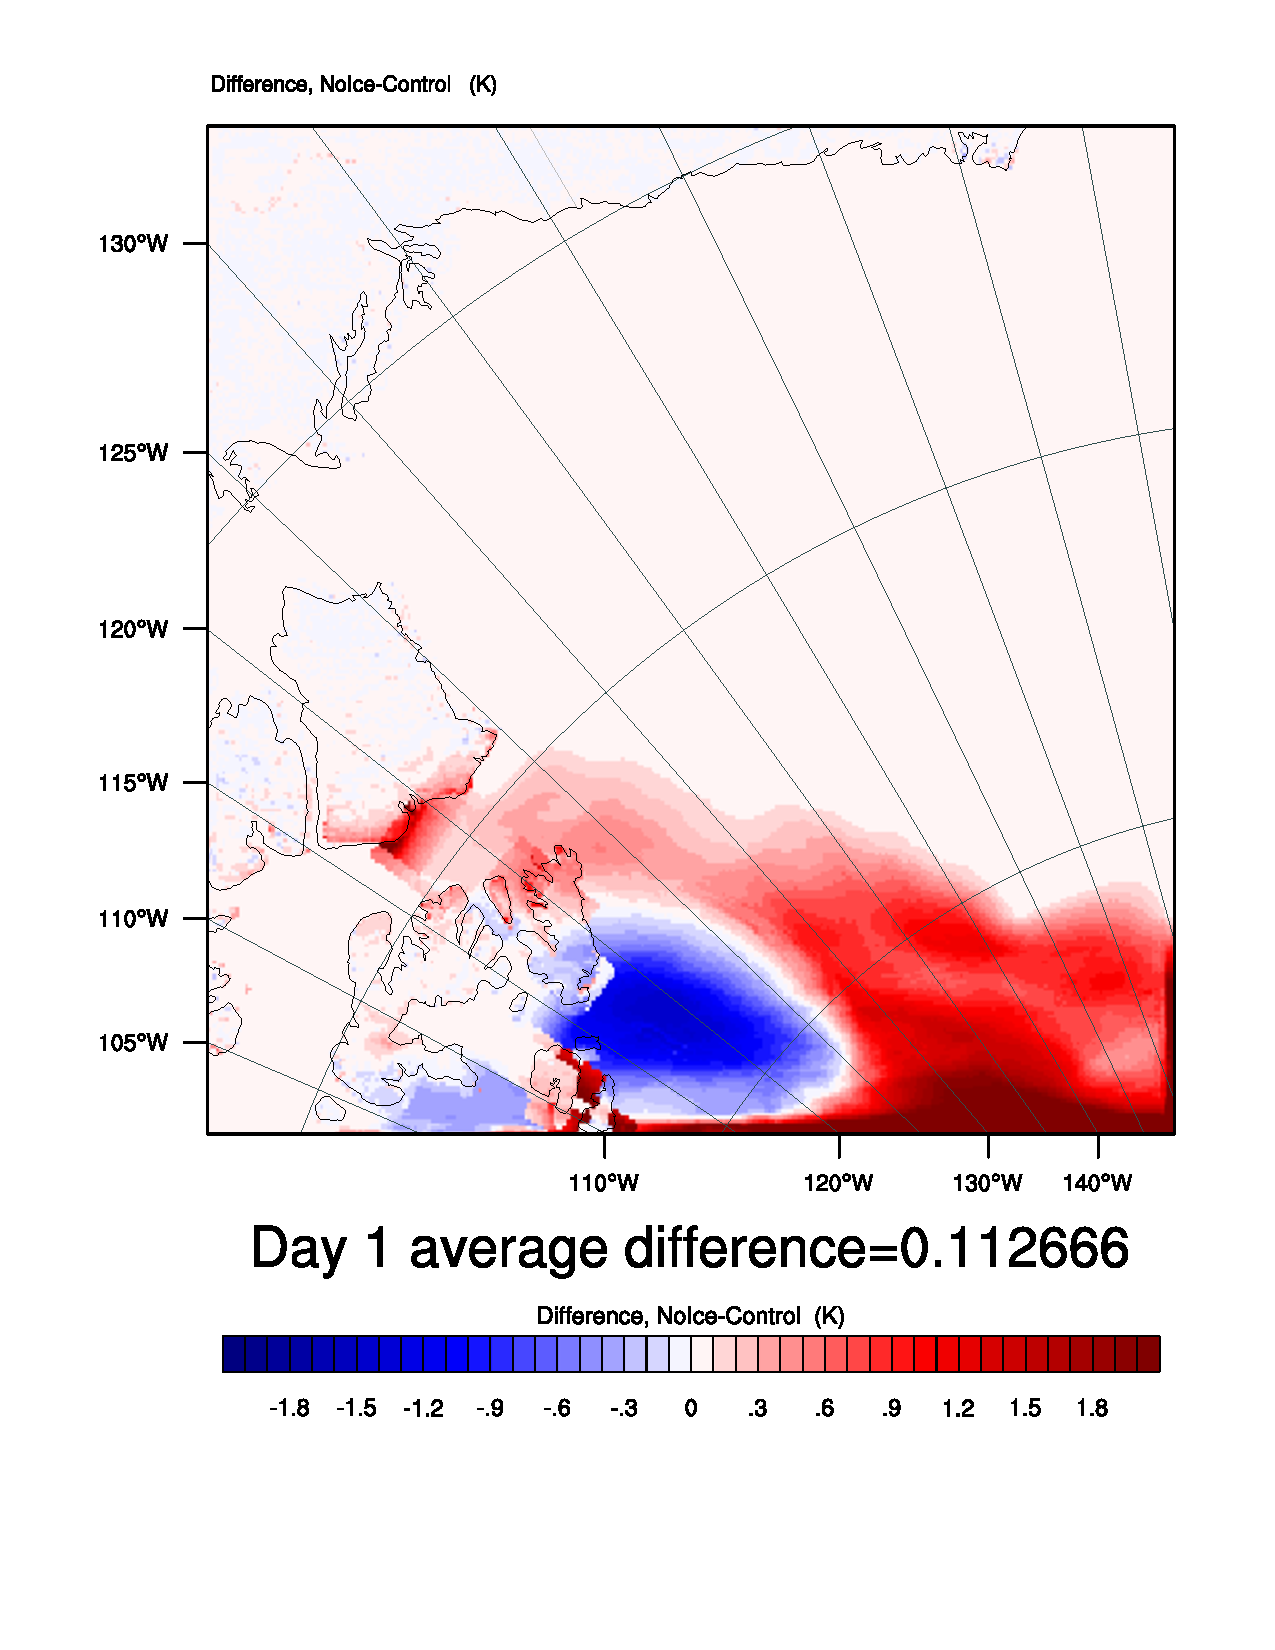
\includegraphics[width=\textwidth]{results/noice/diff_NoIce_skintemp_Day1.pdf}
		\caption{Difference in skin temperature.}
		\label{subfig:skin_r2Day1}
	\end{subfigure}
	\caption{Average difference in LH, SH and skin temperature for day1. NoIce-Control.}
	\label{fig:lhshskin_r2Day1}
\end{figure}

The northernmost part of the study area also has an increase in the cloud droplet number concentration (CDNC), figure~\ref{subfig:CDNCr2Day1}, in the same area as is covered by the red patch indicating an increase in the LWP, which fits well with equation~\ref{eqn:LWC}. There the amount of liquid water is proportional to the droplet number concentration, denoted by $N$ in the equation, and the LWP is the vertically integrated LWC. The average increase in the CDNC would be approximately 1 or 2 droplets per cubic centimeter in the northernmost area. The figure shows the numbers with units $10^6~\text{kg}^{-1}$, which can be approximated to the more common units for CDNC, per cubic centimeter ($\text{cm}^{-3}$). Assuming that the cloud is close enough to the surface to assume a pressure $p=1000~\text{hPa}$, and air density $\rho_a = 1~\text{kg/m}^3=1~\text{kg/}10^6\text{cm}^3$, then for CDNC $10^6/\text{kg} = \text{cm}^{-3}$ is a good approximation. Since CDNC is averaged over 24 hours and 11 layers (to a height of about 1600~m) the CDNC could be higher at certain times, and in certain layers.

The increase in effective radius in the same area as the LWP is increased also indicates the formation of a new cloud,figure~\ref{subfig:recloud_r2Day1}, that could not form in the control run (see figure~\ref{subfig:recloud_r1Day1}).

%The small "blob" at 140$^o$W and about 81$^o$N has decreased $r_e$, most likely because the cloud already was saturated in that area, which can be seen from the LWP from the control run, in figure~\ref{fig:LWPr1Day1}. The possible increase in aerosols from the ocean that would then lead to an increase in CCN would make the water in that cloud spread over more CCN, and by that leave the droplets with a smaller $r_e$.

The the two red patches at 80$\degree$N and 140-155$\degree$W in the figure for difference in $r_e$, figure~\ref{subfig:recloud_r2Day1}, are also clear in the difference in LW downward radiation, figure~\ref{subfig:glw_r2Day1} at the ground surface, and can also be slightly recognized as a decrease in SW downward radiation, figure~\ref{subfig:swdown_r2Day1}. The SW radiation flux at ground surface has been reduced due to the increase in LWP, and the more pronounced decrease in SW is clearly recognized with the same shape and size as the northern patch of increase in LWP. This can be explained by equations~\ref{eqn:cloudalbedo} and~\ref{eqn:cloudtau}, where it is clear from equation~\ref{eqn:cloudtau} that the cloud optical depth, $\tau$, increases with LWP, and following equation~\ref{eqn:cloudalbedo} an increase in $\tau$ would also increase the cloud albedo.

\begin{figure}
\centering
	\begin{subfigure}{0.48\textwidth}
		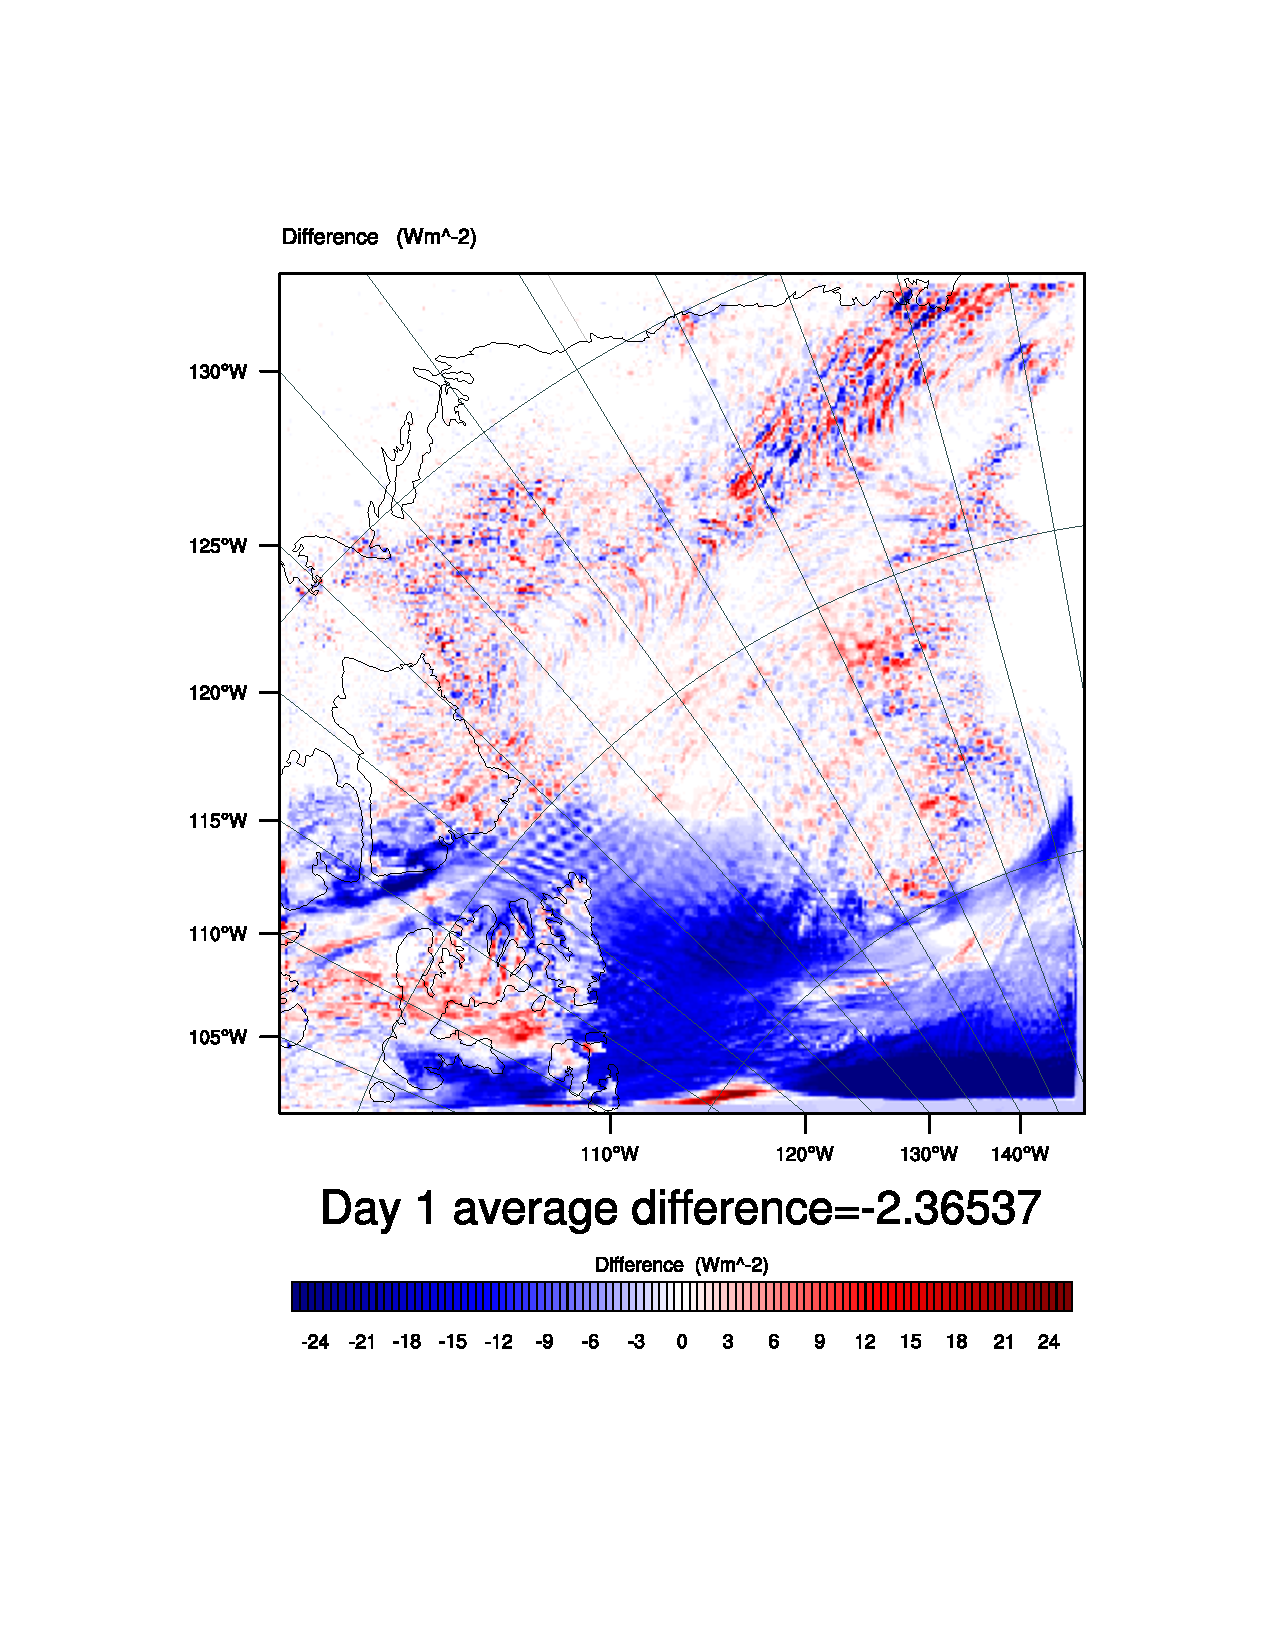
\includegraphics[width=\textwidth]{results/noice/diff_NoIce_SWDOWN_Day1.pdf}
		\caption{The average difference in SW flux down at the surface, day 1.}
		\label{subfig:swdown_r2Day1}
	\end{subfigure}
	\quad
	\begin{subfigure}{0.48\textwidth}
		\centering
		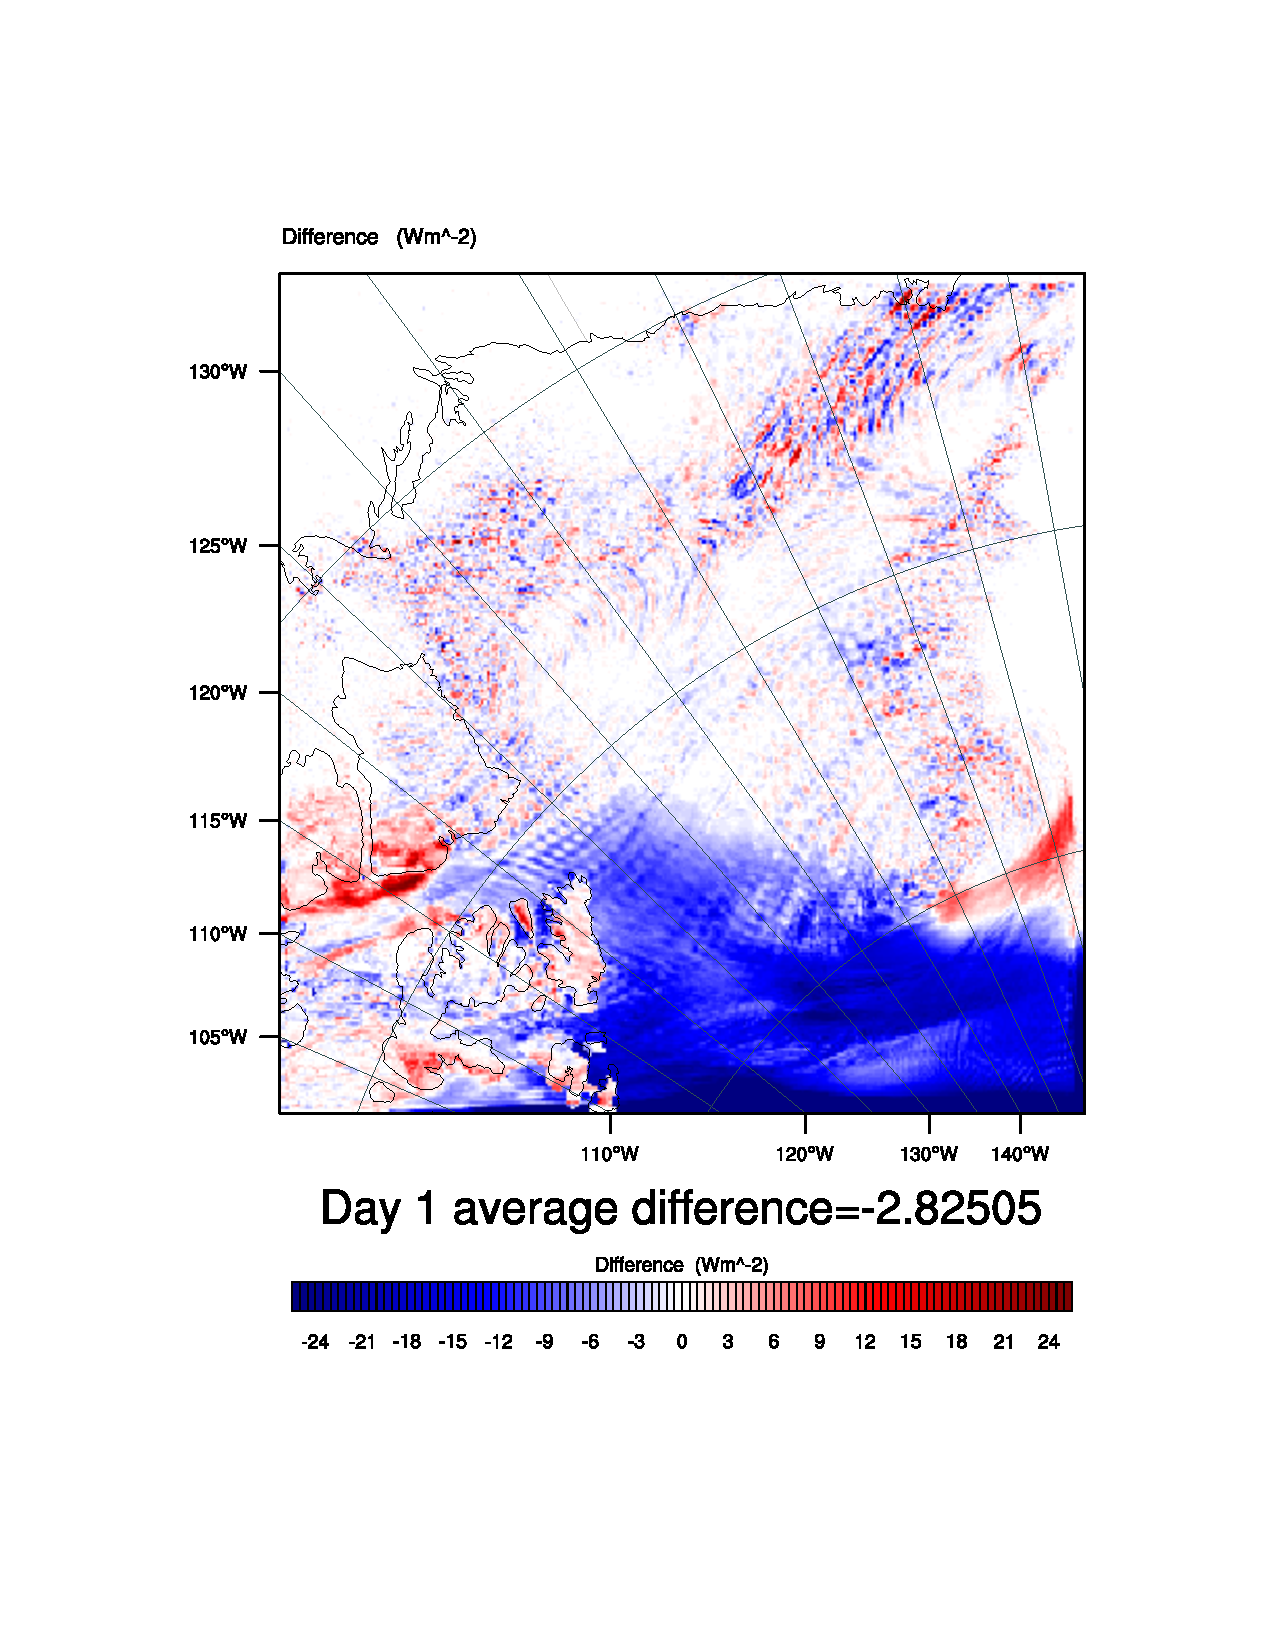
\includegraphics[width=\textwidth]{results/noice/diff_NoIce_SWUPT_Day1.pdf}
		\caption{The average difference in SW flux up at TOA, day 1.}
		\label{subfig:swup_r2Day1}
	\end{subfigure}
	
	\begin{subfigure}{0.48\textwidth}
		\centering
		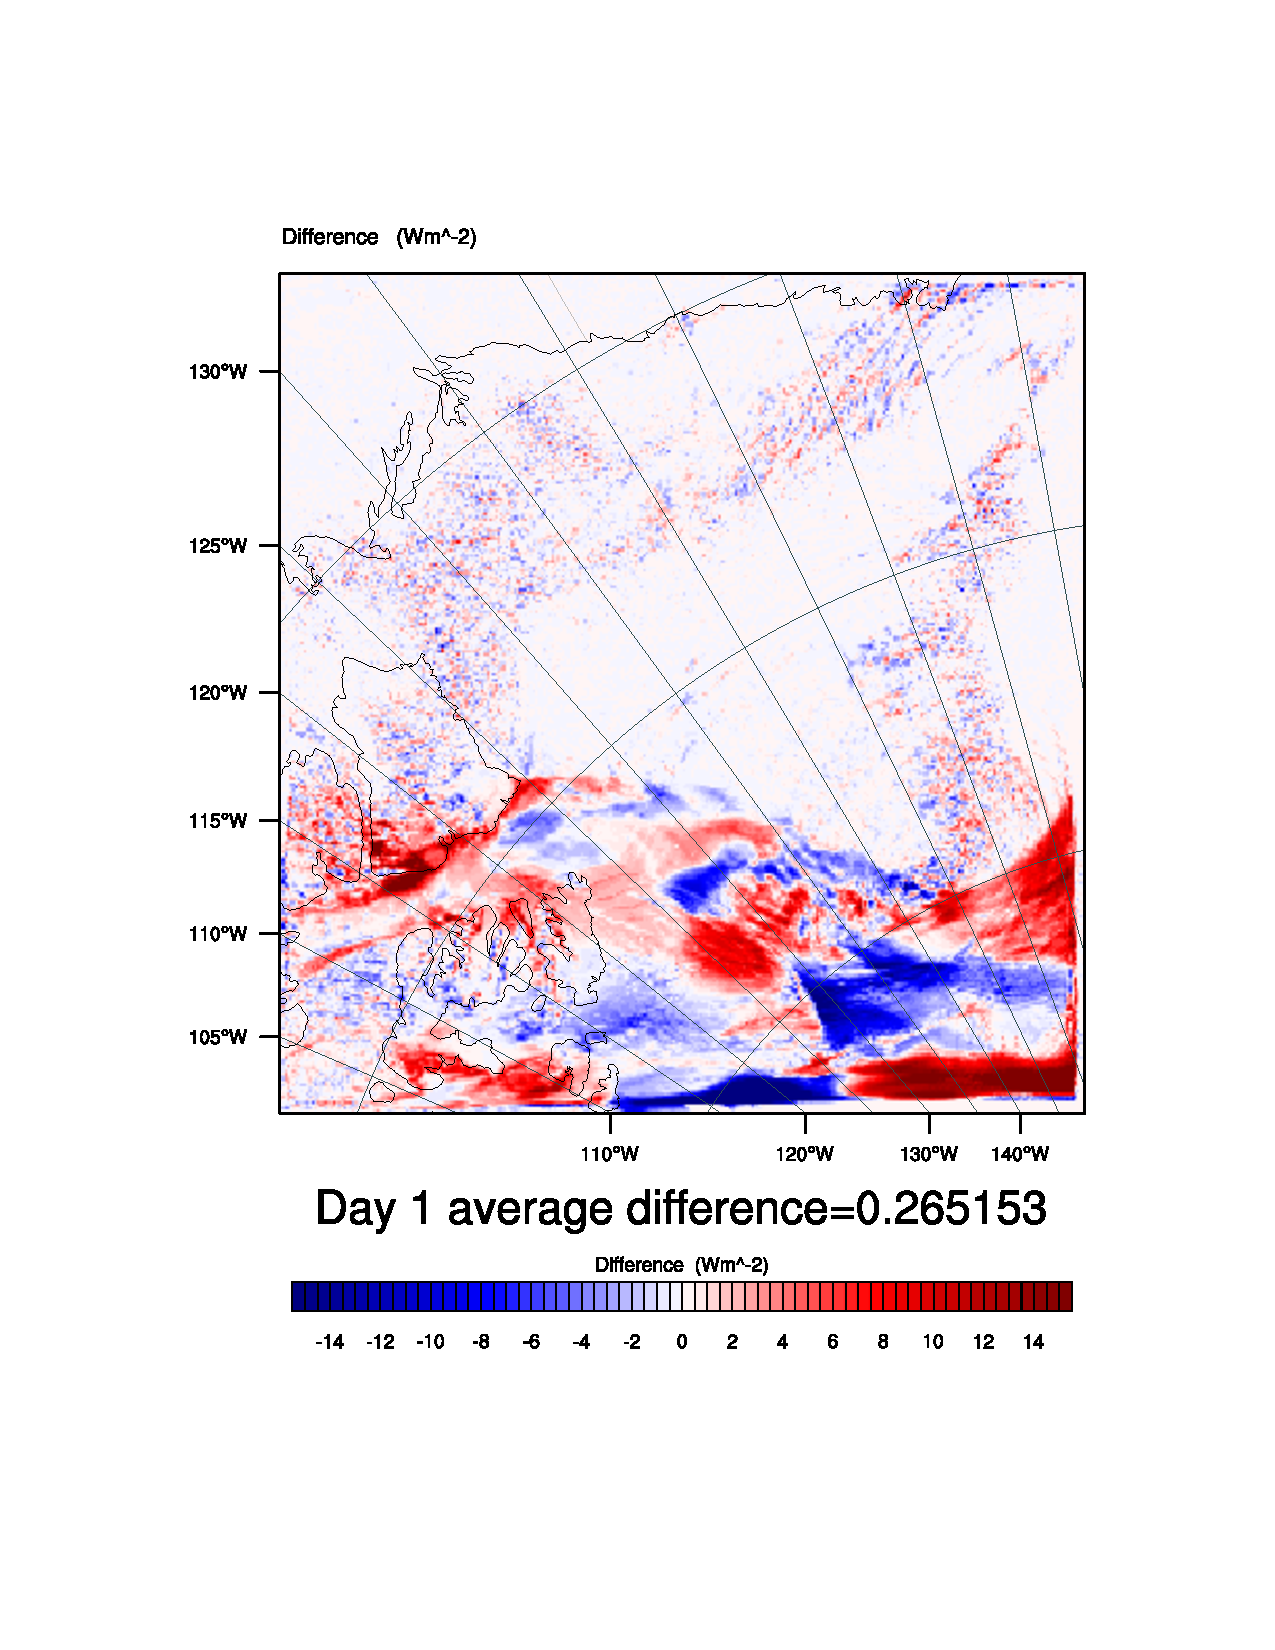
\includegraphics[width=\textwidth]{results/noice/diff_NoIce_GLW_Day1.pdf}
		\caption{The average difference in LW flux down at the surface, day 1.}
		\label{subfig:glw_r2Day1}
	\end{subfigure}
	\quad
	\begin{subfigure}{0.48\textwidth}
		\centering
		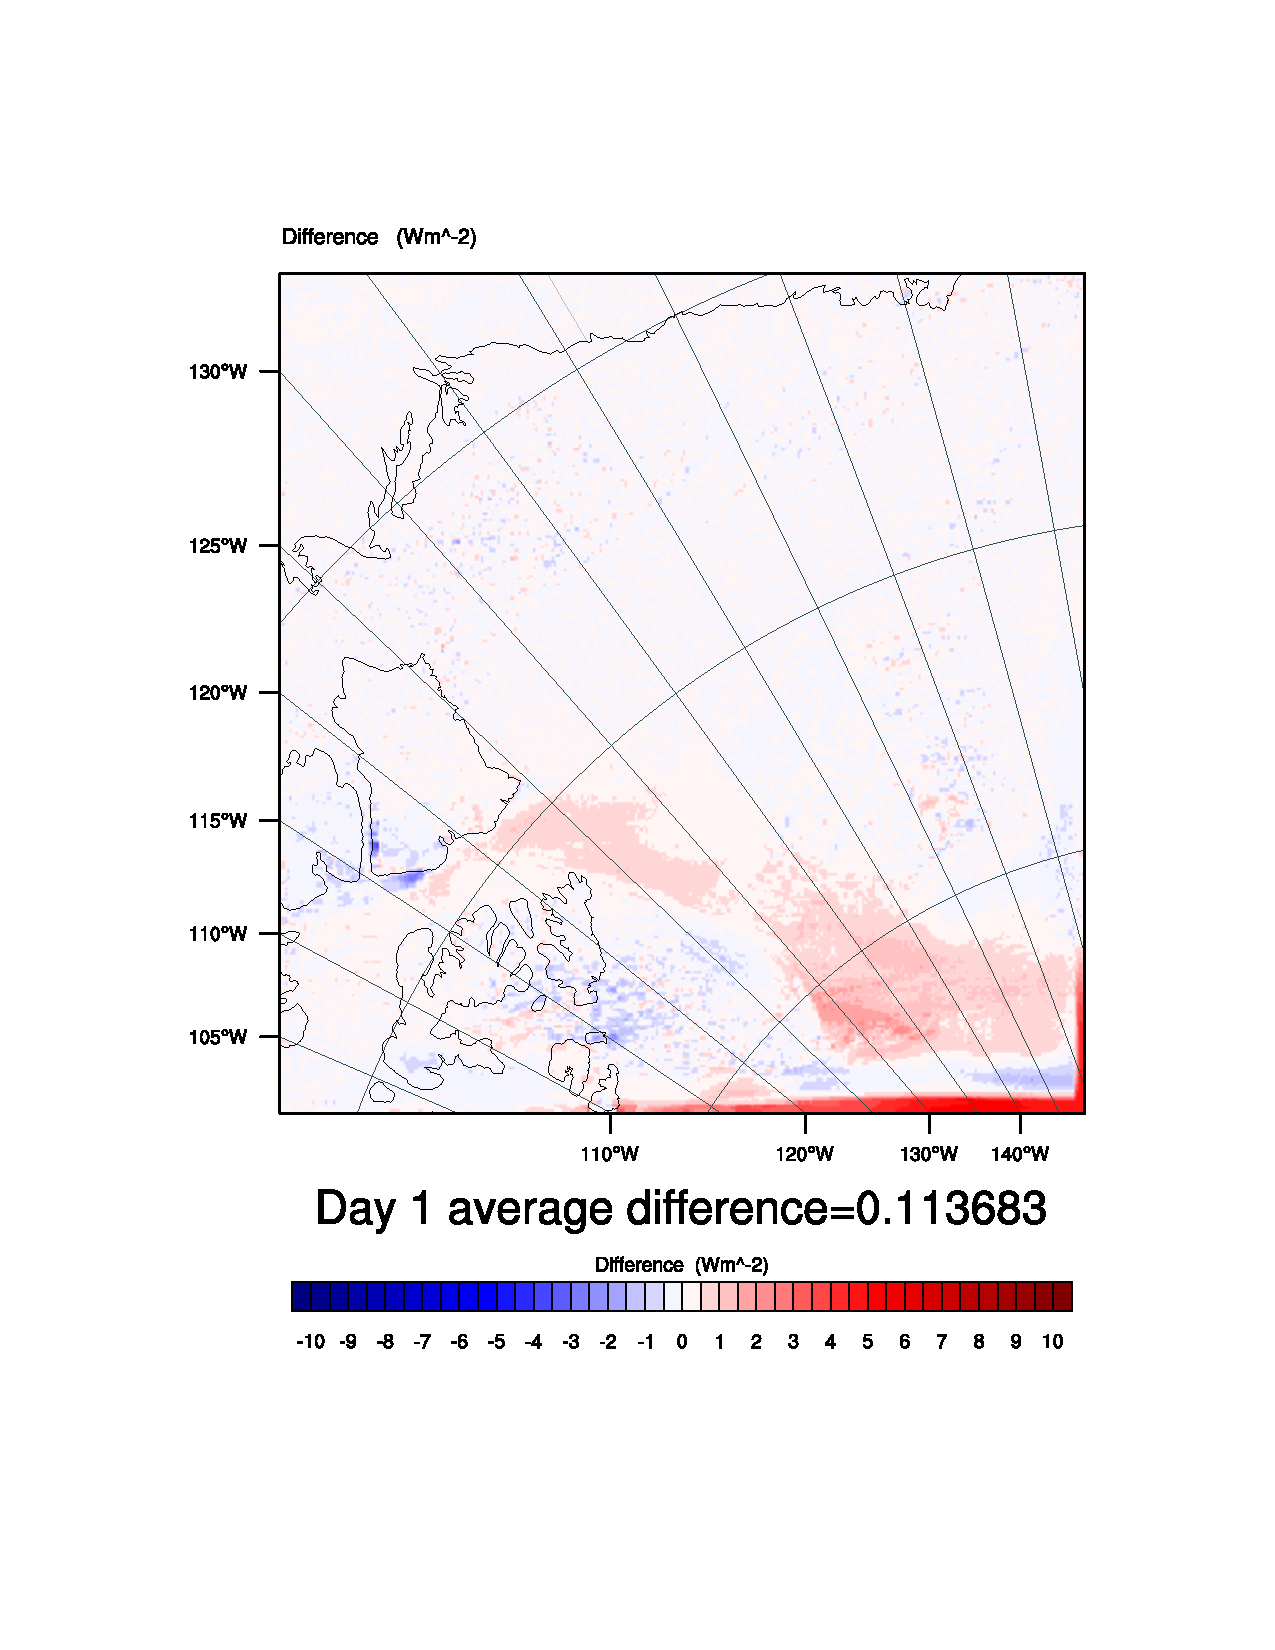
\includegraphics[width=\textwidth]{results/noice/diff_NoIce_LWUPT_Day1.pdf}
		\caption{The average difference in LW flux up at TOA, day 1.}
		\label{subfig:lwup_r2Day1}
	\end{subfigure}
	\caption{The average difference in SW and LW flux down at the surface and up at TOA, for day 1. NoIce-Control.}
	\label{fig:radiation_r2Day1}
\end{figure}

The downward LW radiation flux at the surface (figure~\ref{subfig:glw_r2Day1}) has been increased due to the increase in LWP, which means that there is more water in the clouds and they emit more LW to the ground. It was shown in Chapter~\ref{chap:theory} that an increase in LWP increases the emissivity of the cloud, shown in equation~\ref{eqn:epsilon_lw}, until the cloud is saturated with respect to LW radiation at about 40-45~$\text{g/m}^2$, following figure~\ref{fig:epsalb}.
The slight increase in the LW at TOA is because of increased temperature at the surface when the sea ice is removed (figure~\ref{subfig:skin_r2Day1}).

%The LW at the top of the atmosphere (TOA) does not experience such an increase, in fact it experiences a slight decrease. That it doesn't experience the same increase is explained by the Stefan-Boltzmann's law presented in chapter~\ref{chap:theory}, where the flux density emitted by a body, in this case a cloud, is dependent on the temperature and emissivity of the body (equation~\ref{eqn:stefanboltzmann}).
%The temperature contours in figure~\ref{subfig:cross_LWC_day1}, from the control run, show that the temperature decreases with height and that the clouds hold a lower temperature than there is close to the sea ice. In the run with no ice, the situation is the same (see figure~\ref{subfig:cross_LWC_r2day1}), therefore if clouds with lower temperatures than the surface are the source of the LW reaching TOA the LW reaching TOA would be lower.
%The removal of sea ice has a larger effect on lower clouds than on higher clouds, since the increase in evaporation from the surface doesn't reach high up in the troposphere, especially not in the Arctic, due to the static stability of the lower atmosphere in the Arctic(@cite someone?). Also the LWP showed in this study is only for the lowermost 11 layers and can only explain what happens in those layers, it can not be used as a final explanation for radiation changes that are only at the bottom and top of the modeled atmosphere.
%--------------

Of course, the removal of sea ice would reduce the SW at TOA, see figure~\ref{subfig:swup_r2Day1}. The albedo of sea ice varies between 0.5 and 0.9 depending on snow cover and the age of the ice and is typically 0.5-0.7 for bare ice, whereas a typical ocean albedo is 0.06~\citep{NSIDC}. Thus the change in SW at TOA is negative over the area of ocean where there was sea ice in the control run. The increased SW at TOA at 80$\degree$N and 155$\degree$W is because of the cloud forming in that area, see figure~\ref{subfig:swup_r2Day1}, and can be recognized in the increase in $r_e$ in the same place (figure~\ref{subfig:recloud_r2Day1}) which also represent an increase in LWP and reduction in SW at surface and increase of LW at surface. This is due to the enhanced albedo caused by new clouds at that location, since these figures don't show in-cloud changes, simply the difference between the fields from the run without ice and the control run.

The heat fluxes and surface temperature are almost unchanged for most of the study area by the removal of sea ice, except for the area where the sea ice has been removed (see figures~\ref{subfig:lh_r2Day1},~\ref{subfig:sh_r2Day1} and~\ref{subfig:skin_r2Day1}). For much of the "sea ice removed area" the fluxes are a lot higher than in the control run. This is not surprising, since one would expect the ocean surface to hold a higher temperature than the sea ice, therefore more heat is released than in the case when sea ice is present. This is true except for the blue area at 77-79$\degree$N and 115-125$\degree$W, also from which sea ice has been removed. This indicates a decrease in surface heat fluxes and surface temperature compared with the control run. This area of decrease coincides with that of a decrease in downwelling of both SW and LW at the surface (figures~\ref{subfig:swdown_r2Day1} and~\ref{subfig:glw_r2Day1}). Decreases in downwelling SW and LW radiation could be the reason for the cooling at the surface. It can be seen from figure~\ref{subfig:skin_r2Day1}, that the surface is indeed colder in that area, about 0.9 to 1.5~K colder, than it was in the control run, which is the reason for the decrease in heat fluxes. 

%----------------
\clearpage
\subsection{Day 5}
%----------------
The average differences for LWP, CDNC and $r_e$ at day 5 are all negative, see figure~\ref{fig:lwpcdncre_r2Day5}, over the area that had ice in the control run. Thus the clouds making up the LWP in the control run, see figure~\ref{subfig:LWPr1Day5}, have either ceased to exist, been significantly thinned, moved away or turned into ice. The LWP has a negative difference of >30~$\text{g/m}^2$, which means that the LWP, when comparing with the values for that area in the control run (figure~\ref{subfig:LWPr1Day5}) which were around 40-100~$\text{g/m}^2$, there is still around 20-70$\text{g/m}^2$ left. So the clouds have not all ceased to exist. This is supported by the fact that the CDNC in the control run was $\sim$10 to 25~$\text{cm}^{-3}$ and has according to figure~\ref{subfig:CDNCr2Day5} got 3 to >5 droplets~$\text{cm}^{-3}$ less in the run with no ice. Then the clouds in the run with no ice are left with <5 to around 20 droplets~$\text{cm}^{-3}$ which is definitely enough to assume that there are still clouds in the area.

\begin{figure}[hb]
\centering
	\begin{subfigure}{0.40\textwidth}
		\centering
		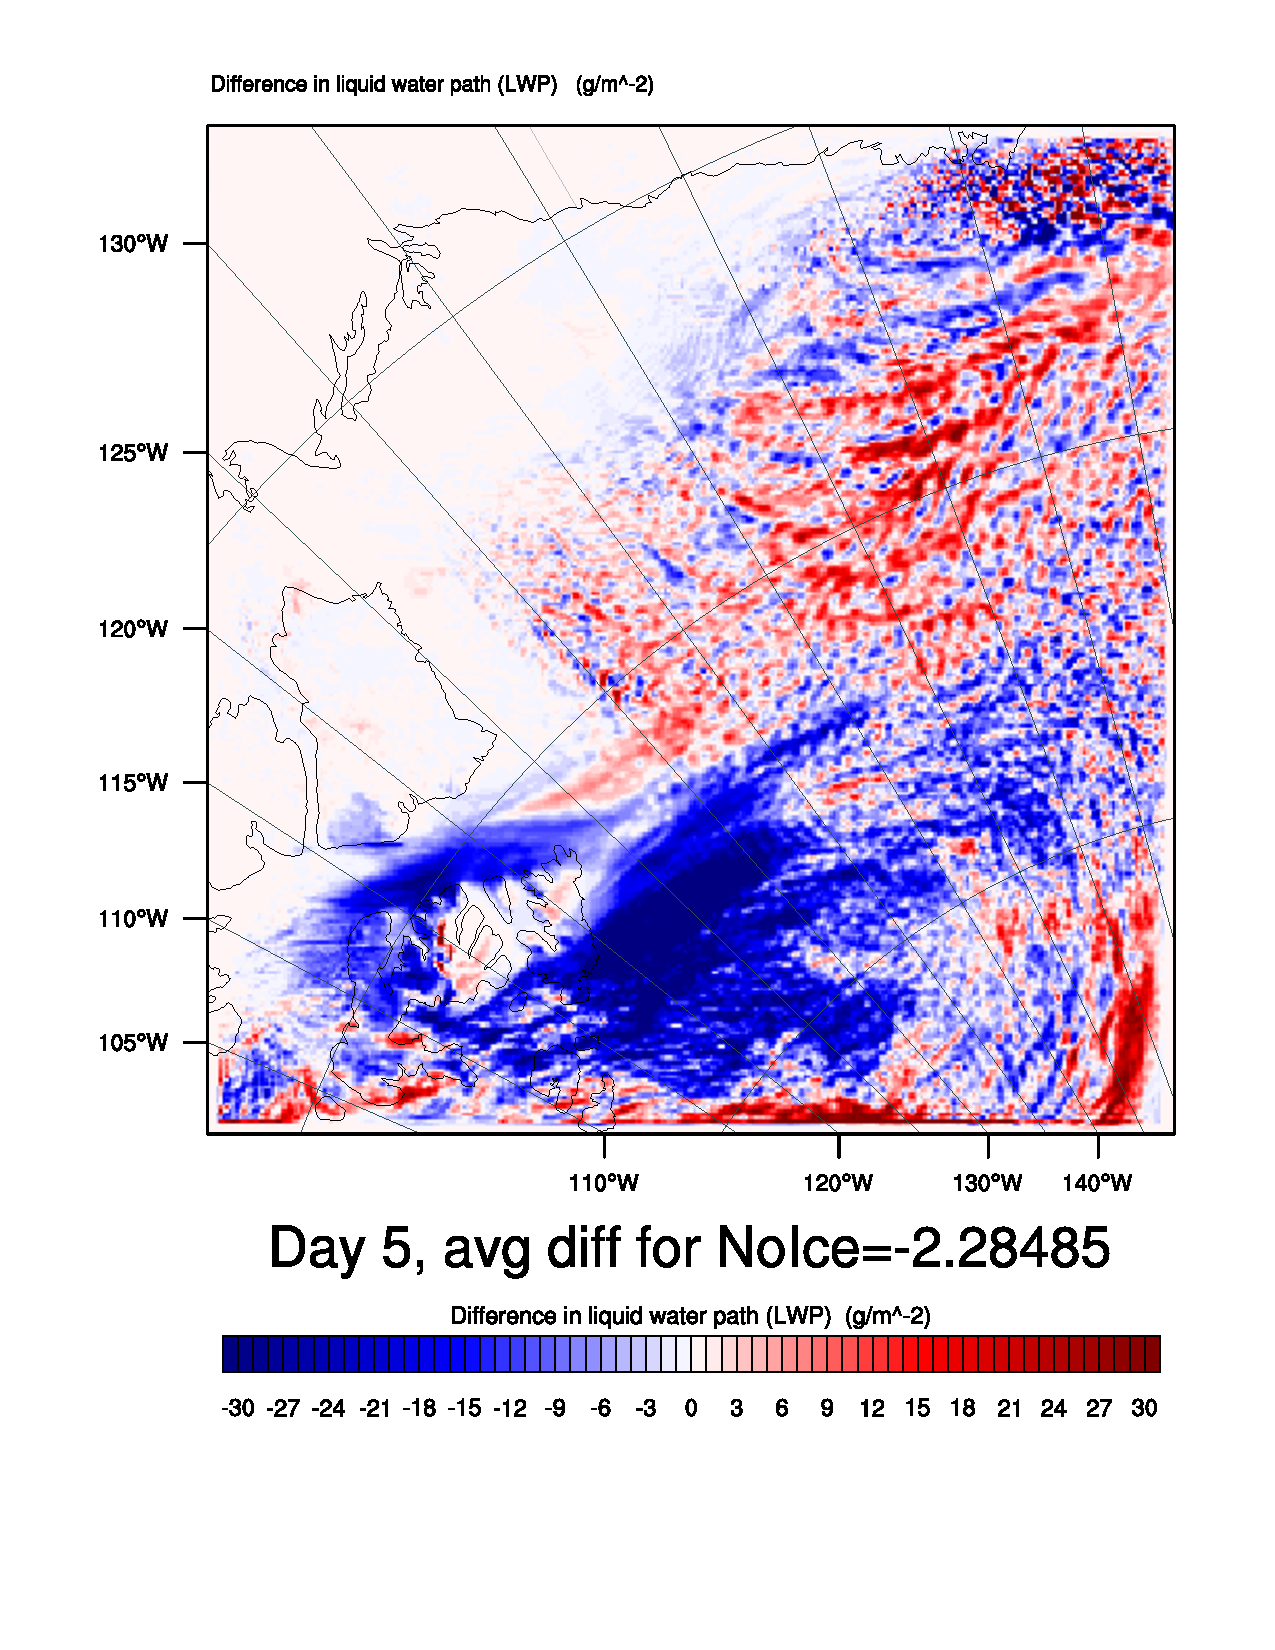
\includegraphics[width=\textwidth]{results/noice/Diff_LWP_Day5NoIce.pdf}
		\caption{LWP, NoIce, day 5}
		\label{subfig:LWPr2Day5}
	\end{subfigure}
	\quad
	\begin{subfigure}{0.40\textwidth}
		\centering
		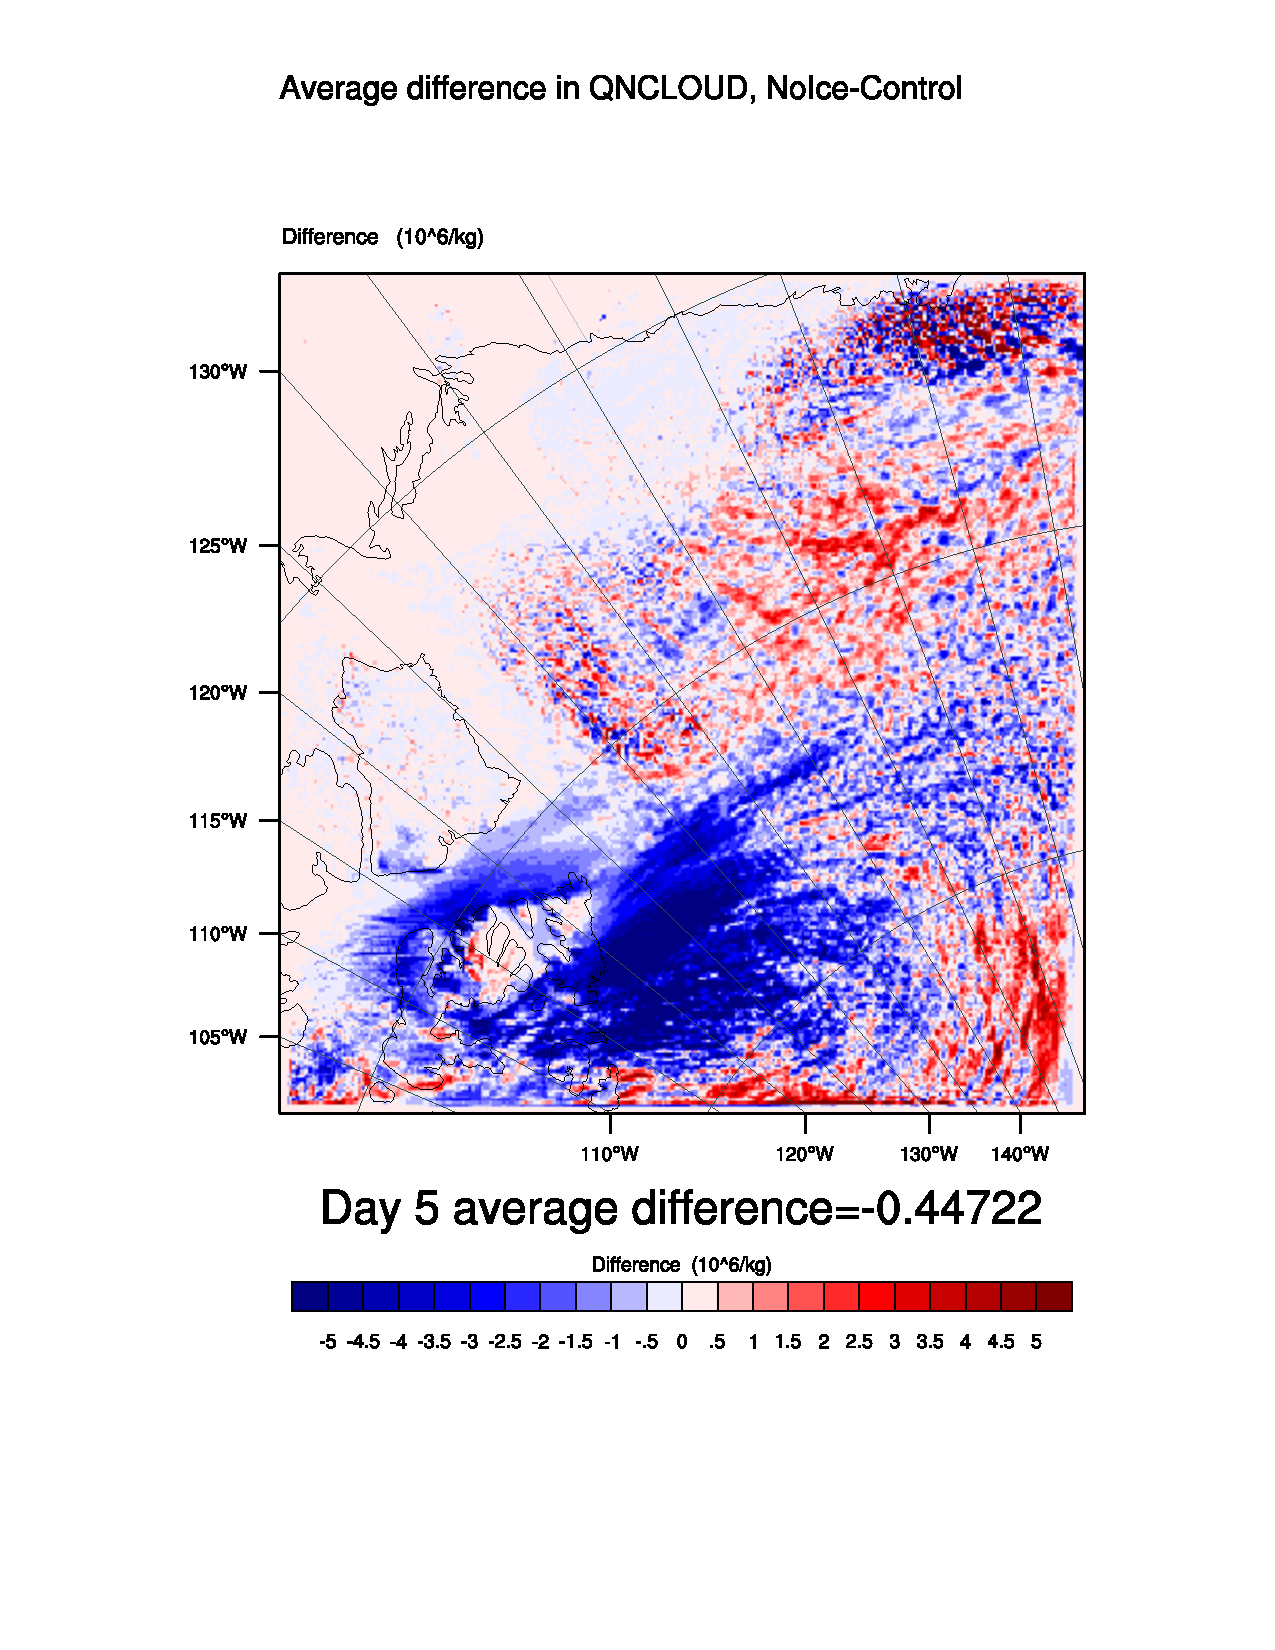
\includegraphics[width=\textwidth]{results/noice/diff_NoIce_QNCLOUD_Day5.pdf}
		\caption{CDNC, NoIce, day 5}
		\label{subfig:CDNCr2Day5}
	\end{subfigure}
	
	\begin{subfigure}{0.40\textwidth}
		\centering
		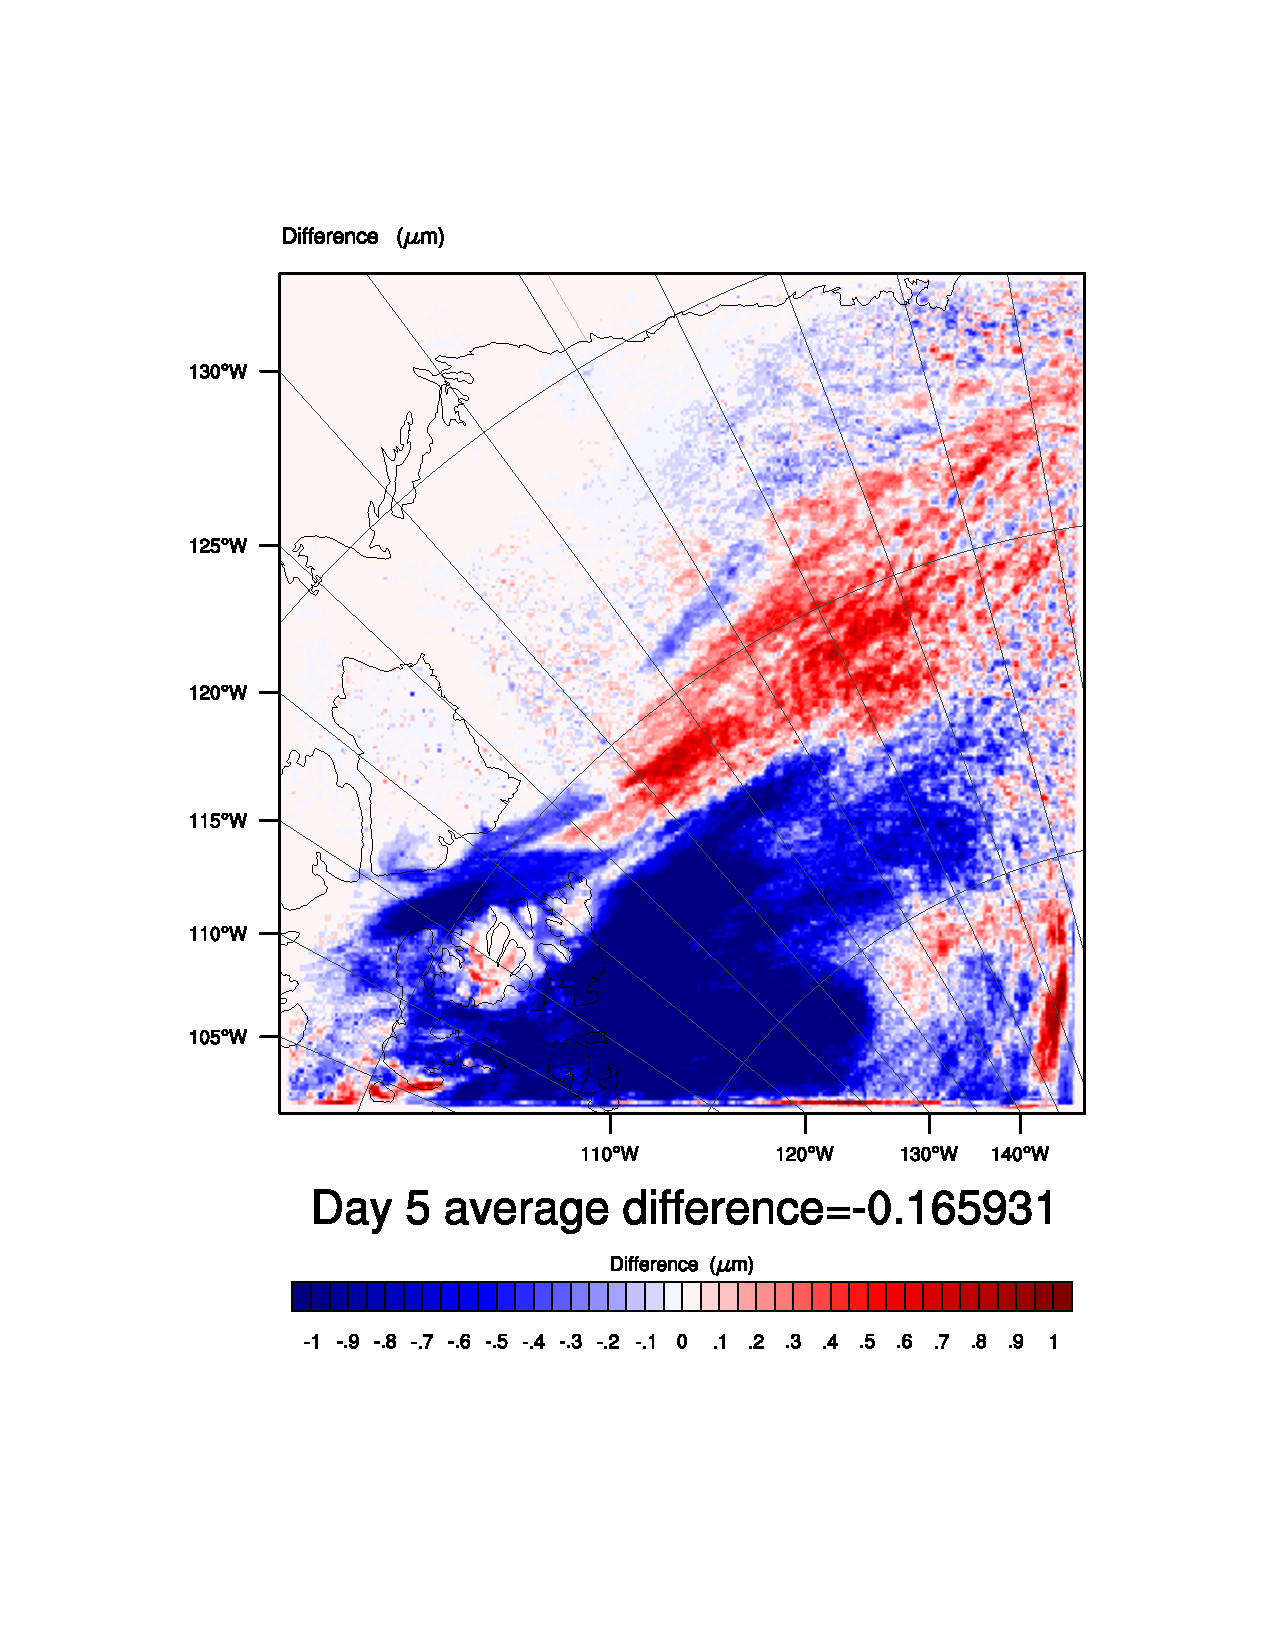
\includegraphics[width=\textwidth]{results/noice/diff_NoIce_RE_CLOUD_Day5.pdf}
		\caption{$r_e$, NoIce, day 5}
		\label{subfig:recloud_r2Day5}
	\end{subfigure}
\caption{The average difference in LWP, CDNC and $r_e$ of cloud droplets (from left to right) over the lowermost 11 layers for day 1. NoIce-Control.}
\label{fig:lwpcdncre_r2Day5}
\end{figure}

There is hardly any ice at all in the study area in the lowermost 11 layers, much like in the control run (see figure~\ref{subfig:cinc_cont_Day5}), and the IWP is zero (not shown) over the area where there was sea ice, and the area around. The wind pattern (not shown) is very much the same as in the control run (figure~\ref{subfig:weather_cont_day5}), and the chance that the clouds have been moved to a different area is ruled out. Therefore precipitation must have depleted the clouds of some of droplets. The difference in rain (not shown) for the run with no ice compared to the control run is negligible and so snow was found guilty of depleting the clouds. Figure~\ref{fig:snowstory} shows how the cloud that was claimed started to form in day 1 of the run with no ice, in section~\ref{sec:noiceDay1}, as more water vapor and aerosols were made available, develops into a snowing cloud and performs natural cloud seeding by snowing out the other clouds as it travels south-east over the sea ice free area.

\begin{figure}
\centering
	\begin{subfigure}{0.32\textwidth}
		\centering
		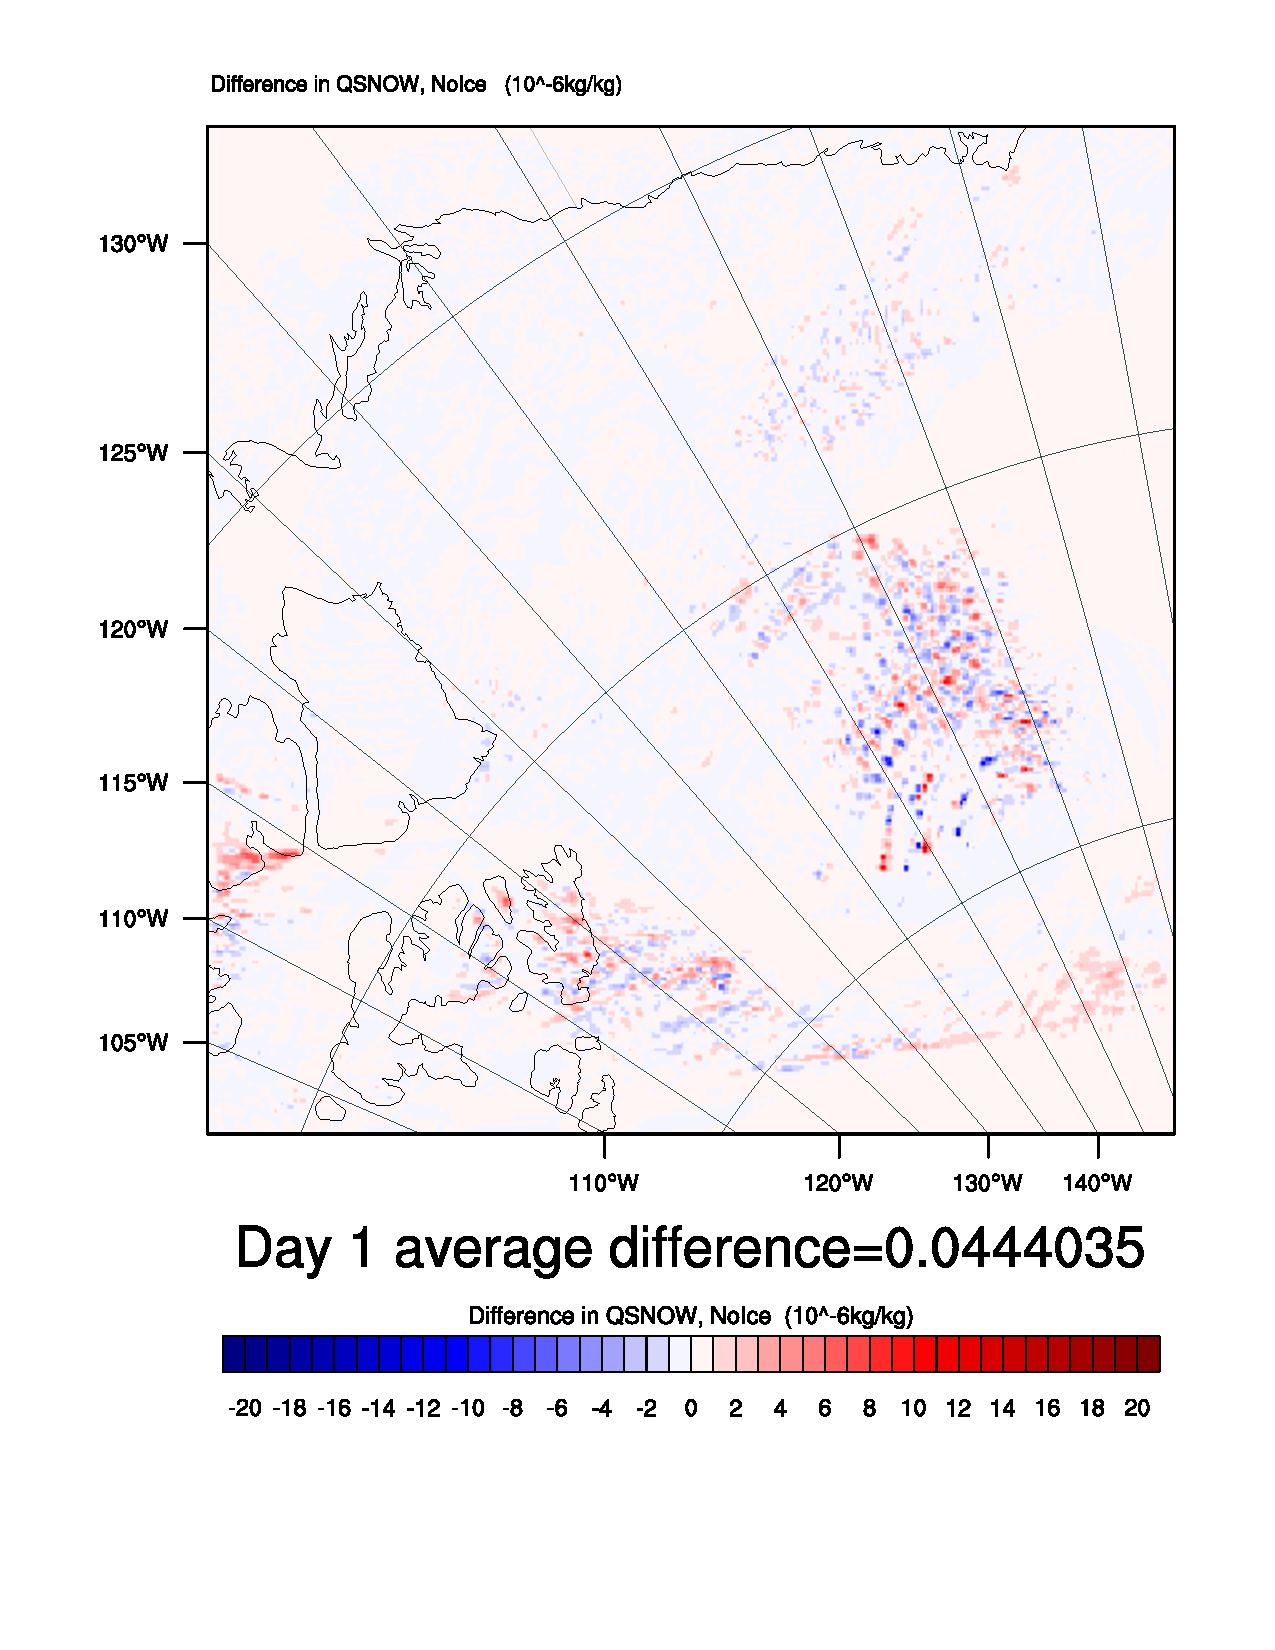
\includegraphics[width=\textwidth]{results/noice/diff_NoIce_qsnow_Day1.pdf}
		\caption{Day 1}
		\label{subfig:snowstory_Day1}
	\end{subfigure}
	\begin{subfigure}{0.32\textwidth}
		\centering
		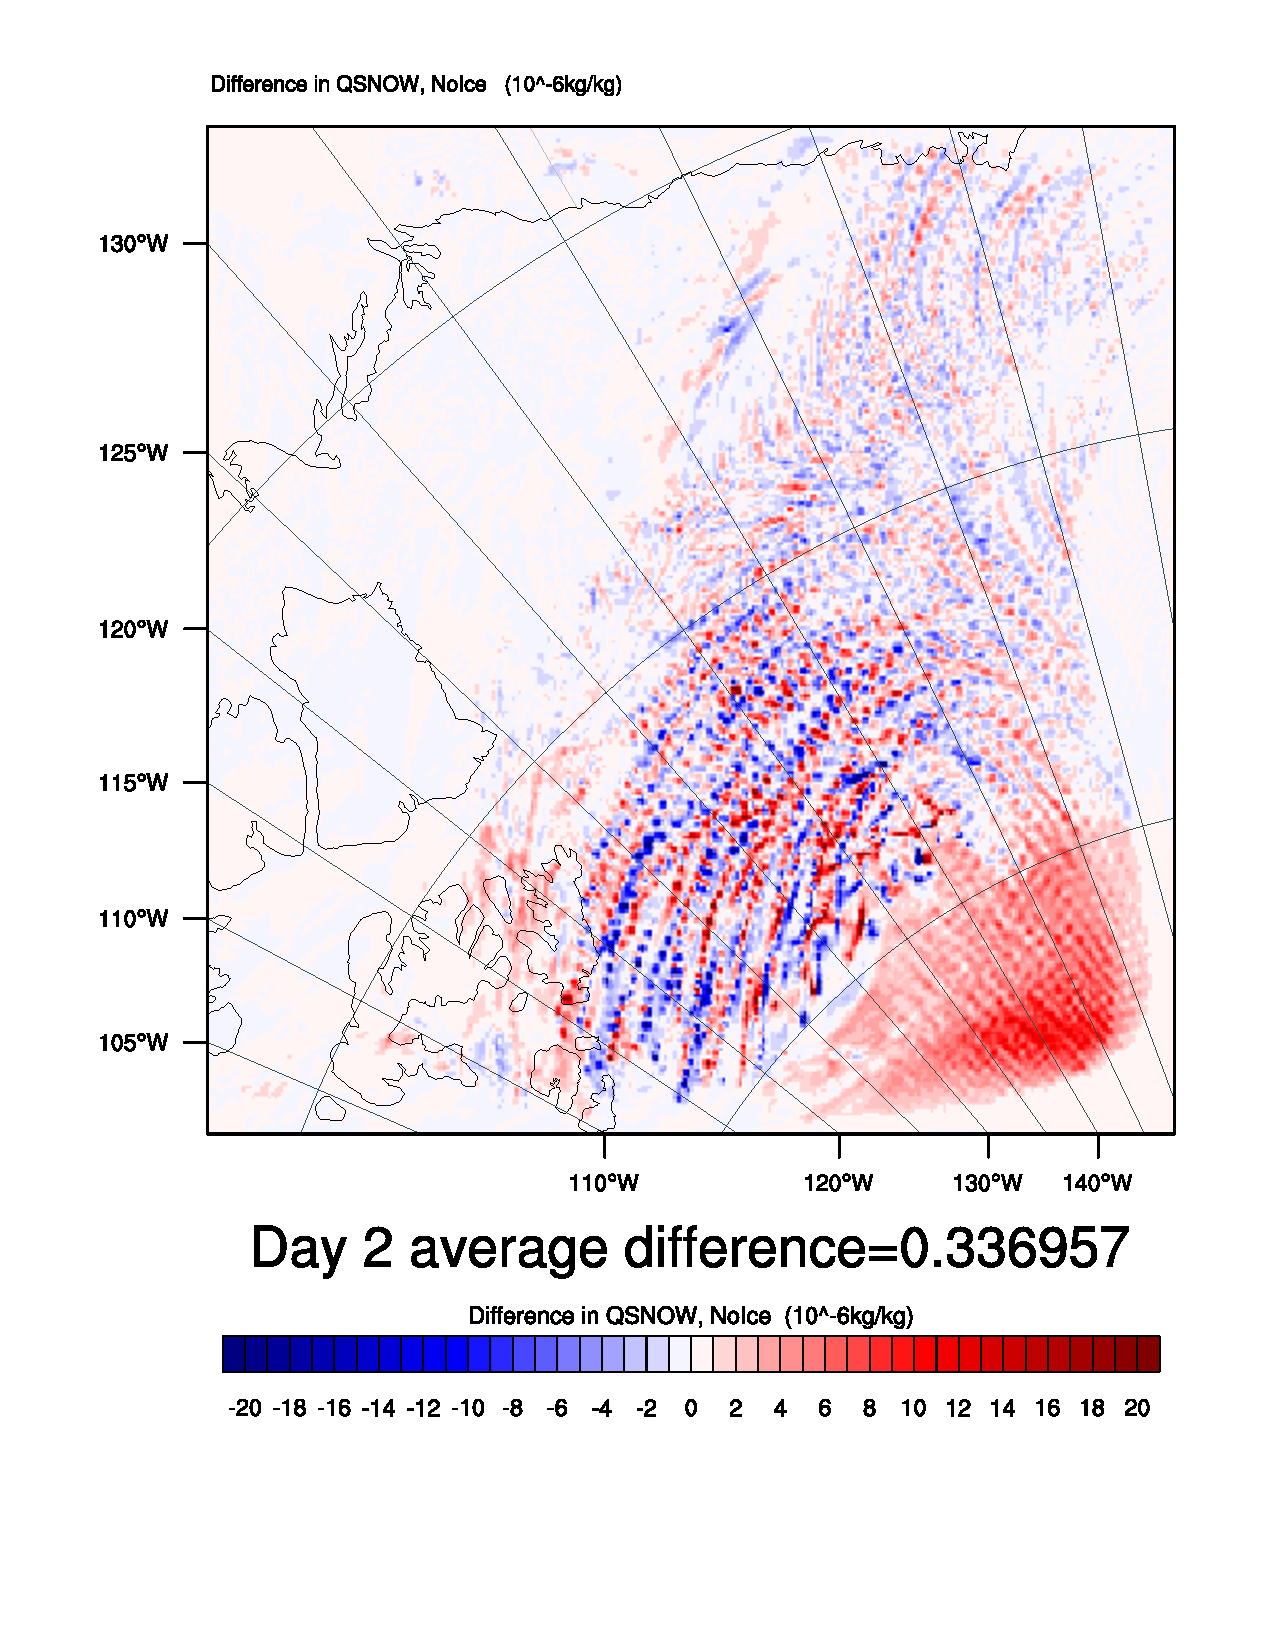
\includegraphics[width=\textwidth]{results/noice/diff_NoIce_qsnow_Day2.pdf}
		\caption{Day 2}
		\label{subfig:snowstory_Day2}
	\end{subfigure}
	\begin{subfigure}{0.32\textwidth}
		\centering
		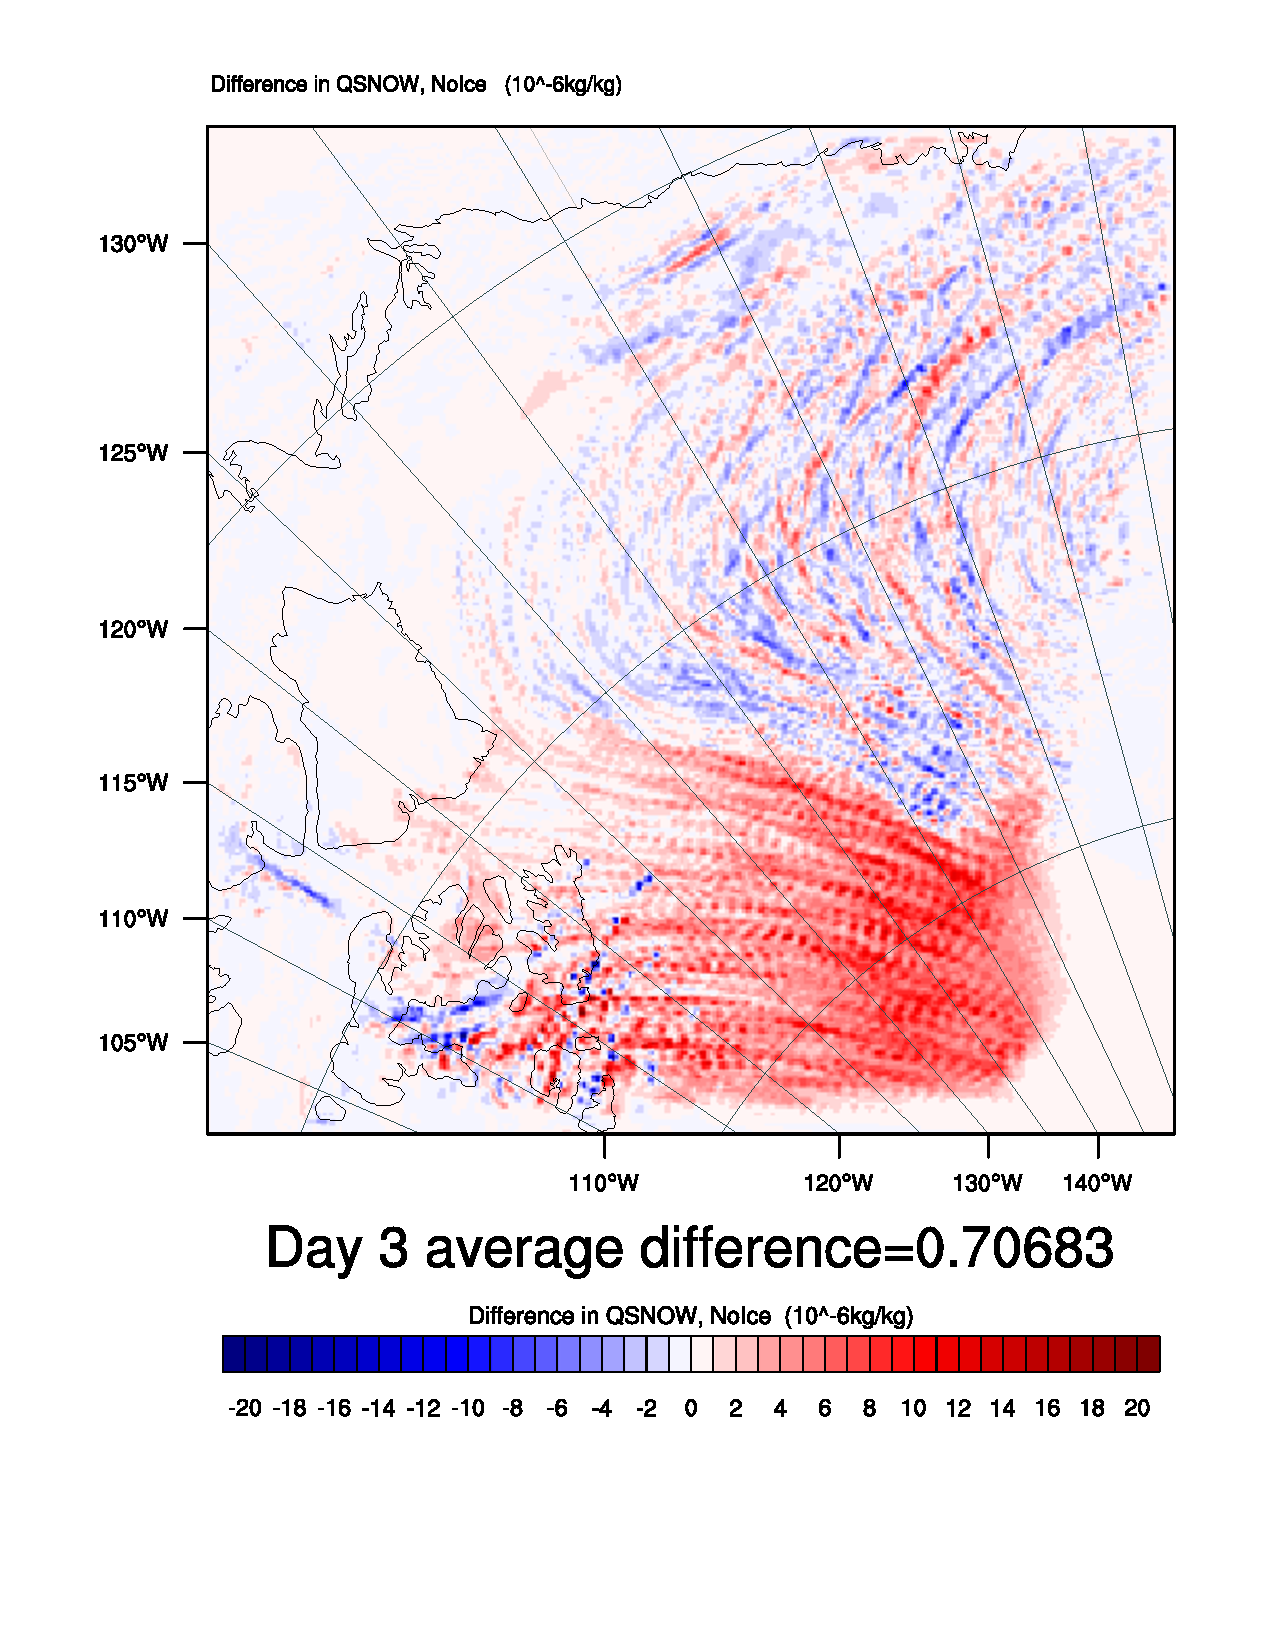
\includegraphics[width=\textwidth]{results/noice/diff_NoIce_qsnow_Day3.pdf}
		\caption{Day 3}
	\end{subfigure}

	\begin{subfigure}{0.32\textwidth}
		\centering
		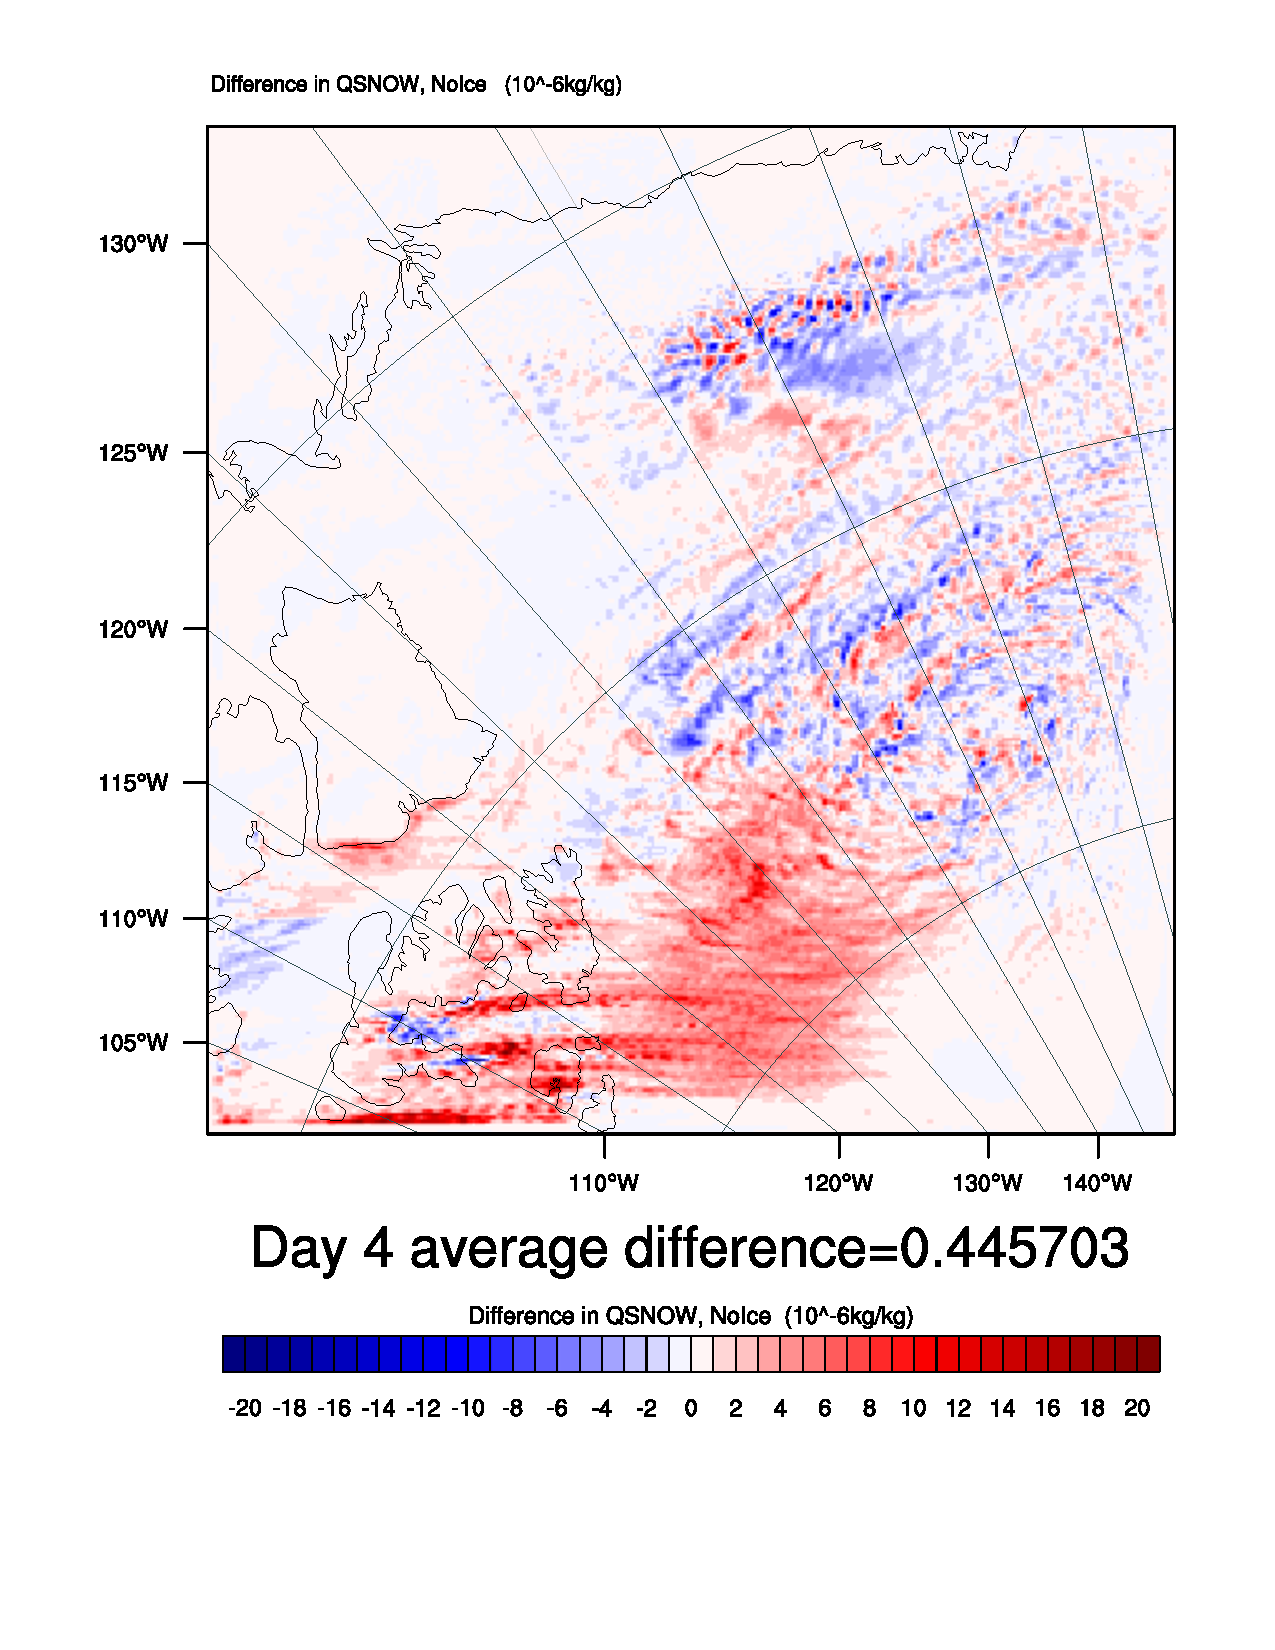
\includegraphics[width=\textwidth]{results/noice/diff_NoIce_qsnow_Day4.pdf}
		\caption{Day 4}
	\end{subfigure}
	\begin{subfigure}{0.32\textwidth}
		\centering
		\includegraphics[width=\textwidth]{results/noice/diff_NoIce_qsnow_Day5.pdf}
		\caption{Day 5}
		\label{subfig:snowstory_Day5}
	\end{subfigure}
\caption{The average difference in mixing ratio of snow to air, over the lowermost 11 layers for days 1 to 5. NoIce-Control.}
\label{fig:snowstory}
\end{figure}

Figure~\ref{subfig:snowstory_Day1} shows the difference in mixing ratio of snow to air averaged for day 1 over the 11 lowermost layers. The slight increase in mixing ratio of snow is in the same area as the red patch in figure~\ref{subfig:CDNCr2Day5} that was claimed to be a forming cloud. Figure~\ref{subfig:snowstory_Day2} shows that in day 2 the cloud has indeed formed and it starts its journey south-eastward and continues through to day 5, see figure~\ref{subfig:snowstory_Day5} where the positive difference in snow is less pronounced, but still present.

The clouds on the 5th day of the run with no ice are now significantly thinner than the clouds in the 5th day of the control run, due to the aforementioned reduction in CDNC. This allows for more of the upwelling LW at TOA to come directly from the surface, which holds a higher temperature than the atmosphere above (see cross section in figure~\ref{subfig:cross_LWC_Day5}) and the newly ice free area also has a higher skin temperature, an increase of $\sim$1$\degree$C than the area did in the control run, when there was sea ice there (see figure~\ref{subfig:skin_r2Day5}). Following Stefan-Boltzmann's law (equation~\ref{eqn:stefanboltzmann}) the surface should now emit more LW than the clouds and sea ice with lower temperatures in the control run did. Figure~\ref{subfig:lwup_r2Day5} shows that the upwelling LW at TOA has indeed increased by $\sim$0.5 to 5 $\text{W/m}^2$ over the area where sea ice has been removed. Overall the average increase in upwelling LW at TOA for the whole area is just shy of 0.5, but the area of particular interest is where the sea ice has been removed, and that shows a more pronounced difference than the rest of the field.

\begin{figure}
\centering
	\begin{subfigure}{0.48\textwidth}
		\includegraphics[width=\textwidth]{results/noice/diff_NoIce_SWDOWN_Day5.pdf}
		\caption{The average difference in SW flux down at the surface, day 5.}
		\label{subfig:swdown_r2Day5}
	\end{subfigure}
	\quad
	\begin{subfigure}{0.48\textwidth}
		\centering
		\includegraphics[width=\textwidth]{results/noice/diff_NoIce_SWUPT_Day5.pdf}
		\caption{The average difference in SW flux up at TOA, day 5.}
		\label{subfig:swup_r2Day5}
	\end{subfigure}
	
	\begin{subfigure}{0.48\textwidth}
		\centering
		\includegraphics[width=\textwidth]{results/noice/diff_NoIce_GLW_Day5.pdf}
		\caption{The average difference in LW flux down at the surface, day 5.}
		\label{subfig:glw_r2Day5}
	\end{subfigure}
	\quad
	\begin{subfigure}{0.48\textwidth}
		\centering
		\includegraphics[width=\textwidth]{results/noice/diff_NoIce_LWUPT_Day5.pdf}
		\caption{The average difference in LW flux up at TOA, day 5.}
		\label{subfig:lwup_r2Day5}
	\end{subfigure}
	\caption{The average difference in SW and LW flux down at the surface and up at TOA, for day 5. NoIce-Control.}
	\label{fig:radiation_r2Day5}
\end{figure}

In figure~\ref{fig:radiation_r2Day5} the difference, for NoIce-Control, in SW down at the surface and up at TOA is illustrated by figures~\ref{subfig:swdown_r2Day5} and~\ref{subfig:swup_r2Day5}. The upwelling SW at TOA (figure~\ref{subfig:swup_r2Day5}) has an average difference of $\sim$~-3.3~$\text{W/m}^2$ for the whole field, and from <-25 to around -10~$\text{W/m}^2$ over the now ice free area. Such a decrease in upwelling SW radiation over the whole area that was covered by sea ice in the control run is because of the significant decrease in albedo of the area (not shown), which was discussed under day 1. The most pronounced decrease in upwelling SW at TOA at 77$\degree$N and 125$\degree$W is of same size and shape as the equally pronounced increase in downwelling SW at the surface of >25~$\text{W/m}^2$ (figure~\ref{subfig:swdown_r2Day5}), in the same place. This can also be recognized as the most significant decrease in CDNC which has lost more than 5 droplets~$\text{cm}^{-3}$ (figure~\ref{subfig:CDNCr2Day5}) compared to the control run. Thus, a cloud that was there in the control run has been significantly thinned or ceased to exist completely, such a decrease in CDNC ($N$ in equation~\ref{eqn:cloudtau1}) decreases the cloud optical depth, $\tau$, and albedo, $A$ (equation~\ref{eqn:cloudalbedo}), and does therefore not protect the surface from downwelling SW by reflecting it back to TOA.

The red patch at 77$\degree$N stretching from 120 to 140$\degree$W, in figure~\ref{subfig:swdown_r2Day5}, indicating the increase in downwelling SW is recognized as a decrease in downwelling LW in the same area in figure~\ref{subfig:glw_r2Day5}. This can also be explained by the decrease in CDNC, or rather the LWP, where if the clouds are thinned or cease to exist, the LW emissivity of the clouds would decrease as the LWP decreased (equation~\ref{eqn:epsilon_lw}), provided the LWP got lower than 40-45~$\text{g/m}^2$ according to figure~\ref{fig:epsalb}. Looking at the difference in LWP in figure~\ref{subfig:LWPr2Day5}, which shows LWP for NoIce-Control, one sees that the LWP in NoIce is >30~$\text{g/m}^2$ less than in the control run for that exact area. The LWP in the control run (figure~\ref{subfig:LWPr1Day5}) for that area was 30 to 60~$\text{g/m}^2$. Thus the LWP in NoIce is below the limit for saturation on LW and the LW emissivity is decreased, explaining the decrease in LW reaching the surface in that particular area.

For quite a large part of the area which is now sea ice free the downwelling LW experiences an increase compared to the control run, see figure~\ref{subfig:glw_r2Day5}. The depletion of clouds by snow, decreasing the LWP, would intuitively also decrease the downwelling LW at the surface if one considers the decrease in emissivity it would lead to, based on equation~\ref{eqn:epsilon_lw}. On the other hand, knowing Stefan-Boltzmann's law (equation~\ref{eqn:stefanboltzmann}) the temperature of the emitting body is of crucial importance. The removal of sea ice has led to an increase in surface heat fluxes and skin temperature, as mentioned in day 1, and shows the same for day 5 in figure~\ref{fig:lhshskin_r2Day5}.

\begin{figure}
\centering
	\begin{subfigure}{0.48\textwidth}
		\includegraphics[width=\textwidth]{results/noice/diff_NoIce_LH_Day5.pdf}
		\caption{Difference in LH.}
		\label{subfig:lh_r2Day5}
	\end{subfigure}
	\quad
		\begin{subfigure}{0.48\textwidth}
		\includegraphics[width=\textwidth]{results/noice/diff_NoIce_HFX_Day5.pdf}
		\caption{Difference in SH.}
		\label{subfig:sh_r2Day5}
	\end{subfigure}
	
	\begin{subfigure}{0.48\textwidth}
		\includegraphics[width=\textwidth]{results/noice/diff_NoIce_skintemp_Day5.pdf}
		\caption{Difference in skin temperature.}
		\label{subfig:skin_r2Day5}
	\end{subfigure}
	\caption{Average difference in LH, SH and skin temperature for day 5. NoIce-Control.}
	\label{fig:lhshskin_r2Day5}
\end{figure}

A higher skin temperature and increased surface heat fluxes causes warmer air to rise and pushes the lower cloud base slightly higher up into the atmosphere. The cloud height for a section of the area can be seen in the vertical cross section for LWC on day 5~\ref{fig:cross_LWC_r2Day5} for the run with no ice. Comparing this with the vertical cross section from the control run, figure~\ref{subfig:cross_LWC_Day5}, it is clear that the stratus clouds lie approximately 500~m higher closer to the mountain in the NoIce run than they did in the control run.

\begin{figure}
\centering
\includegraphics[width=0.6\textwidth]{results/noice/crossSec_LWC_NoIce_Day5.pdf}
\caption{Averaged LWC as filled contours, and temperature as dashed contours, in the vertical cross section over the red line in figure~\ref{subfig:cross_line}. Day 5 of NoIce.}
\label{fig:cross_LWC_r2Day5}
\end{figure}

Looking closely at vertical cross sections from NoIce and Control the clouds in NoIce have a higher temperature at the core (-10$\degree$C), where there is most liquid water, than in Control (-12$\degree$C). This increase in temperature allow the clouds to emit more LW to the ground surface, following Stefan-Boltzmanns law (equation~\ref{eqn:stefanboltzmann}) than in Control, despite the decrease in LWP that lowers the cloud emissivity (equation~\ref{eqn:epsilon_lw}). On the other hand, in NoIce the clouds do not stretch as close to the mountain as in Control, and between 100 and 120 on the x-axis NoIce has no cloud, which fits with the decrease in downwelling LW in that area (77$\degree$N and 117$\degree$W).

The increase in surface fluxes from the area where sea ice was removed, shown in figure~\ref{fig:lhshskin_r2Day5}, is accompanied by a significant decrease over the ocean outside where the sea ice used to be. Recall that the strong winds in that area made the surface heat fluxes significantly higher over the ocean than over the ice, compared to day 1 (figure~\ref{fig:surface_fluxes_r1}). The wind pattern in NoIce (not shown) is the same as in Control, but since the sea ice is not there, the air being brought over that area is no colder than further out over the ocean and does therefore not experience the same difference in temperature gradient as when the sea ice was there. Thus, removal of sea ice releases more latent and sensible heat, and gives a higher skin temperature ($\sim$0.6 to 2~K increase) in that area. With an increase of $\sim$2~K the skin temperature (where there used to be sea ice) reaches almost the same skin temperature as the open ocean (figure~\ref{subfig:skin_r1Day5}). Therefore there is no marked increase in the surface fluxes off that area, and it is shown as a decrease compared to Control for both LH and SH (figures~\ref{subfig:lh_r2Day5} and~\ref{subfig:sh_r2Day5}).

%-------------------------------------
\clearpage
\section{Increased aerosol number concentration}
%-------------------------------------
The aerosol number concentration was multiplied by 10 to study the effects of pollution in the area. The increased ship traffic in the Arctic @(cite Kari?) leads to higher aerosol load which could affect the cloud radiative properties, and thereby have a warming or cooling effect at the surface. Figure%~\ref{fig:aerosol} 
shows the aerosol concentration for Control and for Aero10, where the pattern obviously is the same, and overall increased by a factor of 10 (notice the different scales).

%\begin{figure}[hb]
%\centering
%	\begin{subfigure}{0.48\textwidth}
%		\centering
%		\includegraphics[width=\textwidth]{}
%		\caption{QNWFA, Control}
%		\label{subfig:qnwfa_r1}
%	\end{subfigure}
%	\begin{subfigure}{0.48\textwidth}
%		\centering
%		\includegraphics[width=\textwidth]{}
%		\caption{QNWFA, Aero10}
%		\label{subfig:qnwfa_r1}
%	\end{subfigure}
%\caption{Aerosols, both water and ice-friendly. In Control and Aero10.}
%\end{figure}


\subsection{Day 1}
With an aerosol number concentration 10 times higher than that in the control run, the average LWP and CDNC for day1 increase by about 11~$\text{g/m}^2$ and 16~$\text{cm}^{-3}$ respectively, see figure~\ref{fig:lwpcdncre_r3Day1}. The increases in CDNC and LWP are expected with such a high increase in available CCN. Remembering the first indirect effect described in Chapter~\ref{chap:theory}, one would expect a decrease in droplet size with the increase in numbers. $r_e$ has in fact decreased for the whole field in this run, and is shown in figure~\ref{subfig:recloud_r3Day1}

\begin{figure}[hb]
\centering
	\begin{subfigure}{0.40\textwidth}
		\centering
		\includegraphics[width=\textwidth]{results/aero10/Diff_LWP_Day1Aero10.pdf}
		\caption{LWP, Aero10, day 1}
		\label{subfig:LWPr3Day1}
	\end{subfigure}
	\quad
	\begin{subfigure}{0.40\textwidth}
		\centering
		\includegraphics[width=\textwidth]{results/aero10/diff_Aero10_QNCLOUD_Day1.pdf}
		\caption{CDNC, Aero10, day 1}
		\label{subfig:CDNCr3Day1}
	\end{subfigure}
	
	\begin{subfigure}{0.40\textwidth}
		\centering
		\includegraphics[width=\textwidth]{results/aero10/diff_Aero10_RE_CLOUD_Day1.pdf}
		\caption{$r_e$, Aero10, day 1}
		\label{subfig:recloud_r3Day1}
	\end{subfigure}
\caption{The averaged difference in LWP, CDNC and $r_e$ of cloud droplets (from left to right) over the lowermost 11 layers for day 1. Aero10-Control.}
\label{fig:lwpcdncre_r3Day1}
\end{figure}

The first indirect effect describes an increase in the cloud albedo as a consequence of more numerous and smaller droplets, and the upwelling SW at TOA is increased by as much as $\sim$7~$\text{W/m}^2$ on average for the whole field on day 1 (see figure~\ref{subfig:swup_r3Day1}). As opposed to the run with no ice, the sea ice is unchanged in the run with increased aerosol number concentration (Aero10), so the signal here is clearly an increase in reflected SW. Over the sea ice however the increase in reflected SW is not as large as in the rest of the field, since the sea ice already has a relatively high albedo itself (around 0.6). The increase in the albedo of the clouds has significantly reduced the downwelling SW at the surface (figure~\ref{subfig:swdown_r3Day1}) compared to the control run. The change is $\sim$9~$\text{W/m}^2$ decrease on average for the study area, which represents a cooling. On the other hand the average LW radiation at the surface is higher (figure~\ref{subfig:glw_r3Day1}) due to the aforementioned increase in LWP and thereby increased emittance by the clouds, as follows from equation~\ref{eqn:epsilon_lw}. The increase in LW reaching the surface is $\sim$2.3~$\text{W/m}^2$. The most pronounced increase in LW at the surface is in areas where the LWP in the control run (figure~\ref{subfig:LWPr1Day1}) was lower and therefore not as close to saturation with respect to cloud LW emissivity. Two of these areas are 79$\degree$N, 135-140$\degree$W and 82$\degree$N, 125-135$\degree$W. 

\begin{figure}
\centering
	\begin{subfigure}{0.48\textwidth}
		\includegraphics[width=\textwidth]{results/aero10/diff_Aero10_SWDOWN_Day1.pdf}
		\caption{The average difference in SW flux down at the surface, day 1.}
		\label{subfig:swdown_r3Day1}
	\end{subfigure}
	\quad
	\begin{subfigure}{0.48\textwidth}
		\centering
		\includegraphics[width=\textwidth]{results/aero10/diff_Aero10_SWUPT_Day1.pdf}
		\caption{The average difference in SW flux up at TOA, day 1.}
		\label{subfig:swup_r3Day1}
	\end{subfigure}
	
	\begin{subfigure}{0.48\textwidth}
		\centering
		\includegraphics[width=\textwidth]{results/aero10/diff_Aero10_GLW_Day1.pdf}
		\caption{The average difference in LW flux down at the surface, day 1.}
		\label{subfig:glw_r3Day1}
	\end{subfigure}
	\quad
	\begin{subfigure}{0.48\textwidth}
		\centering
		\includegraphics[width=\textwidth]{results/aero10/diff_Aero10_LWUPT_Day1.pdf}
		\caption{The average difference in LW flux up at TOA, day 1.}
		\label{subfig:lwup_r3Day1}
	\end{subfigure}
	\caption{The average difference in SW and flux down at the surface and up at TOA, for day 1. Aero10-Control.}
	\label{fig:radiation_r3Day1}
\end{figure}

There is no clear response in the surface heat fluxes to the increased aerosol number concentration(not shown).

%-----------------
\clearpage
\subsection{Day 5}
%-----------------
The differences in LWP and CDNC and $r_e$ for day 5 (Aero10-Control) are shown in figure~\ref{fig:lwpcdncre_r3Day5}. As for day 1, the LWP shows an average increase for the whole study area. The increase in LWP on day 5 in Aero10 compared to Control is $\sim$20~$\text{g/m}^2$ and is especially high where the LWP was also high in the control run (see figure~\ref{subfig:LWPr1Day5}). The increase in CDNC has the same pattern as the increase in LWP, which is expected based on equation~\ref{eqn:LWC}. The average increase in CDNC for the study area is $\sim$22~$\text{cm}^{-3}$. Similarly to day 1, evidence of the first indirect effect is suspected since $r_e$ has an average decrease of $\sim$0.6~$\mu\text{m}$, which means that still for day 5 there are more numerous and smaller droplets. Also for $r_e$ the pattern is the same as for LWP, but with opposite sign.
\begin{figure}[hb]
\centering
	\begin{subfigure}{0.30\textwidth}
		\centering
		\includegraphics[width=\textwidth]{results/aero10/Diff_LWP_Day5Aero10.pdf}
		\caption{LWP, Aero10, day 5}
		\label{subfig:LWPr3Day5}
	\end{subfigure}
	\begin{subfigure}{0.30\textwidth}
		\centering
		\includegraphics[width=\textwidth]{results/aero10/diff_Aero10_QNCLOUD_Day5.pdf}
		\caption{CDNC, Aero10, day 5}
		\label{subfig:CDNCr3Day5}
	\end{subfigure}
	\begin{subfigure}{0.30\textwidth}
		\centering
		\includegraphics[width=\textwidth]{results/aero10/diff_Aero10_RE_CLOUD_Day5.pdf}
		\caption{$r_e$, Aero10, day 5}
		\label{subfig:recloud_r3Day5}
	\end{subfigure}
	\caption{The averaged difference in LWP, CDNC and $r_e$ of cloud droplets (from left to right) over the lowermost 11 layers for day 5. Aero10-Control.}
	\label{fig:lwpcdncre_r3Day5}
\end{figure}

The LW cloud emissivity is sensitive to an increase in water amount as long as the LWP is less than $\sim$40-45~$\text{g/m}^2$. Day 5 in the control run had LWP around 60-100~$\text{g/m}^2$ in the middle lower area of figure~\ref{subfig:LWPr1Day5}. %@ (around these lat and lon?@).
This is also seen in that there is no significant change in LW downward at the surface or upward at the TOA, see figures~\ref{subfig:glw_r3Day5} and~\ref{subfig:lwup_r3Day5}.

\begin{figure}
\centering
	\begin{subfigure}{0.48\textwidth}
		\includegraphics[width=\textwidth]{results/aero10/diff_Aero10_SWDOWN_Day5.pdf}
		\caption{The average difference in SW flux down at the surface, day 5.}
		\label{subfig:swdown_r3Day5}
	\end{subfigure}
	\quad
	\begin{subfigure}{0.48\textwidth}
		\centering
		\includegraphics[width=\textwidth]{results/aero10/diff_Aero10_SWUPT_Day5.pdf}
		\caption{The average difference in SW flux up at TOA, day 5.}
		\label{subfig:swup_r3Day5}
	\end{subfigure}
	
	\begin{subfigure}{0.48\textwidth}
		\centering
		\includegraphics[width=\textwidth]{results/aero10/diff_Aero10_GLW_Day5.pdf}
		\caption{The average difference in LW flux down at the surface, day 5.}
		\label{subfig:glw_r3Day5}
	\end{subfigure}
	\quad
	\begin{subfigure}{0.48\textwidth}
		\centering
		\includegraphics[width=\textwidth]{results/aero10/diff_Aero10_LWUPT_Day5.pdf}
		\caption{The average difference in LW flux up at TOA, day 5.}
		\label{subfig:lwup_r3Day5}
	\end{subfigure}
	\caption{The average difference in SW and LW flux down at the surface and up at TOA, for day 5. Aero10-Control.}
	\label{fig:radiation_r3Day5}
\end{figure}

The area with lack of change in LW up or down is approximately the same area as where there is a negative change in LH and SH upward from the surface over the sea ice, see figure \ref{fig:lhshskin_r3Day5}. Since there has been no change in LW there is no loss of warming from a decrease in LW reaching the surface, but the change can be explained by looking at the SW radiation. The downward SW at the surface has been significantly decreased as a consequence of the increase in aerosol number concentration, see figure~\ref{subfig:swdown_r3Day5}. This is known as the first indirect effect, and was described in Chapter~\ref{chap:theory}. 
\begin{figure}
\centering
	\begin{subfigure}{0.48\textwidth}
		\includegraphics[width=\textwidth]{results/aero10/diff_Aero10_LH_Day5.pdf}
		\caption{Difference in LH.}
		\label{subfig:lh_r3Day5}
	\end{subfigure}
	\quad
	\begin{subfigure}{0.48\textwidth}
		\includegraphics[width=\textwidth]{results/aero10/diff_Aero10_HFX_Day5.pdf}
		\caption{Difference in SH.}
		\label{subfig:sh_r3Day5}
	\end{subfigure}

	\begin{subfigure}{0.48\textwidth}
		\includegraphics[width=\textwidth]{results/aero10/diff_Aero10_TSK_Day5.pdf}
		\caption{Difference in skin temperature.}
		\label{subfig:skin_r3Day5}
	\end{subfigure}
	\caption{Average difference in LH, SH and skin temperature for day1. Aero10-Control.}
	\label{fig:lhshskin_r3Day5}
\end{figure}
The albedo of the sea ice in Aero10 is around 0.6 (not shown) which means that a fraction of the incident SW radiation is absorbed. Since the amount of incident SW radiation at the surface has been reduced by the cloud cover, the absorbed radiation is less than for a higher incident amount. The ice therefore has a lower temperature to give off SH with. 

%Look at temperature changes at the surface. Over ice and ocean.. 
The skin temperature, figure~\ref{subfig:skin_r3Day5}, for the domain shows a small decrease in the same area as where there is less sensible and latent heat release.

%Also the dynamics over ice and the ocean are different, so this could have an effect. The cold air over the ice may be intensified, while the sea surface temperature (SST) is the same for all the runs and there is no coupling with the ocean. There will therefore be no changes in the SSTs that could have an effect on the dynamics over the ocean. So the response may be smaller there...?

%------------
\clearpage
\section{Removed sea ice \underline{and}~increased aerosol}
%------------
The effects on radiative cloud properties and the surface by removal of sea ice and increased aerosol number concentration is studied combined. This is to get an idea of the effects of increased pollution from sea traffic as a consequence of more ice free ocean, in combination with more available heat and moisture from the ocean. @cite someone looking at that and what they found? The results in this section are not discussed as detailed as the results presented in the two previous sections for NoIce and Aero10 separately. This is to avoid too much repetition of the mechanisms behind the differences.

%-----------------
\subsection{Day 1}
%-----------------
The difference in LWP between the run with both removed sea ice and incerased aerosol number concentration (Aero10NoIce) and Control for day 1 (figure~\ref{subfig:LWPr4Day1}) is clearly due to the increase is number of aerosols. The increase in LWP for day 1 in NoIce (figure~\ref{subfig:LWPr2Day1}) was on average $\sim$0.2~$\text{g/m}^2$ for the whole field, whereas for Aero10 it was 11~$\text{g/m}^2$, which is also the average increase for Aero10NoIce. The average increase in CDNC (figure~\ref{subfig:CDNCr4Day1}) for Aero10NoIce is also similar to Aero10 (figure~\ref{subfig:CDNCr3Day1}) where both those runs had an average increase of $\sim$15.9~$\text{cm}^{-3}$. The difference in effective radius is also the same with an average decrease in droplet size of about 0.5~$\mu\text{m}$ (see figure~\ref{subfig:recloud_r4Day1} for Aero10NoIce and~\ref{subfig:recloud_r3Day1} for Aero10). For these specific parameters it is clear that the effect of increasing the aerosol number concentration outweighs that of removing the sea ice.

% Figure with LWP, CDNC and r_e
\begin{figure}[hb]
\centering
	\begin{subfigure}{0.40\textwidth}
		\centering
		\includegraphics[width=\textwidth]{results/aero10ni/Diff_LWP_Day1Aero10NoIce.pdf}
		\caption{LWP}
		\label{subfig:LWPr4Day1}
	\end{subfigure}
	\quad
	\begin{subfigure}{0.40\textwidth}
		\centering
		\includegraphics[width=\textwidth]{results/aero10ni/diff_Aero10NoIce_QNCLOUD_Day1.pdf}
		\caption{CDNC}
		\label{subfig:CDNCr4Day1}
	\end{subfigure}
	
	\begin{subfigure}{0.40\textwidth}
		\centering
		\includegraphics[width=\textwidth]{results/aero10ni/diff_Aero10NoIce_RE_CLOUD_Day1.pdf}
		\caption{$r_e$}
		\label{subfig:recloud_r4Day1}
	\end{subfigure}
\caption{The averaged difference in LWP, CDNC and $r_e$ of cloud droplets (from left to right) over the lowermost 11 layers for day 1. Aero10NoIce-Control.}
\label{fig:lwpcdncre_r4Day1}
\end{figure}

When looking at the difference in radiation fluxes down at the surface and up at TOA (figure~\ref{fig:radiation_r4Day1}) one can see that both the removal of sea ice and the increase in aerosol number concentration make a difference.  For downward SW at the surface (figure~\ref{subfig:swdown_r4Day1}) the average difference can be interpreted as a sum of the difference in NoIce and Aero10. NoIce and Aero10 had average decreases in SW down of $\sim$2.36~$\text{W/m}^2$ (figure~\ref{subfig:swdown_r2Day1}) and $\sim$9.25~$\text{W/m}^2$ (figure~\ref{subfig:swdown_r3Day1}) respectively. When added together they are almost equal to the average difference in Aero10NoIce, which is a decrease of 11.6~$\text{W/m}^2$. Such a decrease in downwelling SW radiation could have a cooling effect at the surface. It can be seen from figures~\ref{subfig:lh_r4Day1},~\ref{subfig:sh_r4Day1} and~\ref{subfig:skin_r4Day1} showing LH, SH and skin temperature respectively, that there is a decrease in upward surface fluxes and temperature of the surface at 77-79$\degree$N and 115-125$\degree$W, which fits perfectly with the area of most pronounced decrease in downwelling SW in figure~\ref{subfig:swdown_r4Day1}. In the same area, there is a decrease also in LW down at the surface (figure~\ref{subfig:glw_r4Day1}). This was discussed for NoIce where it was explained by a decrease in the LWP in that area (figure~\ref{subfig:LWPr2Day1}).
% temperature in the clouds in Aero10NoIce shown in the vertical cross section in figure~\ref{subfig:cross_re_r4Day1}, where temperature is included as dashed contours. Comparing this to the section from Control in figure~\ref{subfig:cross_re_r1Day1}.

% Figure with SW and LW down at surface and up at TOA
\begin{figure}
\centering
	\begin{subfigure}{0.48\textwidth}
		\includegraphics[width=\textwidth]{results/aero10ni/diff_Aero10NoIce_SWDOWN_Day1.pdf}
		\caption{SW down at surface.}
		\label{subfig:swdown_r4Day1}
	\end{subfigure}
	\quad
	\begin{subfigure}{0.48\textwidth}
		\centering
		\includegraphics[width=\textwidth]{results/aero10ni/diff_Aero10NoIce_SWUPT_Day1.pdf}
		\caption{SW up at TOA.}
		\label{subfig:swup_r4Day1}
	\end{subfigure}
	
	\begin{subfigure}{0.48\textwidth}
		\centering
		\includegraphics[width=\textwidth]{results/aero10ni/diff_Aero10NoIce_GLW_Day1.pdf}
		\caption{LW down at surface.}
		\label{subfig:glw_r4Day1}
	\end{subfigure}
	\quad
	\begin{subfigure}{0.48\textwidth}
		\centering
		\includegraphics[width=\textwidth]{results/aero10ni/diff_Aero10NoIce_LWUPT_Day1.pdf}
		\caption{LW up at TOA.}
		\label{subfig:lwup_r4Day1}
	\end{subfigure}
	\caption{The average difference in SW and LW flux down at the surface and up at TOA, for day 1. Aero10NoIce-Control.}
	\label{fig:radiation_r4Day1}
\end{figure}

% Figure with LH, SH and skintemp
\begin{figure}
\centering
	\begin{subfigure}{0.48\textwidth}
		\includegraphics[width=\textwidth]{results/aero10ni/diff_Aero10NoIce_LH_Day1.pdf}
		\caption{Difference in LH.}
		\label{subfig:lh_r4Day1}
	\end{subfigure}
	\quad
	\begin{subfigure}{0.48\textwidth}
		\includegraphics[width=\textwidth]{results/aero10ni/diff_Aero10NoIce_HFX_Day1.pdf}
		\caption{Difference in SH.}
		\label{subfig:sh_r4Day1}
	\end{subfigure}

	\begin{subfigure}{0.48\textwidth}
		\includegraphics[width=\textwidth]{results/aero10ni/diff_Aero10NoIce_TSK_Day1.pdf}
		\caption{Difference in skin temperature.}
		\label{subfig:skin_r4Day1}
	\end{subfigure}
	\caption{Average difference in LH and SH up at the surface, and difference in skin temperature, for day 1. Aero10NoIce-Control.}
	\label{fig:lhshskin_r4Day1}
\end{figure}

%-----------------
\clearpage
\subsection{Day 5}
%-----------------
% Figure with LWP, CDNC and r_e
\begin{figure}[hb]
\centering
	\begin{subfigure}{0.40\textwidth}
		\centering
		\includegraphics[width=\textwidth]{results/aero10ni/Diff_LWP_Day5Aero10NoIce.pdf}
		\caption{LWP}
		\label{subfig:LWPr4Day5}
	\end{subfigure}
	\quad
	\begin{subfigure}{0.40\textwidth}
		\centering
		\includegraphics[width=\textwidth]{results/aero10ni/diff_Aero10NoIce_QNCLOUD_Day5.pdf}
		\caption{CDNC}
		\label{subfig:CDNCr4Day5}
	\end{subfigure}
	
	\begin{subfigure}{0.40\textwidth}
		\centering
		\includegraphics[width=\textwidth]{results/aero10ni/diff_Aero10NoIce_RE_CLOUD_Day5.pdf}
		\caption{$r_e$}
		\label{subfig:recloudr4Day5}
	\end{subfigure}
\caption{The averaged difference in LWP, CDNC and $r_e$ of cloud droplets (from left to right) over the lowermost 11 layers for day 5. Aero10NoIce-Control.}
\label{fig:lwpcdncre_r4Day5}
\end{figure}

% Figure with SW and LW down at surface and up at TOA
\begin{figure}
\centering
	\begin{subfigure}{0.48\textwidth}
		\includegraphics[width=\textwidth]{results/aero10ni/diff_Aero10NoIce_SWDOWN_Day5.pdf}
		\caption{SW down at surface.}
		\label{subfig:swdown_r4Day5}
	\end{subfigure}
	\quad
	\begin{subfigure}{0.48\textwidth}
		\centering
		\includegraphics[width=\textwidth]{results/aero10ni/diff_Aero10NoIce_SWUPT_Day5.pdf}
		\caption{SW up at TOA.}
		\label{subfig:swup_r4Day5}
	\end{subfigure}
	
	\begin{subfigure}{0.48\textwidth}
		\centering
		\includegraphics[width=\textwidth]{results/aero10ni/diff_Aero10NoIce_GLW_Day5.pdf}
		\caption{LW down at surface.}
		\label{subfig:glw_r4Day5}
	\end{subfigure}
	\quad
	\begin{subfigure}{0.48\textwidth}
		\centering
		\includegraphics[width=\textwidth]{results/aero10ni/diff_Aero10NoIce_LWUPT_Day5.pdf}
		\caption{LW up at TOA.}
		\label{subfig:lwup_r4Day5}
	\end{subfigure}
	\caption{The average difference in SW and LW flux down at the surface and up at TOA, for day 5. Aero10NoIce-Control.}
	\label{fig:radiation_r4Day5}
\end{figure}

% Figure with LH, SH and skintemp
\begin{figure}
\centering
	\begin{subfigure}{0.48\textwidth}
		\includegraphics[width=\textwidth]{results/aero10ni/diff_Aero10NoIce_LH_Day5.pdf}
		\caption{Difference in LH.}
		\label{subfig:lh_r4Day5}
	\end{subfigure}
	\quad
	\begin{subfigure}{0.48\textwidth}
		\includegraphics[width=\textwidth]{results/aero10ni/diff_Aero10NoIce_HFX_Day5.pdf}
		\caption{Difference in SH.}
		\label{subfig:sh_r4Day5}
	\end{subfigure}

	\begin{subfigure}{0.48\textwidth}
		\includegraphics[width=\textwidth]{results/aero10ni/diff_Aero10NoIce_TSK_Day5.pdf}
		\caption{Difference in skin temperature.}
		\label{subfig:skin_r4Day5}
	\end{subfigure}
	\caption{Average difference in LH and SH up at the surface, and difference in skin temperature, for day 5. Aero10NoIce-Control.}
	\label{fig:lhshskin_r4Day5}
\end{figure}

% Må også oppgi gjennomsnittsverdi for hele feltet (for å hjelpe leseren) og minimums og maksimumsverdiene?, siden de ikke er med på labalbaren...

%Jon Egill har avtalt eksamen 19. juni. Erik Berge er sensor! Hvem er intern?
 
%\chapter{Summary and Conclusions}
\label{chap:summaryconclusions}
In this thesis the cloud radiative response to removal of sea ice and increased aerosol number concentration was studied by use of the ARW model. The model was run over 5 days in early autumn, with and without sea ice, and with and without increased aerosol number concentration. The study area covers the Beaufort Sea. The hypothesis was that there could be a positive feedback between the declining areal Arctic sea ice extent (eg. National Snow and Ice Data Center~\citep{NSIDC}) and radiative response of low Arctic stratus in autumn. Studies by @(cite some) have found that the lack of sea ice in early autumn has led to an increase in low cloud amount. @someone also found that the clouds had longer lifetimes when there was no sea ice beneath, due to the enhanced evaporation (and increased aerosol concentration?) from the open ocean. 

@the aforementioned studies did not look at the microphysical changes in the clouds, which has been the focus of this study. The response of clouds to removal of sea ice and increased aerosol number concentration has been studied both separately and combined, for both the the first day of the run, which acts almost as an off-line run, and the last day of the run, when the atmosphere has had time to adapt to the changes implemented on the start of the first day.

Some key findings in the thesis are:
\begin{itemize}
\item Here I will list some results as 
\item bullet points
\item for clarity, and so that it is easy to follow
\end{itemize}

Then I shall interpret the main findings and put them into context. What do the results mean, and do they answer the question in the title? 

Here I also want to mention shortcomings of this study and maybe some shortcomings of the model.


Outlook: For future research I should mention something that could be done.



%Stuff to do:\\
%-- Kort oppsummering av hva som er gjort og hvorfor\\
%-- Kort oppsummering av resultater\\
%-- Kort tolkning av resultatene\\
%-- Sluttord (f.eks. videre forskning eller annet perspektiv) %summary (and conclusions)
% add any chapter to be included here

\backmatter
\include{listfigs}
\bibliographystyle{acm}
\bibliography{bib/Master}


\end{document}